\documentclass[10pt]{report}

\usepackage{stan-talks}

\begin{document}
\sf%
\vspace*{-2pt}
% 
\noindent
\spc{\Huge\bfseries \color{MidnightBlue}{Stan}}
\\[8pt]
\spc{\Large\bfseries \color{MidnightBlue}{Probabilistic Programming Language}}
\\[10pt]
\noindent
\spc{\slshape Core Development Team 
\hfill {\small (20 people, $\sim$4 FTE)}}
\\[2pt]
\spc{\footnotesize Andrew Gelman, \  \myemph{\normalsize Bob Carpenter}, \
  Matt Hoffman, \ Daniel Lee, }
\\
\spc{\footnotesize Ben Goodrich, \  Michael Betancourt, \ Marcus
  Brubaker, \   Jiqiang Guo, }
\\
\spc{\footnotesize Peter Li, \ Allen Riddell, \  Marco Inacio, \ Jeffrey Arnold, }
\\
\spc{\footnotesize Mitzi Morris, \ Rob Trangucci, \ Rob Goedman, \
Brian Lau, }
\\
\spc{\footnotesize Jonah Sol Gabray, \ Alp Kucukelbir, \ Robert
  L.~Grant, \ Dustin Tran}
\\[-12pt]
\vfill
\hspace*{3pt}{\footnotesize Stan 2.7.0 \ \footnotesize (July 2015) 
\hfill \url{http://mc-stan.org}}
\hfill 
\includegraphics[width=0.4in]{img/new-logo.png}

% SECOND TITLE

\clearpage
\sf
\vspace*{6pt}
\noindent
\spc{\huge\bfseries \color{MidnightBlue}{Bayesian Inference with}}
\\[8pt]
\spc{\huge\bfseries \color{MidnightBlue}{Markov Chain Monte Carlo}}
\vfill
\noindent
\spc{\large\bfseries Bob Carpenter}
\\[4pt]
\spc{Columbia University}
\vfill
\hfill 
 
% \sld{Where is the Talk?}
% \begin{center}
% \vfill
% {\large\tt\bfseries
% http://mc-stan.org/bayes-mcmc.pdf
% }
% \vfill
% \end{center}


\mypart{Warmup Exercise I}{Sample Variation}


\sld{Repeated i.i.d. Trials}

\noindent
\begin{minipage}[t]{0.69\textwidth}
\vspace*{-1.9in}
\begin{itemize}
\item Suppose we repeatedly generate a random outcome from among
several potential outcomes
\item Suppose the outcome chances are the same each time
\begin{subitemize}
\item i.e., outcomes are independent and identically distributed (i.i.d.)
\end{subitemize}
\item For example, spin a fair spinner (without cheating), such as one from \emph{Family Cricket}.
\end{itemize}
\end{minipage}
%
\begin{minipage}[t]{0.29\textwidth}
\hfill 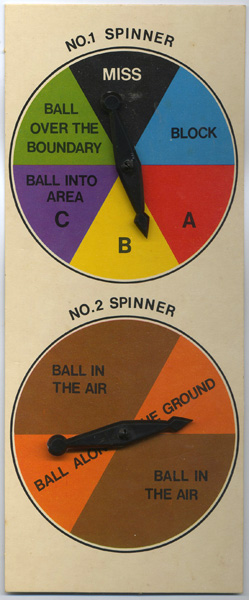
\includegraphics[height=2in]{img/family-cricket-spinner.jpg}
\end{minipage}
\vfill
\hfill {\tiny Image source: \url{http://replaycricket.com/2010/10/29/family-cricket/}}

\sld{Repeated i.i.d. Binary Trials}
\begin{itemize}
\item Suppose the outcome is binary and assigned to 0 or 1; e.g., 
\begin{subitemize}
\item 20\% chance of outcome 1: \emph{ball in play}
\item 80\% chance of outcome 0: \emph{ball \emph{not} in play}
\end{subitemize}
\item Consider different numbers of bowls delivered.
\item How will proportion of successes in sample differ?
\end{itemize}

\sld{Simulating i.i.d. Binary Trials}
\begin{itemize}
\item R Code: {\small \code{rbinom(10, N, 0.2) / N}}
\begin{subitemize}
\item {\bfseries 10 bowls} \hfill (10\% to 50\% success rate)
\\[4pt] 2 3 5 2 4 1 2 2 1 1
\vspace*{3pt}
%
\item {\bfseries 100 bowls} \hfill (16\% to 26\% success rate)
\\[4pt] 26 18 23 17 21 16 21 15 21 26
\vspace*{3pt}
%
\item {\bfseries 1000 bowls} \hfill (18\% to 22\% success rate)
\\[4pt] 181 212 175 213 216 179 223 198 188 194
\vspace*{3pt}
%
\item {\bfseries 10,000 bowls} \hfill (19.3\% to 20.3\% success rate)
\\[4pt] 2029 1955 1981 1980 2001 2014 1931 1982 1989 2020
\end{subitemize}
\end{itemize}

\sld{Simple Point Estimation}
%
\begin{itemize}
\item Estimate chance of success $\theta$ by proportion of successes:
\[
\theta^{*} = \frac{\text{successes}}{\text{attempts}}
\]
\item Simulation shows accuracy depends on the amount of data.
\item Statistics is about quantifying uncertainty.
\item Bayesian statistics is about using uncertainty in inference.
\end{itemize}

\sld{Confidence via Simulation}
%
\begin{itemize}
\item Estimator uncertainty (\emph{not} Bayesian posterior)
{\small
\begin{Verbatim}
num_sims <- 10000
N <- 100;  
theta <- 0.2;
hist(rbinom(num_sims, N, theta) / N,
     main=sprintf("%d simulations",N), xlab="theta*");
\end{Verbatim}
}
\vspace*{-12pt}
\begin{center}
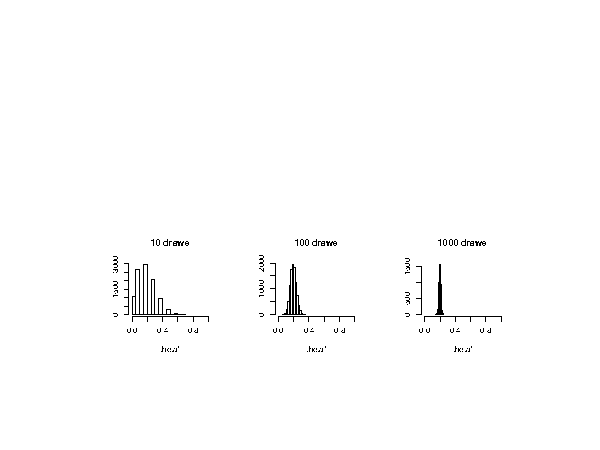
\includegraphics[width=0.8\textwidth]{img/hist-10-100-1000.pdf}
\end{center}

\end{itemize}

\sld{Example Interval Calculation}
\begin{itemize}
\item \emph{$P\%$ confidence interval:}  interval in which $P\%$ of the estimates are
expected to fall.
\item Simulation computes intervals to any accuracy.
\item Simulate, sort, and inspect the central empirical interval.
{\small
\begin{Verbatim}
> sims <- rbinom(10000, 1000, 0.2) / 1000
> sorted_sims <- sort(sims)
> sorted_sims[c(250, 9750)]
[1] 0.176 0.225
\end{Verbatim}
}
\item The 95\% confidence interval is thus $(0.176,0.225)$
\item i.e., if true $\theta = 0.2$, then 95\% of the samples of
  size 1000 used will produce estimates in $(0.176,0.225)$
\end{itemize}


\sld{Estimator Bias}
\begin{itemize}
\item {\bfseries Bias:} expected difference of estimate from true value
\item Continuing previous example
{\small
\begin{Verbatim}
> sims <- rbinom(10000, 1000, 0.2) / 1000
> mean(sims)
[1] 0.2002536
\end{Verbatim}
}
\item Value of 0.2 is estimate of expectation
\item Shows this estimator is \emph{unbiased}
\end{itemize}

\sld{Simple Point Estimation (cont.)}
\begin{itemize}
\item {\bfseries Central Limit Theorem:}  \emph{expected} error in $\theta^*$ goes down as
{\Large
\[
\frac{1}{\sqrt{N}}
\]
}
\item Each decimal place of accuracy requires $100 \times$ more samples.
\item Width of confidence intervals shrinks at the same rate.
\vfill
\item Can also use theory to show this estimator is unbiased.
\end{itemize}

\sld{Pop Quiz! Cancer Clusters}
%
\begin{itemize}
\item Why do lowest and highest cancer clusters look so similar?
\end{itemize}
\vspace*{1pt}
\begin{center}
\hfill
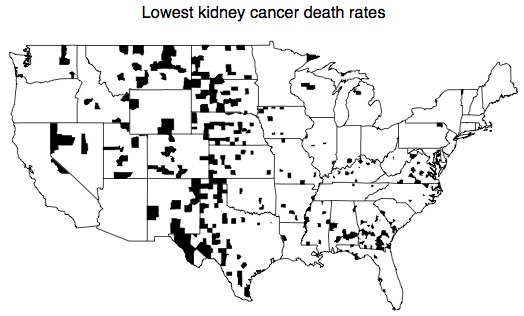
\includegraphics[width=0.45\textwidth]{img/low-cancer.jpg}
\hfill
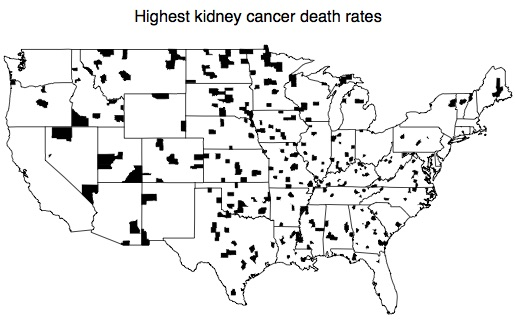
\includegraphics[width=0.45\textwidth]{img/high-cancer.jpg}
\hfill
\end{center}
\vfill
\hfill {\tiny Image from Gelman et al., {\slshape Bayesian Data Analysis, 3rd Edition} (2013)}

\sld{Pop Quiz Answer}
%
\begin{itemize}
\item Hint: mix earlier simulations of repeated i.i.d. trials with 20\% success and sort:
{\footnotesize
\begin{center}
\begin{tabular}{ccccc}
1/10 &  1/10 &  1/10 &  15/100 &  16/100
\\
17/100 &  175/1000 &  179/1000 &  18/100 &  181/1000
\\
188/1000 &  194/1000 &  198/1000 & 2/10 &  2/10 
\\
2/10 &  2/10 & 21/100 &  21/100 &  21/100 
\\
212/1000 &  213/1000 &   216/1000 &   223/1000 &  23/100
\\
26/100 &  26/100 &  3/10 &  4/10 &  5/10 
\end{tabular}
\end{center}
}
\item More variation in observed rates with smaller sample sizes
\vfill
\item \emph{Answer}: High cancer and low cancer counties are small populations
\end{itemize}




\mypart{Warmup Exercise II}{Maximum Likelihood \\[8pt]\spc Estimation}

\sld{Observations, Counterfactuals,
     \\[6pt] \spc{}and Random Variables}
\begin{itemize}
\item Assume we observe data $y = y_1, \ldots, y_N$
\item Statistical modeling assumes even though $y$ is observed,
the values could have been different
\item John Stuart Mill first characterized this {\bfseries counterfactual} nature of statistical modeling in:
\\[3pt] {\slshape A System of Logic, Ratiocinative and Inductive} (1843)
\item In measure-theoretic language, $y$ is a {\bfseries random variable}
\end{itemize}

\sld{Likelihood Functions}
%
\begin{itemize}
\item A \myemph{likelihood function} is a probability function (density, mass, or mixed) 
\[
p(y|\theta,x),
\]
where
\begin{subitemize}
\item $\theta$ is a vector of \myemph{parameters}, 
\item $x$ is some fixed \myemph{unmodeled data} (e.g., regression predictors or
  ``features''),
\item $y$ is some fixed \myemph{modeled data} (e.g., observations)
\end{subitemize}
\item considered as a function $\mathcal{L}(\theta)$ of $\theta$ for fixed $x$ and $y$.
\end{itemize}

\sld{Maximum Likelihood Estimation}
\begin{itemize}
\item \myemph{Estimate} parameters $\theta$ given observations $y$.
\item Maximum likelihood estimation (MLE) chooses 
estimate that maximizes the likelihood function, i.e.,
\[
\theta^* 
\ = \ \argmax_{\theta} \ \mathcal{L}(\theta) 
\ = \ \argmax_{\theta} \ p(y|\theta,x)
\]
\item This function of $\mathcal{L}$ and $y$ (and $x$) is called an \myemph{estimator}
\end{itemize}

\sld{Example of MLE}
%
\begin{itemize}
\item The frequency-based estimate 
\[
\theta^{*} = \frac{1}{N} \sum_{n=1}^N y_n, 
\]
is the observed rate of ``success'' (outcome 1) observations.
\item This is the MLE for the model
\[
p(y|\theta) 
\ = \ \prod_{n=1}^N p(y_n|\theta) 
\ = \  \prod_{n=1}^N \distro{Bernoulli}(y_n|\theta) 
\]
where for $u \in \setcomp{0,1}$, 
{\small
\[
\distro{Bernoulli}(u|\theta) = 
\begin{cases}
\theta & \text{if } u = 1 
\\
1 - \theta & \text{if } u = 0
\end{cases}
\]
}
\end{itemize}

\sld{Example of MLE {\normalsize (cont.)}}
\vspace*{-4pt}
\begin{itemize}
\item First modeling \emph{assumption} is that data are i.i.d.,
\[
p(y|\theta) = \prod_{n=1}^N p(y_n|\theta)
\] 
\item Second modeling \emph{assumption} is form of likelihood,
\[
p(y_n|\theta) = \distro{Bernoulli}(y_n|\theta)
\]
\end{itemize}

\sld{Example of MLE {\normalsize (cont.)}}
\begin{itemize}
\item The frequency-based estimate is the MLE
\item First derivative is zero (indicating min or max),
\[
\mathcal{L}'_y(\theta^*) = 0,
\]
\item Second derivative is negative (indicating max),
\[
\mathcal{L}''_y(\theta^*) < 0.
\]
\end{itemize}

\sld{MLEs can be Dangerous!}
\begin{itemize}
\item Recall the cancer cluster example
\item Accuracy is low with small counts
\item What we need are hierarchical models (stay tuned)
\end{itemize}

\mypart{Part I}{Bayesian Inference}

\sld{Bayesian Data Analysis}
\begin{itemize}
\item ``By {Bayesian data analysis}, we mean {practical methods}
  for making {inferences} from {data} using {probability models}
  for quantities we {observe} and about which we {wish to learn}.''
  % 
\item ``The essential characteristic of Bayesian methods is
  their \myemph{explict use of probability for quantifying uncertainty}
  in inferences based on statistical analysis.''
\end{itemize}
% 
\vfill\hfill{\footnotesize Gelman et al., {\slshape Bayesian Data Analysis},
  3rd edition, 2013}

\sld{Bayesian Methodology}
% 
\begin{itemize}
\item Set up \myemph{full probability model}
  \vspace*{-4pt}
  \begin{itemize}
  \item for all observable \& unobservable quantities
  \item consistent w. problem knowledge \& data collection
  \end{itemize}
  % 
\item \myemph{Condition} on observed data
  \vspace*{-4pt}
  \begin{itemize}
  \item to caclulate posterior probability of unobserved quantities
    (e.g., parameters, predictions, missing data)
  \end{itemize}
  % 
\item \myemph{Evaluate}
  \vspace*{-4pt}
  \begin{itemize}
  \item model fit and implications of posterior
  \end{itemize}
\vfill
\item \myemph{Repeat} as necessary
\end{itemize}

\vfill\hfill {\footnotesize {\slshape Ibid.}}

\sld{Where do Models Come from?}
\begin{itemize}
\item Sometimes model comes first, based on substantive
  considerations
\begin{subitemize}
\item toxicology, economics, ecology, \ldots
\end{subitemize}
\item Sometimes model chosen based on data collection
\begin{subitemize}
\item  traditional statistics of surveys and experiments
\end{subitemize}
\item Other times the data comes first
\begin{subitemize}
\item observational studies, meta-analysis, \ldots
\end{subitemize}
\hfill
\item Usually its a mix
\end{itemize}

\sld{(Donald) Rubin's Philosophy}
\begin{itemize}
\item All statistics is inference about missing data
\item Question 1: What would you do if you had all the data?
\item Question 2: What were you doing before you had any data?
\vfill
\hfill {\footnotesize (as relayed in course notes by Andrew Gelman)}
\end{itemize}

\sld{Model Checking and Improvement}
\begin{itemize}
\item Do the inferences make sense?
\item Are the model's predictions consistent with the data? 
\item {\slshape \myemph{Not}}: Is the model true?
\item {\slshape \myemph{Not}}: What is Pr[model is true]?
\item {\slshape \myemph{Not}}: Can we ``reject'' the model?
\vfill
\item Expanding the model
\item Including more data
\end{itemize}

\sld{Model Checking (cont.)}
\begin{itemize}
\item Check parameter inferences
\begin{subitemize}
\item Do they make sense?
\item Are they consistent with model's prior specification?
\end{subitemize}
\item Check fit to data
\item Check predictions on new data
\end{itemize}


\sld{Using Bayesian Inference}
\begin{itemize}
\item Finds parameters consistent with prior info and
  data$^*$
\begin{subitemize}
\item $^*$ if such agreement is possible
\end{subitemize}
\item Automatically includes uncertainty and variability
\item Inferences can be plugged in directly
\begin{subitemize}
\item risk assesment
\item decision analysis
\end{subitemize}
\end{itemize}

\sld{Notation for Basic Quantities}
% 
\begin{itemize}
\item \myemph{Basic Quantities}
\begin{subitemize}
\item $y$: \ observed data
\item $\theta$: \ parameters (and other unobserved quantities)
\item $x$: \ constants, predictors for conditional (aka ``discriminative'') models
\end{subitemize}
\item \myemph{Basic Predictive Quantities}
\begin{subitemize}
\item $\tilde{y}$: unknown, potentially observable quantities
\item $\tilde{x}$: \ constants, predictors for unknown quantities
\end{subitemize}
\end{itemize}

\sld{Naming Conventions}

\begin{itemize}
\item \myemph{Joint}: \ $p(y,\theta)$
\item \myemph{Sampling / Likelihood}: \ $p(y|\theta)$
\begin{subitemize}
\item Sampling is function of $y$ with $\theta$ fixed (prob function)
\item Likelihood is function of $\theta$ with $y$ fixed (\emph{not} prob function)
\end{subitemize}
\item \myemph{Prior}: \ $p(\theta)$
\item \myemph{Posterior}: \ $p(\theta|y)$
\item \myemph{Data Marginal (Evidence)}: \ $p(y)$
\item \myemph{Posterior Predictive}: \ $p(\tilde{y}|y)$
\end{itemize}


\sld{Bayes's Rule for Posterior}
% 
\vspace*{-4pt}
\begin{eqnarray*}
    p(\theta|y) 
    & = & \frac{p(y,\theta)}{p(y)} 
          \hspace*{64pt} \text{\small [def of conditional]}
    \\[6pt]
    & = & \frac{p(y|\theta) \, p(\theta)}{p(y)}
          \hspace*{44pt} \text{\small [chain rule]}
    \\[6pt]
    & = & \frac{p(y|\theta) \, p(\theta)}{\int_{\Theta} p(y,\theta') \ d\theta'}
          \hspace*{40pt} \text{\small [law of total prob]}
    \\[6pt]
    & = & \frac{p(y|\theta) \, p(\theta)}{\int_{\Theta} p(y|\theta') \,
      p(\theta') \ d\theta'}
          \hspace*{20pt} \text{\small [chain rule]}
\end{eqnarray*}
\vfill
\begin{itemize}
\item \emph{Inversion:} Final result depends only on 
  sampling distribution (likelihood) $p(y|\theta)$ and prior
  $p(\theta)$
\end{itemize}

\sld{Bayes's Rule up to Proportion}
\begin{itemize}
\item If data $y$ is fixed, then
\begin{eqnarray*}
p(\theta|y) 
& = & \frac{p(y|\theta) \, p(\theta)}{p(y)}
\\[6pt]
& \propto & p(y|\theta) \, p(\theta) 
\\[6pt]
& = & p(y,\theta)
\end{eqnarray*}
\item Posterior proportional to likelihood times prior
\item Equivalently, posterior proportional to joint
\end{itemize}

\sld{Posterior Predictive Distribution}
\begin{itemize}
\item Predict new data $\tilde{y}$ based on observed data $y$
\item Marginalize out parameters from posterior
\[
p(\tilde{y}|y)
\ = \
\int_{\Theta} p(\tilde{y}|\theta) \, p(\theta | y) \, d\theta.
\]
\item Averages predictions $p(\tilde{y}|\theta)$,
weight by posterior $p(\theta|y)$
\begin{subitemize}
\item $\Theta = \setcomp{\theta \ | \ p(\theta|y) > 0}$ is support
  of $p(\theta|y)$
\end{subitemize}
\item Allows continuous, discrete, or mixed parameters
\begin{subitemize}
\item integral notation shorthand for sums and/or integrals
\end{subitemize}
\end{itemize}

\sld{Event Probabilities}
\begin{itemize}
\item Recall that an event $A$ is a collection of outcomes
\item Suppose event $A$ is determined by indicator on parameters
\[
f(\theta) 
= 
\begin{cases}
1 & \text{if } \theta \in A
\\
0 & \text{if } \theta \not\in A
\end{cases}
\]
\item e.g., $f(\theta) = \theta_1 > \theta_2$ 
\ \ for \ \ $\Prob{\theta_1 > \theta_2 \, | \, y}$
\item Bayesian event probabilities calculate posterior mass
\[
\Prob{A} = \int_{\Theta} f(\theta) \, p(\theta|y) \, d\theta.
\]
\item Not frequentist, because involves parameter probabilities
\end{itemize}

\mypart{Example I}{Male Birth Ratio}

\sld{Laplace's Data and Problems}
\begin{itemize}
\item Laplace's data on live births in Paris from 1745--1770: 
\begin{center}\small
\begin{tabular}{c|c}
{\slshape sex} & {\slshape live births}
\\ \hline
female & 241\,945 
\\
male & 251\,527
\end{tabular}
\end{center}
\item Question 1 (Event Probability) 
\\  
Is a boy more likely to be born than a girl?
\item Question 2 (Estimate) 
\\  
What is the birth rate of boys vs. girls?
\item Bayes formulated the basic binomial model
\item Laplace solved the integral
\end{itemize}

\sld{Binomial Distribution}
\begin{itemize}
\item Binomial distribution is number of successes $y$ in $N$ 
i.i.d. Bernoulli trials with chance of success $\theta$
\item If $y_1,\ldots,y_N\sim \distro{Bernoulli}(\theta)$, 
\\[4pt] then $(y_1 + \cdots + y_N) \sim \distro{Binomial}(N,\theta)$
\item The analytic form is
\[
\distro{Binomial}(y|N,\theta) 
\ = \ \binom{N}{y} \theta^{y} (1 - \theta)^{N-y}
\]
where the binomial coefficient normalizes for permutations (i.e.,
which subset of $n$ has $y_n = 1$),
\[
\binom{N}{y} = \frac{N!}{y! \, (N-y)!}
\]
\end{itemize}

\sld{Bayes's Binomial Model}
\begin{itemize}
\item{Data}
\begin{subitemize}
\item $y$: total number of male live births (241,945)
\item $N$ : total number of live births (493,472)
\end{subitemize}
\item Parameter
\begin{subitemize}
\item $\theta \in (0,1)$: proportion of male live births
\end{subitemize}
\item Likelihood
\[
p(y|N,\theta) 
\ = \ \distro{Binomial}(y|N,\theta) 
\ = \ \binom{N}{y} \theta^{y} (1 - \theta)^{N-y}
\]
\item Prior
\[
p(\theta) 
\ = \ \distro{Uniform}(\theta \, | \, 0,1) 
\ = \ 1
\]
\end{itemize}

\sld{Beta Distribution}
\begin{itemize}
\item Required for analytic posterior of Bayes's model
\item For parameters $\alpha,\beta > 0$ and $\theta \in (0,1)$,
\[
\distro{Beta}(\theta|\alpha,\beta) 
\ = \ \frac{1}{\Betafun(\alpha,\beta)} 
      \theta^{\alpha - 1} \, 
      (1 - \theta)^{\beta-1}
\] 
\item Euler's Beta function is used to normalize,
\[
\Betafun(\alpha,\beta) 
\ = \ \int_0^1 u^{\alpha-1}(1-u)^{\beta-1} du
\ = \ \frac{\Gamma(\alpha)\,\Gamma(\beta)}{\Gamma(\alpha + \beta)}
\]
where $\Gamma()$ is continuous generalization of factorial
\item Note: \ $\distro{Beta}(\theta|1,1) = \distro{Uniform}(\theta|0,1)$
\end{itemize}

\sld{Beta Distribution --- Examples}
\vspace*{-4pt}
\begin{itemize}
\item Unnormalized posterior density assuming uniform prior and $y$
  successes out of $n$ trials (all with mean 0.6).
\end{itemize}
\begin{center}
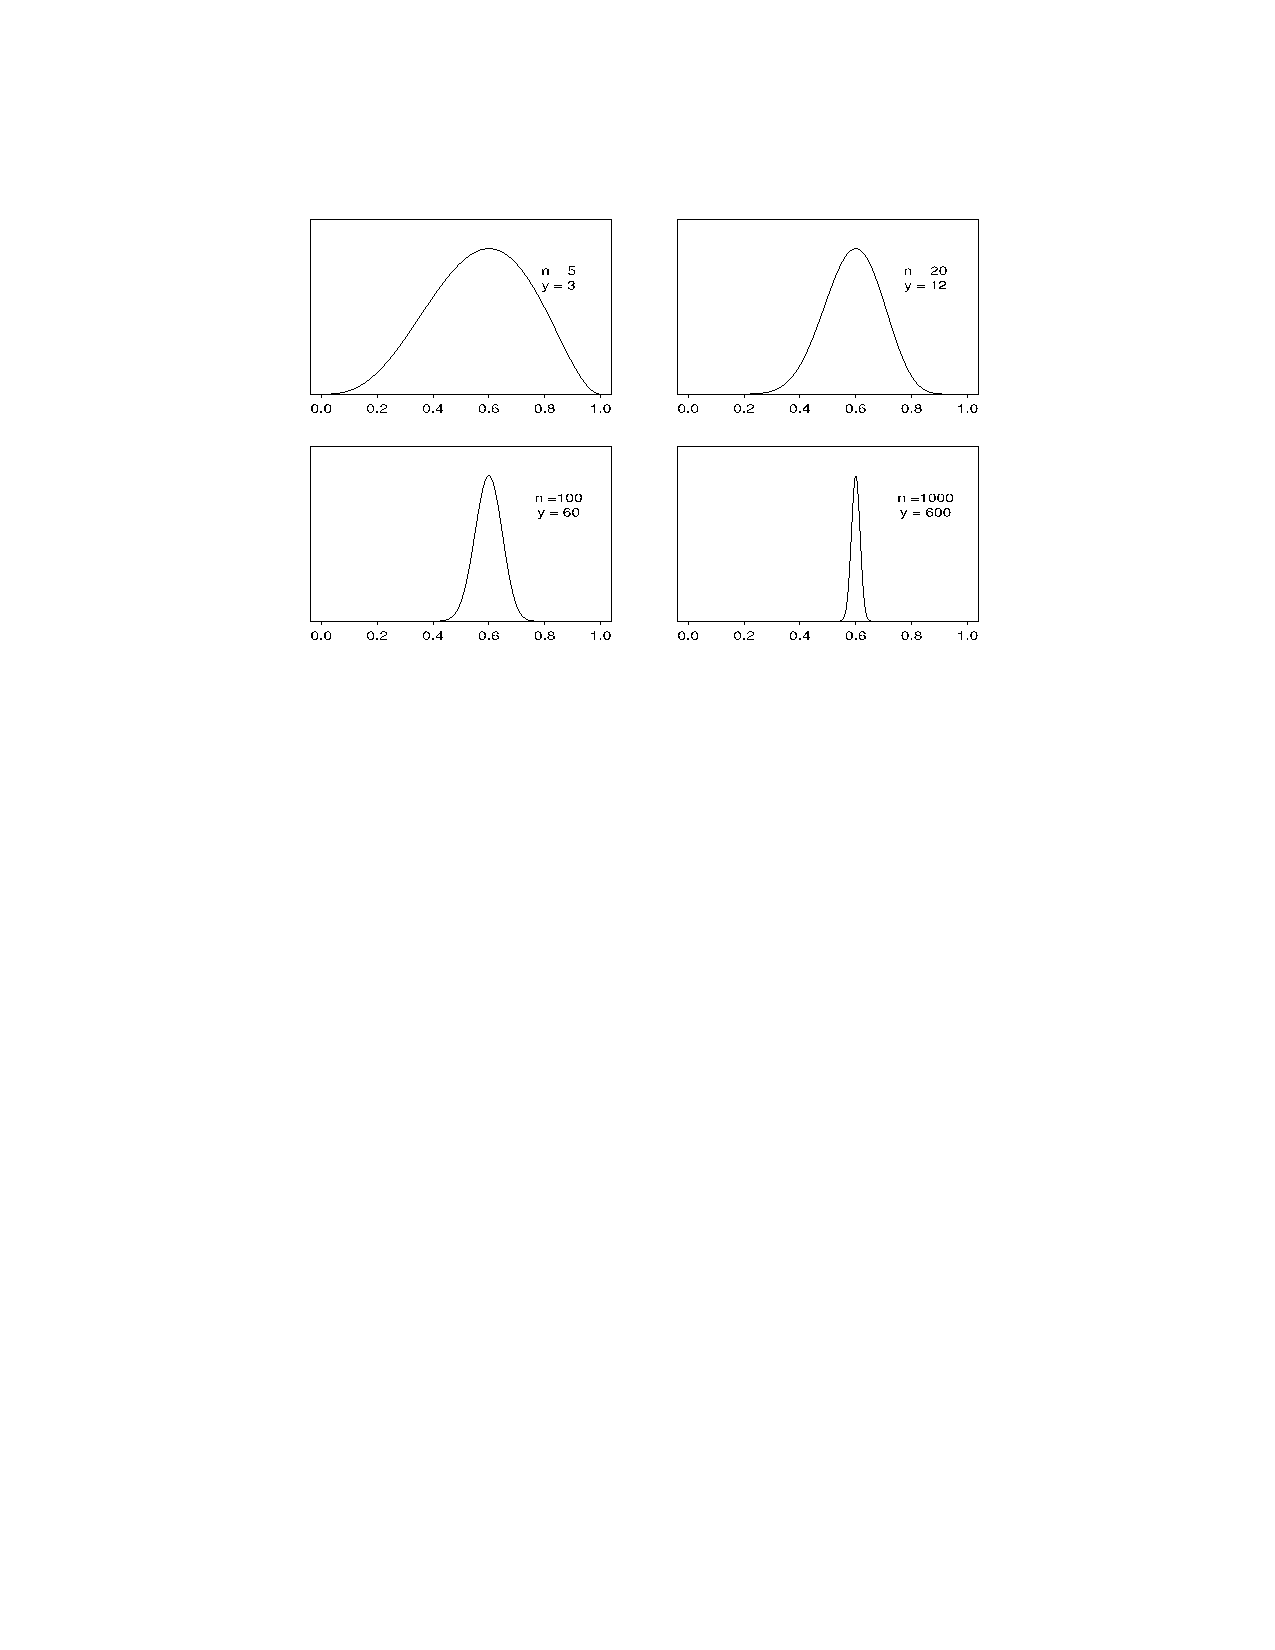
\includegraphics[height=1.6in]{img/bda-beta-plots.pdf}
\end{center}
\vspace*{-12pt}
\hfill {\tiny Gelman et al. (2013) {\slshape Bayesian Data Analysis},
  3rd Edition.}

\sld{Laplace Turns the Crank}
\begin{itemize}
\item Given Bayes's general formula for the posterior
\[
p(\theta|y,N) 
\ = \ 
\frac{\distro{Binomial}(y|N,\theta) \, \distro{Uniform}(\theta|0,1)}
     {\int_{\Theta} \distro{Binomial}(y|N,\theta') \,  p(\theta')
       d\theta'}
\]
\item Laplace used Euler's Beta function (B) to normalize the
  posterior, with final solution
\[
p(\theta|y,N) 
\ = \ \distro{Beta}(\theta \, | \, y + 1, \ N - y + 1)
\]
\end{itemize}

\sld{Estimation}
\begin{itemize}
\item Posterior is $\distro{Beta}(\theta \, | \, 1 + 241\,945, \ 1 + 251\,527)$
\item Posterior mean: 
\[
\frac{1 + 241\,945}
     {1 + 241\,945 + 1 + 251\,527}
\approx 0.490291{\bf3}
\]
\item Maximum likelihood estimate same as posterior mode (because
  of uniform prior) 
\[
\frac{241\,945}
     {241\,945 + 251\,527}
\approx 0.490291{\bf2}
\]
\item As number of observations approaches $\infty$, 
\\
MLE approaches posterior mean
\end{itemize}

\sld{Event Probability Inference}
\begin{itemize}
\item What is probability that a male live birth is more likely than a
  female live birth?
\begin{eqnarray*}
\Prob{\theta > 0.5} 
& = &  \int_{\Theta} \indicator{\theta > 0.5} \, p(\theta|y,N) d\theta
\\[4pt]
& = &  \int_{0.5}^1 p(\theta|y,N) d\theta
\\[4pt]
& = &  1 - F_{\theta|y,N}(0.5)
\\[4pt]
& \approx &  10^{-42}
\end{eqnarray*}
\item $\indicator{\phi} = 1$ if condition $\phi$ is true and 0 otherwise.
\item  $F_{\theta|y,N}$ is posterior cumulative distribution
function (cdf).
\end{itemize}

\sld{Bayesian ``Fisher Exact Test''}
\vspace*{-4pt}
\begin{itemize}
\item Suppose we observe the following data on handedness
\begin{center}
{\small
\begin{tabular}{c|c|c||c}
     & {\slshape sinister} & {\slshape dexter} & TOTAL
\\ \hline \hline
{\slshape male} & 9 ($y_1$) & 43 & 52 ($N_1$)
\\
{\slshape female} & 4 ($y_2$) & 44 & 48 ($N_2$)
\end{tabular}
}
\end{center}
\item Assume likelihoods $\distro{Binomial}(y_k|N_k,\theta_k)$, uniform
  priors
\item Are men more likely to be lefthanded?
{\small
\begin{eqnarray*}
\Prob{\theta_1 > \theta_2 \, | \, y, N}
& = & 
\int_{\Theta} \indicator{\theta_1 > \theta_2} \, p(\theta|y,N) \, d\theta
\\[8pt]
& \approx &  0.91
\end{eqnarray*}
\item Directly interpretable result; \emph{not} a frequentist procedure
}
\end{itemize}


\sld{Visualizing Posterior Difference}
\begin{itemize}
\item Plot of posterior difference, $p(\theta_1 - \theta_2 \, | \, y,
  N)$ (men - women)
\begin{center}
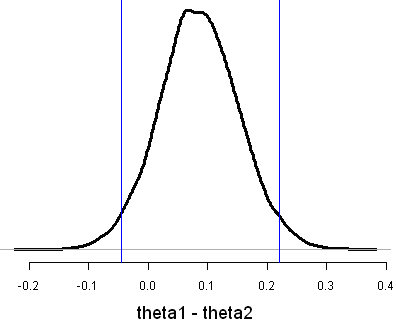
\includegraphics[height=1.5in]{img/bayesian-exact-posterior-handedness.png}
\end{center}
\item Vertical bars: central 95\% posterior interval $(-0.05,0.22)$
\end{itemize}


\mypart{Part III}{Conjugate Priors}

\sld{Conjugate Priors}
\begin{itemize}
\item Family $\mathcal{F}$ is a conjugate prior for family
  $\mathcal{G}$ if
\begin{subitemize}
\item prior in $\mathcal{F}$ and
\item likelihood in $\mathcal{G}$,
\item entails posterior in $\mathcal{F}$
\end{subitemize}
\item Before MCMC techniques became practical, Bayesian analysis
  mostly involved conjugate priors
\item Still widely used because analytic solutions are more efficient
  than MCMC
\end{itemize}

\sld{Beta is Conjugate to Binomial}
\vspace*{-2pt}
\begin{itemize}
\item Prior: \ \ \ \ \ \ \ \ \ \ \ $p(\theta|\alpha,\beta) =
  \distro{Beta}(\theta|\alpha,\beta)$
\item Likelihood: \ \ $p(y|N,\theta) = \distro{Binomial}(y|N,\theta)$
\item Posterior:
{\small
\begin{eqnarray*}
p(\theta|y,N,\alpha,\beta)
& \propto & p(\theta|\alpha,\beta) \, p(y|N,\theta)
\\[6pt]
& = & \distro{Beta}(\theta|\alpha,\beta) 
      \, \distro{Binomial}(y|N,\theta)
\\
& = & \frac{1}{\Betafun(\alpha,\beta)} 
      \theta^{\alpha - 1} \, 
      (1 - \theta)^{\beta-1}
      \ \
      \binom{N}{y} \theta^{y} (1 - \theta)^{N-y}
\\[6pt]
& \propto & 
      \theta^{y + \alpha - 1} \, 
      (1 - \theta)^{N - y + \beta - 1}
\\[6pt]
& \propto & \distro{Beta}(\theta|\alpha + y, \ \beta + (N - y))
\end{eqnarray*}
}
\end{itemize}

\sld{Chaining Updates}
\vspace*{-4pt}
\begin{itemize}
\item Start with prior $\distro{Beta}(\theta|\alpha,\beta)$
\item Receive binomial data in $K$ statges $(y_1, N_1), \ldots, (y_K, N_K)$
\item After $(y_1,N_1)$, posterior is 
  $\distro{Beta}(\theta|\alpha + y_1, \ \beta + N_1 - y_1)$
\item Use as prior for $(y_2,N_2)$, with posterior \\[3pt]
  $\distro{Beta}(\theta|\alpha + y_1 + y_2, \ \ \beta + (N_1 -
  y_1) + (N_2 - y_2))$
\item Lather, rinse, repeat, until final posterior
\[
\distro{Beta}(\theta|\alpha + y_1 + \cdots + y_K, \ \ \beta + (N_1 +
\cdots + N_K) - (y_1 + \cdots + y_K))
\]
\item Same result as if we'd updated with combined data \\[3pt]
$\distro{Beta}(y_1 + \cdots + y_K, \ \ N_1 + \cdots + N_K)$
\end{itemize}


\mypart{Part II}{(Un-)Bayesian \\[8pt]\spc{}Point Estimation}

\sld{MAP Estimator}
\vspace*{-4pt}
\begin{itemize}
\item For a Bayesian model $p(y,\theta) = p(y|\theta) \, p(\theta)$,
the max a posteriori (MAP) estimate maximizes the posterior,
\begin{eqnarray*}
\theta^{*} 
& = & \argmax_{\theta} \ p(\theta|y)
\\[3pt]
& = & \argmax_{\theta} \ \frac{\displaystyle p(y|\theta) p(\theta)}{p(y)}
\\[3pt]
& = & \argmax_{\theta} \ p(y|\theta) p(\theta).
\\[3pt]
& = & \argmax_{\theta} \ \log p(y|\theta) + \log p(\theta).
\end{eqnarray*}
\item \emph{not} Bayesian because it doesn't integrate over uncertainty
\item \emph{not} frequentist because of distributions over parameters

\end{itemize}

\sld{MAP and the MLE}
\begin{itemize}
\item MAP estimate reduces to the MLE if the prior is uniform, i.e.,
\[
p(\theta) = c
\]
because
\begin{eqnarray*}
\theta^{*} & = & \argmax_{\theta} \ p(y|\theta) \, p(\theta)
\\[4pt]
& = & \argmax_{\theta} \ p(y|\theta) \, c
\\[4pt]
& = & \argmax_{\theta} \ p(y|\theta).
\end{eqnarray*}
\end{itemize}

\sld{Penalized Maximum Likelihood}
\begin{itemize}
\item The MAP estimate can be made palatable to frequentists 
via philosophical sleight of hand 
\item Treat the negative log prior $-\log p(\theta)$ as a ``penalty''
\item e.g., a $\distro{Normal}(\theta|\mu,\sigma)$ prior becomes a penalty function 
\[
\lambda_{\theta, \mu,\sigma}
\  = \ 
-\left( 
   \log \sigma + \frac{1}{2}\left(\frac{\theta -  \mu}{\sigma}\right)^2 
 \right)
\]
\item Maximize sum of log likelihood and negative penalty
\begin{eqnarray*}
\theta^{*} 
& = & \argmax_{\theta} \ \log p(y|\theta,x) - \lambda_{\theta,\mu,\sigma}
\\[4pt]
& = & \argmax_{\theta} \ \log p(y|\theta,x) + \log p(\theta|\mu,\sigma)
\end{eqnarray*}
\end{itemize}

\sld{Proper Bayesian Point Estimates}
\begin{itemize}
\item Choose estimate to minimize some loss function
\item To minimize expected squared error (i.e., L2 loss), use
$\expectation{(\theta - \theta')^2 \, | \, y}$, use the posterior mean
\[
\hat{\theta}
\ = \ \argmin_{\theta'} \expectation{(\theta - \theta')^2 \, | \, y}
\ = \ \int_{\Theta} \theta \times p(\theta|y) \, d\theta.
\]
\item To minimize expected absolute error (L1 loss), $\expectation{|\theta -
    \theta'|}$, use the posterior median.
\item Other loss (utility) functions possible, the study of which falls under
  decision theory
\item All share property of involving full Bayesian inference.
\end{itemize}


\sld{Point Estimates for Inference?}
\begin{itemize}
\item Common in machine learning to generate a point estimate
  $\theta^*$, then use it for inference, $p(\tilde{y} | \theta^{*})$
\item This is \emph{defective} because it
\vspace*{-1pt}
\begin{center}
{\Large\bfseries Underestimates Uncertainty}
\end{center}
\item To properly estimate uncertainty, apply full Bayes
\item If not, (probabilistic) Dutch book can be made against you
\begin{subitemize}
\item i.e., if you use your strategy to bet, I can beat you 
in the long run using full Bayes (de Finetti)
\end{subitemize}
\end{itemize}

\mypart{Part III}{Philosophical Interlude}

\sld{Exchangeability}
\begin{itemize}
\item Roughly, an exchangeable probability function is such that for
a sequence of random variables $y = y_1,\ldots,y_N$,
\[
p(y) = p(\pi(y))
\]
for every $N$-permutation $\pi$ (i.e, a one-to-one mapping of $\setcomp{1,\ldots,N}$)
\item i.i.d. implies exchangeability, but not vice-versa
\end{itemize}

\sld{Exchangeability Assumptions}
%
\begin{itemize}
\item Models almost always make some kind of exchangeability assumption
\item Typically when other knowledge is not available
\begin{subitemize}
\item e.g., treat voters as conditionally i.i.d. given their age, 
sex, income, education level, religous affiliation, 
and state of residence
\item But voters have many more properties (hair color, height, profession, employment status, marital status, car ownership, gun ownership, etc.)
\item Missing predictors introduce additional error (on top of measurement error)
\end{subitemize}
\end{itemize}


\sld{de Finetti's Theorem}
\begin{itemize}
\item Given some background variables, every exchangeable sequence is conditionally i.i.d.
\item So if our i.i.d. assumptions are invalid, 
\\ condition on more predictors
\end{itemize}

\sld{Bayesian vs.\ Frequentist}
\begin{itemize}
\item \emph{Everyone}: Model data $y$ as ``random''
\item \emph{Everyone}: Parameters have single, true (but unknown) value
\item \emph{Everyone}: Admit Bayes's rule of probability
\item \emph{Bayesians Only}: Model parameters $\theta$ as ``random''
\item \emph{Frequentists Only}: Probabilities are long-run frequencies of observables, which excludes parameters (unobservable)
\item \emph{Bayesians Only}: Allow probabilities conditioned on parameters
\end{itemize}

\sld{Random Parameters:\\[8pt]\spc{}\!Doxastic or Epistemic?}
\begin{itemize}
\item Bayesians treat distributions over parameters as epistemic \\
(i.e., about knowledge) 
\item They do \emph{not} \ treat them as being doxastic \\
(i.e., about beliefs)
\item Priors encode our knowledge before seeing the data
\item Posteriors encode our knowledge after seeing the data
\item Bayes's rule provides the way to update our knowledge
\item People like to pretend models are ontological \\
(i.e., about what exists)
\end{itemize}

\sld{Arbitrariness:\\[8pt]\spc{}\!Priors vs.\ Likelihood}
\begin{itemize}
\item Bayesian analyses often criticized as subjective (arbitrary)
\item Choosing priors is no more arbitrary than choosing a likelihood
  function (or an exchangeability/i.i.d.\ assumption)
\item As George Box famously wrote (1987),
\begin{center}
\large
{\bfseries All models are wrong, but some are useful.}
\end{center}
\item This is true for frequentists as well as Bayesians
\end{itemize}


\mypart{Part IV}{Hierarchical Models}

\sld{Baseball At-Bats}
\begin{itemize}
\item For example, consider baseball batting ability.
\begin{subitemize}
\item 
{\footnotesize Baseball is sort of like cricket, but with round bats, a
  one-way field, stationary ``bowlers'', four bases, short games, 
  and no draws}
\end{subitemize}
\item Batters have a number of ``at-bats'' in a season, out of which they
  get a number of ``hits'' (hits are a good thing)
\item Nobody with higher than 40\% success rate since 1950s.
\item No player (excluding ``bowlers'') bats much less than 20\%.
\item Same approach applies to hospital pediatric surgery
  complications (a BUGS example), reviews on Yelp,
  test scores in multiple classrooms, \ldots
\end{itemize}


\sld{Baseball Data}
\\
%
\begin{minipage}[t]{0.49\textwidth}
\begin{itemize}
\item Hits versus at bats for the 2006 American League season
\item Not much variation in ability!
\item Ignore skill vs. at-bats relation
\item Note uncertainty of MLE
\end{itemize}
\end{minipage}
%
\begin{minipage}[t]{0.50\textwidth}
\begin{center}
\vspace*{-36pt}
\hfill 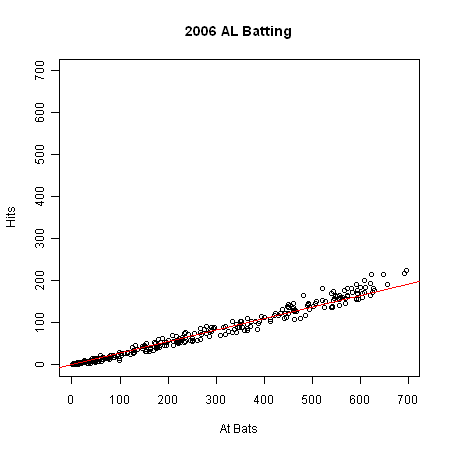
\includegraphics[height=1.4in]{img/al06hitsvsatbats.png}
\\[-18pt]
\hfill 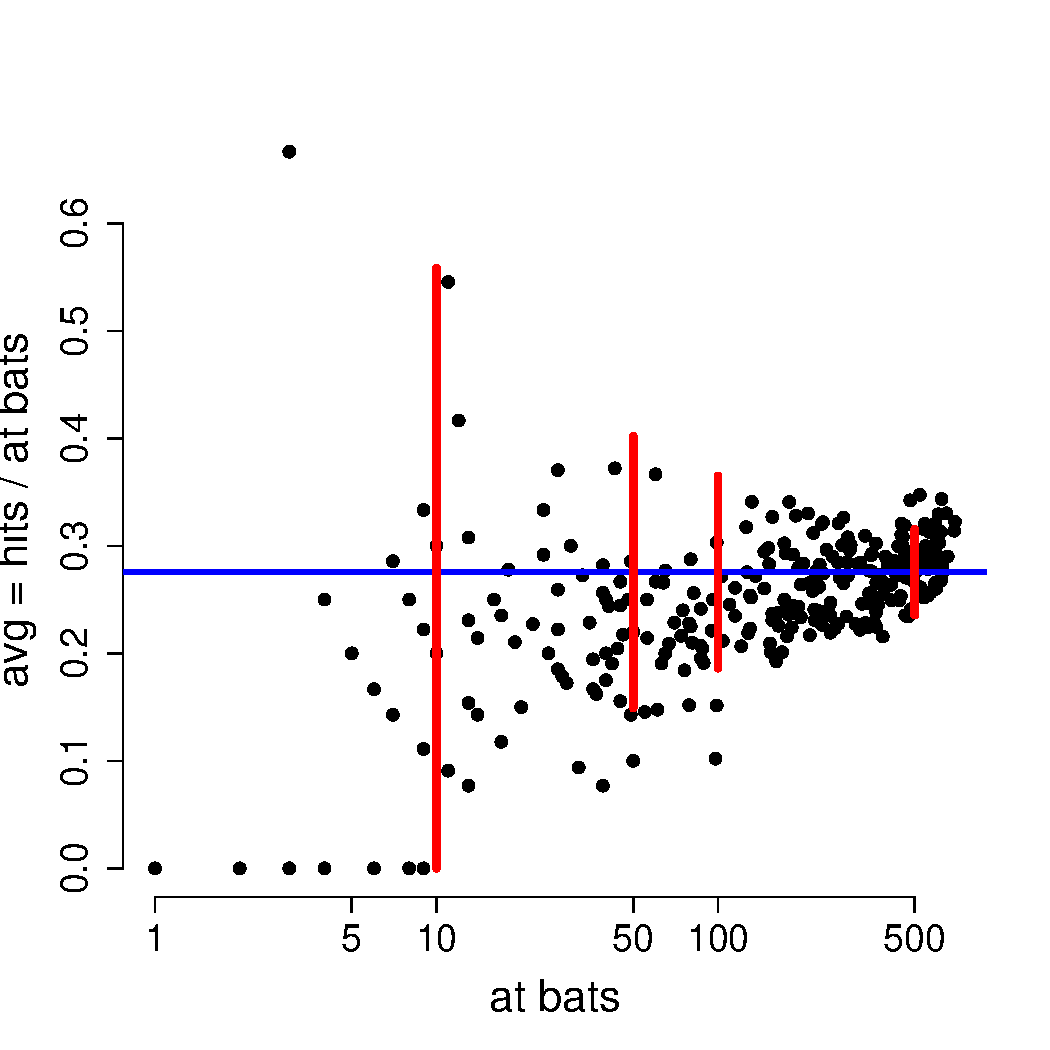
\includegraphics[height=1.4in]{img/bball-eda.pdf}
\end{center}
\end{minipage}

\sld{Pooling Data}
\begin{itemize}
\item How do we estimate the ability of a player who we observe
  getting 6 hits in 10 at-bats?  Or 0 hits in 5 at-bats?  Estimates of
  60\% or 0\% are absurd!
\item Same logic applies to players with 152 hits in 537 at bats.
\item \emph{No pooling}: estimate each player separately
\item \emph{Complete pooling}: estimate all players together (assume no difference
  in abilities)
\item \emph{Partial pooling}: somewhere in the middle
\begin{subitemize}
\item use information about other players (i.e., the population) 
to estimate a player's ability
\end{subitemize}
\end{itemize}

\sld{Hierarchical Models}
\begin{itemize}
\item Hierarchical models are principled way of determining how much
  pooling to apply.
\item Pull estimates toward the population mean based on amount of
  variation in population
\begin{subitemize}
\item low variance population: more pooling
\item high variance population: less pooling
\end{subitemize}
\item In limit
\begin{subitemize}
\item as variance goes to 0, get complete pooling
\item as variance goes to $\infty$, get no pooling
\end{subitemize}
\end{itemize}

\sld{Hierarchical Batting Ability}
\begin{itemize}
\item Instead of fixed priors, estimate priors along with other parameters
\item Still only uses data once for a single model fit
\item Data: $y_n, B_n$: hits, at-bats for player $n$
\item Parameters: $\theta_n$: ability for player $n$
\item Hyperparameters: $\alpha, \beta$: population mean and variance
\item Hyperpriors: fixed priors on $\alpha$ and $\beta$ (hardcoded)
\end{itemize}

\sld{Hierarchical Batting Model {\small (cont.)}}
\vspace*{-4pt}
\begin{eqnarray*}
y_n & \sim & \distro{Binomial}(B_n, \theta_n)
\\[4pt]
\theta_n & \sim & \distro{Beta}(\alpha,\beta)
\\[4pt]
\frac{\alpha}{\alpha + \beta} & \sim & \distro{Uniform}(0,1)
\\[4pt]
(\alpha + \beta) & \sim & \distro{Pareto}(1.5)
\end{eqnarray*}
\begin{itemize}
\item Sampling notation syntactic sugar for: \\[4pt]
{\footnotesize 
$
p(y,\theta,\alpha,\beta)
\ = \
\distro{Pareto}(\alpha + \beta | 1.5)
\,
\prod_{n=1}^N 
  \Big(
  \distro{Binomial}(y_n|B_n, \theta_n)
  \
  \distro{Beta}(\theta_n|\alpha,\beta) 
  \Big)
$
}
\item Pareto provides power law: \ \
{\small 
$
\distro{Pareto}(u|\alpha) \propto
\frac{\alpha}{u^{\alpha + 1}}
$
}
\item Should use more informative hyperpriors!
\end{itemize}

\sld{Hierarchical Prior Posterior}
\\[8pt]
\begin{minipage}[t]{0.55\textwidth}
\begin{itemize}
\item Draws from posterior (crosshairs at posterior mean)
\item Prior population mean:   0.271
\item Prior population scale:  400
\item Together yield prior std dev of 0.022
\item Mean is better estimated than scale (typical)
\end{itemize}
\end{minipage}
\begin{minipage}[t]{0.45\textwidth}
\vfill
\mbox{ } \ \ \ \ \ \ 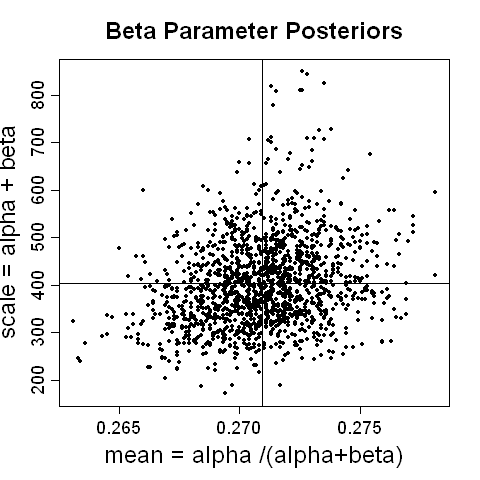
\includegraphics[height=1.4in]{img/baseball-beta-posterior-scatter.png}
\vfill
\end{minipage}

\sld{Posterior Ability {\normalsize (High Avg Players)}}
\\[8pt]
\begin{minipage}[t]{0.45\textwidth}
\begin{itemize}
\item Histogram of posterior draws for high-average players
\item Note uncertainty grows with lower at-bats
\\
\end{itemize}
\end{minipage}
\begin{minipage}[t]{0.55\textwidth}
\vfill
\mbox{ } \ \ \ \ \ \ 
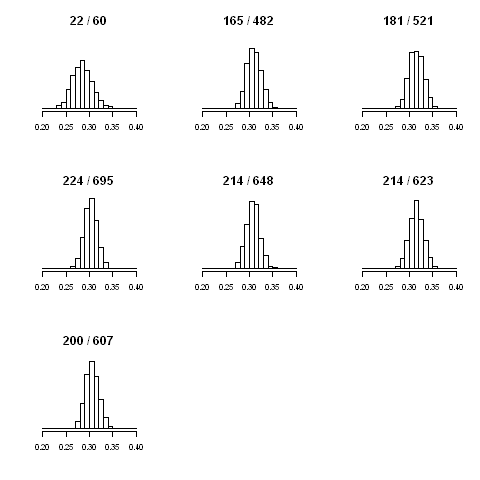
\includegraphics[height=1.95in]{img/batting-ability-posteriors.png}
\vfill
\end{minipage}

\sld{Multiple Comparisons}
\vspace*{-2pt}\small
\begin{itemize}
\item Who has the highest ability (based on this data)?
\item Probabilty player $n$ is best is 
\end{itemize}
%
\begin{center}
{\small
\begin{tabular}{rrr}
\emph{Average} & \emph{At-Bats} & $\Prob{\text{best}}$
\\ \hline
.347 & 521 & 0.12
\\
.343 & 623 & 0.11
\\
.342 & 482 & 0.08
\\
.330 & 648 & 0.04
\\
.330 & 607 & 0.04
\\
.367 & 60 & 0.02
\\
.322 & 695 & 0.02
\end{tabular}
}
\end{center}
\begin{itemize}
\item No clear winner---sample size matters.
\item In last game (of 162), Mauer (Minnesota) edged out Jeter (NY)
\end{itemize}


\sld{Bayesian ``Naive Bayes'' Four Ways}
\begin{itemize}
%
\item Joint Distribution \ $p(\pi,\phi,z,w)$, defined by:
\begin{subitemize}
\item $\pi \sim \mbox{\sf Dirichlet}(\alpha)$    \hfill (topic prevalence)
\item $\phi_k \sim \mbox{\sf Dirichlet}(\beta)$  \hfill (word
  prevalence in topic $k$)
\item $z_d \sim \mbox{\sf Categorical}(\pi)$     \hfill (topic for doc $d$)
\item $w_{d,n} \sim \mbox{\sf Categorical}(\phi_{z_d})$  \hfill (word
  $n$ in doc $d$)
\end{subitemize}
%
\item Inference Problems
\begin{subitemize}
\item fully supervised learning: \ $p(\pi,\phi \, | \, w, z)$
\item semi-supervised learning: \ $p(\pi, \phi \, | \, w, z, \ \tilde{w})$
\item unsupervised clustering: \ $p(\tilde{z} \, | \, \tilde{w})$
\item fully supervised prediction: \ $p(\tilde{z} \, | \, \tilde{w}, \ w, z)$
\item semi-supervised prediction: \ $p(\tilde{z} \, | \, \tilde{w}, \ w, z,
  \ \tilde{\tilde{w}})$
\end{subitemize}
\end{itemize}

\mypart{Warmup Exercise III}{Monte Carlo \\[8pt]\spc Integration}

\sld{Monte Carlo Calculation of $\pi$}

\noindent
\begin{minipage}[t]{0.65\textwidth}\small
\vspace*{2pt}
\begin{itemize}
\item Computing $\pi = 3.14\ldots$ via simulation is \emph{the} textbook application
of Monte Carlo methods.
\vfill
\item Generate points uniformly at random within the square
\item Calculate proportion within circle ($x^2 + y^2 < 1$) and multiply by square's area (4) to produce the area of the circle.
\item This area is $\pi$ (radius is 1, so area is $\pi r^2 = \pi$)
\end{itemize}
\end{minipage}
%
\begin{minipage}[t]{0.34\textwidth}
\vspace*{12pt}
\hfill 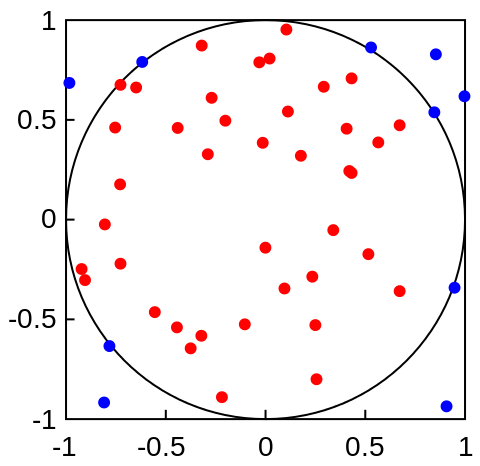
\includegraphics[height=1in]{img/mc-integration-wikipedia.png}
\\
\end{minipage}
\vfill
{ } \hfill {\tiny Plot by Mysid Yoderj courtesy of Wikipedia.}

\sld{Monte Carlo Calculation of $\pi$ {\normalsize (cont.)}}
%
\begin{itemize}
\item R code to calcuate $\pi$ with Monte Carlo simulation:
\\[-8pt]
{\small
\begin{Verbatim}
> x <- runif(1e6,-1,1)
> y <- runif(1e6,-1,1)

> prop_in_circle <- sum(x^2 + y^2 < 1) / 1e6

> 4 * prop_in_circle
[1] 3.144032
\end{Verbatim}
}
\end{itemize}

\sld{Accuracy of Monte Carlo}
\begin{itemize}
\item Monte Carlo is \emph{not} an approximation!
\item It can be made exact to within any $\epsilon$
\item Monte Carlo draws are i.i.d. by definition
\item Central limit theorem: expected error decreases at rate of
{\Large
\[
\frac{1}{\sqrt{N}}
\]
}
\item 3 decimal places of accuracy with 
sample size 1e6
\item Need $100 \times$ larger sample for each digit of accuracy
\end{itemize}

\sld{General Monte Carlo Integration}
\begin{minipage}[t]{0.69\textwidth}
\vspace*{-0.1in}
\small
\begin{itemize}
\item MC can calculate arbitrary definite integrals,
\[
\int_a^b f(x) \, dx
\]
\item Let $d$ upper bound $f(x)$ in $(a,b)$;  tightness determines
computational efficiency
\item Then generate random points uniformly in the rectangle bounded by $(a,b)$ and $(0,d)$
\item Multiply proportion of draws $(x,y)$ where $y < f(x)$ by area of rectangle, $d \times (b-a)$.
\item Can be generalized to multiple dimensions in obvious way
\end{itemize}
\end{minipage}
\begin{minipage}[t]{0.29\textwidth}
\mbox{ } \\
\mbox{ } \ \ \ \ 
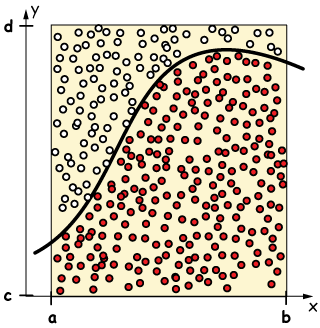
\includegraphics[height=0.9in]{img/monte-carlo-integration.png}
\end{minipage}
\vfill
\hfill
{\tiny Image courtesy of Jeff Cruzan, \url{http://www.drcruzan.com/NumericalIntegration.html}}

\sld{Monte Carlo for Expectations}
\begin{itemize}
\item Most quantities of interest are expectations
\item Suppose $f(\theta)$ is a function of random variable vector $\theta$
  \[
  \mathbb{E}[f(\theta)] = \int_{\Theta} f(\theta) \ p(\theta) \ d\theta.
  \]
where $\Theta$ is support of $p(\theta)$ (i.e., $\Theta =
\setcomp{\theta \, | \, p(\theta) > 0}$)
\item Generate samples $\theta^{(1)}, \theta^{(2)}, \ldots,
  \theta^{(M)}$ drawn from $p(\theta)$
\item Monte Carlo Estimator plugs in average for expectation:
  \[
  \mathbb{E}[f(\theta)|y] \approx \frac{1}{M} \sum_{m=1}^M f(\theta^{(m)})
  \]
\item This technique can be made as accurate as desired, because
\[
\mathbb{E}[f(\theta)] 
= 
\lim_{M \rightarrow \infty}
\frac{1}{M} \sum_{m=1}^M f(\theta^{(m)})
\]
\end{itemize}



\mypart{Part V}{Markov Chain \\[8pt]\spc{}Monte Carlo}

\sld{Markov Chain Monte Carlo}
%
\begin{itemize}
\item Standard Monte Carlo draws i.i.d. samples
\[
\theta^{(1)}, \ldots, \theta^{(M)}
\]
according to a probability function $p(\theta)$
\item Drawing i.i.d. samples is often impossible when
  dealing with complex densities like Bayesian posteriors $p(\theta|y)$
\item So we use Markov chain Monte Carlo (MCMC) in these cases and
  draw $\theta^{(1)}, \ldots, \theta^{(M)}$ from a Markov chain
\end{itemize}

\sld{Markov Chains}
\begin{itemize}
\item A Markov Chain is a sequence of random variables 
\[
\theta^{(1)},
  \theta^{(2)}, \ldots, \theta^{(M)}
\]
such that $\theta^{(m)}$ only depends on $\theta^{(m-1)}$, i.e.,
\[
p(\theta^{(m)} | y, \theta^{(1)}, \ldots, \theta^{(m-1)})
\ = \
p(\theta^{(m)} | y, \theta^{(m-1)})
\]
\item Drawing $\theta^{(1)}, \ldots, \theta^{(M)}$ from a Markov chain
  according to \\ $p(\theta^{(m)} \, | \, \theta^{(m-1)}, y)$ is more tractable
\item Require marginal of each draw, $p(\theta^{(m)}|y)$,
  to be equal to true posterior
\end{itemize}

\sld{Applying Markov Chain Monte Carlo}
\begin{itemize}
\item In practice, just like ordinary (non-Markov chain) Monte Carlo
\item Must adjust standard errors for dependence in Markov chain
\end{itemize}

\sld{MCMC for Posterior Mean}
\begin{itemize}
\item Standard Bayesian estimator is posterior mean
\[
\hat{\theta}  \ =  \ \int_{\Theta} \theta \, p(\theta|y) \, d\theta
\]
\begin{subitemize}
\item Posterior mean minimizes expected square error
\end{subitemize}
\item Estimate is a conditional expectation
\[
\hat{\theta} = \mathbb{E}[\theta|y]
\]
\item Compute by averaging
\[
\hat{\theta} \ \approx \ \frac{1}{M} \sum_{m=1}^M \theta
\]
\end{itemize}

\sld{MCMC for Posterior Variance}
\begin{itemize}
\item Posterior variance works the same way, given previous result
\[
\expectation{(\theta - \expectation{\theta})^2}
\approx \frac{1}{M} \sum_{m=1}^M (\theta^{(m)} - \hat{\theta})^2
\]
\end{itemize}

\sld{MCMC for Posterior Median}
\begin{itemize}
\item Alternative Bayesian estimator is posterior median
\begin{subitemize}
\item Posterior median minimizes expected absolute error
\end{subitemize}
\item Calculate as middle draw of $\theta^{(1)}, \ldots,
  \theta^{(M)}$
\begin{subitemize}
\item just sort and take halfway value
\item e.g., Stan shows 50\% point (or other quantiles)
\end{subitemize}
\end{itemize}

\sld{MCMC for Event Probability}
%
\begin{itemize}
\item Event probabilities are also expectations, e.g.,
\[
\Prob{\theta_1 > \theta_2}
\ = \ \expectation{\indicator{\theta_1 > \theta_2}}
\ = \ \int_{\Theta} \indicator{\theta_1 > \theta_2} \, p(\theta|y) d\theta.
\]
\item Estimation via MCMC just another plug-in:
\[
\Prob{\theta_1 > \theta_2} \approx 
\frac{1}{M} \sum_{m=1}^M \indicator{\theta_1^{(m)} > \theta_2^{(m)}}
\]
\item Again, can be made as accurate as necessary
\end{itemize}


\sld{Random-Walk Metropolis}
\begin{itemize}
\item Draw random initial parameter vector $\theta^{(1)}$ (in
  support) 
\item For $m \in \range{2}{M}$
\hspace*{-8pt}
\begin{subitemize}
\item Sample proposal from a (symmetric) jumping distribution, e.g.,
\[
\theta^*
\ \sim \ 
\distro{MultiNormal}(\theta^{(m-1)}, \ \sigma \mbox{\bfseries I})
\]
where {\bfseries I} is the identity matrix
\item 
\vspace*{4pt}
Draw $u^{(m)} \sim \distro{Uniform}(0,1)$ and set
\[
\theta^{(m)} 
\ = \
\begin{cases}
\theta^{*} 
  & \text{if } u^{(m)} < {\displaystyle \frac{p(\theta^{*}|y)}{p(\theta^{(m)}|y)}}
\\[8pt]
\theta^{(m-1)}
  & \text{otherwise}
\end{cases}
\]
\end{subitemize}
\end{itemize}

\sld{Metropolis and Normalization}
\begin{itemize}\small
\item Metropolis only uses posterior in a ratio:
\[
\frac{p(\theta^{*} \, | \, y)}
     {p(\theta^{(m)} \, | \, y)}
\]
\item This \myemph{allows} the use of \myemph{unnormalized densities}
\item Recall Bayes's rule:
\[
p(\theta | y) \propto p(y|\theta) \, p(\theta)
\]
\item Thus we only need to evaluate sampling (likelihood) and prior
\item It also sidesteps computing the normalizing term
\[
\int_{\Theta} p(y|\theta) \, p(\theta) d\theta
\]
\end{itemize}

\sld{Metropolis-Hastings}
\begin{itemize}
\item Generalizes Metropolis to asymmetric proposals
\item Acceptance ratio is
\[
\frac{J(\theta^{(m)}|\theta^{*}) \ \times \ p(\theta^{*}|y)}
     {J(\theta^{*}|\theta^{(m-1)}) \ \times \ p(\theta^{(m)}|y)}
\]
where $J$ is the (potentially asymmetric) proposal density
\item i.e., 
{\small
\[
\frac{\mbox{probabilty of being at } \theta^*
      \mbox{ and jumping to } \theta^{(m-1)}}
     {\mbox{probability of being at } \theta^{(m-1)}
      \mbox{ and jumping to } \theta^{*}}
\]
}
\end{itemize}

\sld{Metropolis-Hastings (cont.)}
\begin{itemize}
\item General form ensures equilibrium 
  by maintaining \emph{detailed balance}
\item Like Metropolis, only requires ratios
\item Many algorithms involve a Metropolis-Hastings ``correction''
\end{itemize}

\sld{Optimal Proposal Scale?}
%
\begin{itemize}\small
\item Proposal scale $\sigma$ is a free; too low or high is inefficient
\begin{center}
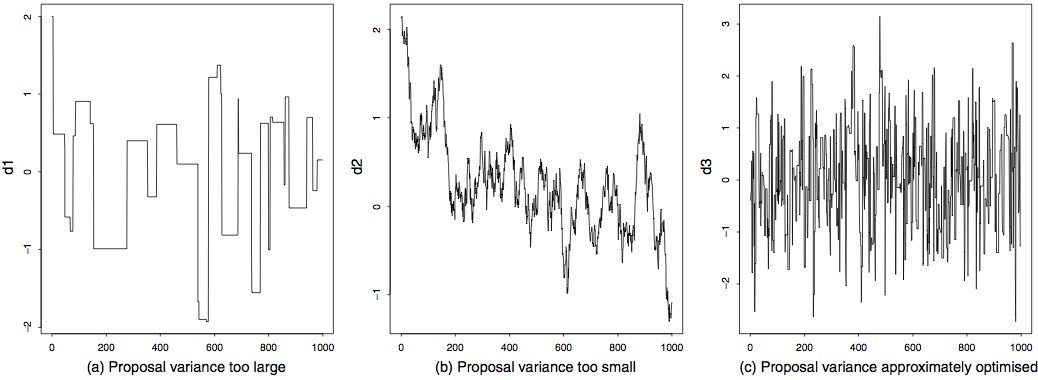
\includegraphics[width=0.85\textwidth]{img/roberts-rosenthal-traceplots.jpg}
\end{center}
\item \emph{Traceplots} show parameter value on $y$ axis, iterations on $x$
\item Empirical tuning problem; theoretical optima exist for some
  cases
\end{itemize}
\vfill\hfill
{\tiny Roberts and Rosenthal (2001) Optimal Scaling for Various
  Metropolis-Hastings Algorithms. {\slshape Statistical Science}.}


\sld{Convergence}
\begin{itemize}
\item Imagine releasing a hive of bees in a sealed house
\begin{subitemize}
\item they disperse, but eventually reach equilibrium where the same
  number of bees leave a room as enter it (on average)
\end{subitemize}
\item May take many iterations for Markov chain to reach equilibrium
\end{itemize}

\sld{Convergence: Example}
\begin{center}
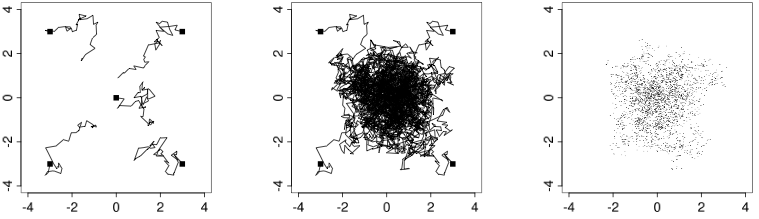
\includegraphics[width=0.8\textwidth]{img/bda-diffuse-converge.png}
\end{center}
\begin{itemize}
\item Four chains with different starting points
\begin{subitemize}
\item \emph{Left}: 50 iterations
\item \emph{Center}: 1000 iterations
\item  \emph{Right}: Draws from second half of each chain
\end{subitemize}
\vfill\hfill {\footnotesize Gelman et al., {\slshape Bayesian Data Analysis}}
\end{itemize}


\sld{Potential Scale Reduction ($\hat{R}$)}
\begin{itemize}
\item Gelman \& Rubin recommend $M$ chains of $N$ draws with
  \myemph{diffuse initializations}
\item Measure that each chain has same posterior mean and variance
\item If not, may be stuck in multiple modes or just not converged yet
\item Define statistic $\hat{R}$ of chains s.t. \myemph{at convergence},
$\hat{R} \rightarrow 1$
\begin{subitemize}
\item $\hat{R} >\!> 1$ implies non-convergence
\item $\hat{R} \approx 1$ \myemph{does not guarantee convergence}
\item Only measures marginals
\end{subitemize}
\end{itemize}

\sld{Split $\hat{R}$}
\begin{itemize}
\item Vanilla $\hat{R}$ may not diagnose non-stationarity
\begin{subitemize}
\item e.g., a sequence of chains with an increasing parameter
\end{subitemize}
\item \myemph{Split $\hat{R}$}: \ Stan splits each chain into first and
  second half
\begin{subitemize}
\item start with $M$ Markov chains of $N$ draws each
\item split each in half to creates $2M$ chains of $N/2$ draws
\item then apply $\hat{R}$ to the $2M$ chains
\end{subitemize}
\end{itemize}


\sld{Calculating $\hat{R}$ Statistic: Between}
\begin{itemize}
\item \myemph{Between-sample variance} estimate
\[\textstyle
B
= \frac{N}{M-1} \, \sum_{m=1}^M (\bar{\theta}^{(\bullet)}_{m} - \bar{\theta}^{(\bullet)}_{\bullet})^2,
\]
%
where
%
\[\textstyle
\bar{\theta}_m^{(\bullet)}
= \frac{1}{N} \sum_{n = 1}^N \theta_m^{(n)}
\ \ \ \ \
\mbox{and}
\ \ \ \ \
\bar{\theta}^{(\bullet)}_{\bullet}
= \frac{1}{M} \, \sum_{m=1}^M \bar{\theta}_m^{(\bullet)}.
\]
\end{itemize}

\sld{Calculating $\hat{R}$ (cont.)}
\begin{itemize}
\item \myemph{Within-sample variance} estimate:
\[\textstyle
W 
= \frac{1}{M} \, \sum_{m=1}^M s_m^2,
\]
where
\[\textstyle
s_m^2 = \frac{1}{N-1} \, \sum_{n=1}^N (\theta^{(n)}_m - \bar{\theta}^{(\bullet)}_m)^2.
\]
\end{itemize}

\sld{Calculating $\hat{R}$ Statistic (cont.)}
\begin{itemize}
\item \myemph{Variance} estimate:
\[\textstyle
\widehat{\mbox{var}}^{+}\!(\theta|y)
= \frac{N-1}{N}\, W \, + \, \frac{1}{N} \, B.
\]
\\[4pt]
recall that $W$ is within-chain variance and $B$ between-chain
%
\vspace*{6pt}
\item \myemph{Potential scale reduction} statistic (``R hat'')
\[\textstyle
\hat{R} 
\, = \,
\sqrt{\frac{\widehat{\mbox{var}}^{+}\!(\theta|y)}{W}}.
\]
\end{itemize}


\sld{Correlations in Posterior Draws}
%
\begin{itemize}
\item Markov chains typically display autocorrelation in the series of
  draws $\theta^{(1)}, \ldots, \theta^{(m)}$
\item Without i.i.d. draws, central limit theorem \emph{does not apply}
\item Effective sample size $N_{\mbox{\footnotesize eff}}$ divides out
  autocorrelation
\item $N_{\mbox{\footnotesize eff}}$ must be estimated from sample
\begin{subitemize}
\item Fast Fourier transform computes correlations at all lags
\end{subitemize}
\vspace*{-6pt}
\item Estimation accuracy proportional to 
{\large
\[
\frac{1}{\sqrt{N_{\mbox{\small eff}}}}
\]
}
\end{itemize}

\sld{Reducing Posterior Correlation}
\begin{itemize}
\item Tuning algorithm parameters to ensure good mixing
\item Recall Metropolis traceplots of Roberts and Rosenthal:
\begin{center}
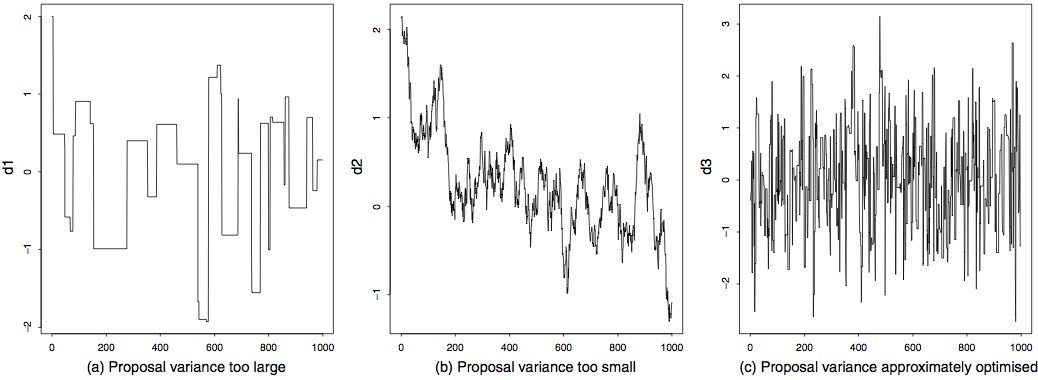
\includegraphics[width=0.85\textwidth]{img/roberts-rosenthal-traceplots.jpg}
\end{center}
\item Good jump scale $\sigma$ produces good mixing and high
$N_{\mbox{\footnotesize eff}}$
\end{itemize}


\sld{Effective Sample Size (ESS)}
%
\begin{itemize}
\item Autocorrelation at lag $t$ is correlation between subsequences
\begin{subitemize}
\item $(\theta^{(1)},\ldots, \theta^{(N-t)})$ and $(\theta^{(1 + t)}, \ldots, \theta^{(N)})$
\end{subitemize}
\item  Suppose chain has density $p(\theta)$ with
\begin{subitemize}
\item $\mathbb{E}[\theta] = \mu$ \ \ and \ \ $\mbox{\rm Var}[\theta] = \sigma^2$ 
\end{subitemize}
\item Autocorrelation $\rho_t$ at lag $t \geq 0$:
\[
\rho_t  =  \frac{1}{\sigma^2} \, \int_{\Theta} (\theta^{(n)} - \mu)
       (\theta^{(n+t)} - \mu) \, p(\theta) \, d\theta
\]
\item Because $p(\theta^{(n)}) = p(\theta^{(n+t)}) = p(\theta)$ at convergence,
\[
\rho_t = \frac{1}{\sigma^2} \, \int_{\Theta} \theta^{(n)} \, \theta^{(n+t)} \, p(\theta) \, d\theta
\]
\end{itemize}

\sld{Estimating Autocorrelations}
\begin{itemize}\small
\item Effective sample size is defined by
\[
N_{\mbox{\scriptsize eff}}
\ = \
\frac{N}{\sum_{t = -\infty}^{\infty} \rho_t}
\ = \
\frac{N}{1 + 2 \sum_{t = 1}^{\infty} \rho_t}
\]
\item Estimate in terms of variograms at lag $t$ (calc with FFT),
\[
V_t = 
\frac{1}{M}
\,
\sum_{m=1}^M 
\
\left(
\frac{1}{N_m - t}
\sum_{n=t+1}^{N_m}
\left(
\theta_m^{(n)} - \theta_m^{(n-t)}
\right)^2
\right)
\]
\item Adjust autocorrelation at lag $t$ using cross-chain variance
  as
\[
\hat{\rho}_t
= 1 - \frac{\displaystyle V_t}{
            \displaystyle 2 \, \widehat{\mbox{var}}^{+}}
\]
\item If not converged, $\widehat{\mbox{var}}^{+}$ overestimates variance
\end{itemize}

\sld{Estimating $N_{\normalsize eff}$}
\begin{itemize}
\item Let $T'$ be first lag s.t.\ $\rho_{T' + 1} < 0$, 
\item Estimate autocorrelation by
\[
\hat{N}_{\mbox{\scriptsize eff}}
= 
\frac{MN}
     {1 + \sum_{t=1}^{T'} \hat{\rho}_t}.
\]
\item NUTS avoids negative autocorrelations, so first negative
  autocorrelation estimate is reasonable
\vfill
\item See {\footnotesize Charles Geyer (2013) Introduction to MCMC. In
    {\slshape Handbook of MCMC}.
 (free online at \url{http://www.mcmchandbook.net/index.html})}
\end{itemize}


\sld{Gibbs Sampling}
\begin{itemize}
\item Draw random initial parameter vector $\theta^{(1)}$ (in
  support) 
\item For $m \in \range{2}{M}$
\begin{subitemize}
\item For $n \in \range{1}{N}$:
\begin{itemize}
\item draw 
$\theta^{(m)}_n$ according to conditional \\[8pt]
$p(\theta_n|\theta_1^{(m)},\ldots,\theta_{n-1}^{(m)}, \, \theta_{n+1}^{(m-1)},
\ldots,\theta_N^{(m-1)},  y)$.
\end{itemize}
\end{subitemize}
\item e.g, with $\theta = (\theta_1,\theta_2,\theta_3)$:
\begin{subitemize}
\item draw \ $\theta_1^{(m)}$  \ according to \ $p(\theta_1 | \theta_2^{(m-1)},
  \theta_3^{(m-1)}, y)$
\item draw \ $\theta_2^{(m)}$ \ according to \ $p(\theta_2 | \theta_1^{(m)},
  \theta_3^{(m-1)}, y)$
\item draw \ $\theta_3^{(m)}$ \ according to \ $p(\theta_3 | \theta_1^{(m)},
  \theta_2^{(m)}, y)$
\end{subitemize}
\end{itemize}

\sld{Generalized Gibbs}
\begin{itemize}
\item ``Proper'' Gibbs requires the conditional Monte Carlo draws
\begin{subitemize}
\item typically works only for conjugate priors
\end{subitemize}
\item In general case, may need to use less efficient conditional
  draws
\begin{subitemize}
\item Slice sampling is a popular general technique that works for
  discrete or continuous $\theta_n$
\item Adaptive rejection sampling is another alternative
\item Very difficult in more than one or two dimensions
\end{subitemize}
\end{itemize}

\sld{Sampling Efficiency}
\begin{itemize}
\item We care only about $N_{\mbox{\footnotesize eff}}$ per second
\item Decompose into
{\small
\begin{enumerate}
\item Iterations per second
\item Effective samples per iteration
\end{enumerate}
}
\item Gibbs and Metropolis have high iterations per second (especially
  Metropolis)
\item But they have low effective samples per iteration (especially
  Metropolis) 
\item Both are particular weak when there is high correlation among
  the parameters in the posterior
\end{itemize}

\sld{Hamiltonian Monte Carlo \& NUTS}
\begin{itemize}
\item Slower iterations per second than Gibbs or Metropolis
\item Much higher number of effective samples per iteration for
complex posteriors (i.e., high curvature and correlation)
\item Overall, much higher $N_{\mbox{\footnote eff}}$ per second
\vfill
\item Details in the next talk \ldots
\item Along with details of how Stan implements HMC and NUTS
\end{itemize}

\mypart{}{The End}

\sld{Why Stan?}
%
\begin{itemize}
\item {\slshape\bfseries Application}: Fit rich Bayesian statistical models
\end{itemize}
%
\vspace*{2pt}
\begin{itemize}
\item {\slshape Problem}: Gibbs and Metropolis too slow (diffusive) 
\item {\slshape Solution}: Hamiltonian Monte Carlo (flow)
%
\vspace*{8pt}
\item {\slshape Problem}:  Interpreters slow and unscalable
\item {\slshape Solution}: Compiled to C++
%
\vspace*{8pt}
\item {\slshape Problem}:  Need gradients of log posterior for HMC
\item {\slshape Solution}: Reverse-mode algorithmic differentation
\end{itemize}

\sld{Why? (cont.)}
%
\begin{itemize}
\item {\slshape Problem}:  Existing algo-diff slow, limited, unextensible
\item {\slshape Solution}: Our own algo-diff
%
\vspace*{8pt}
\item {\slshape Problem}:  Algo-diff requires functions templated on
  all args
\item {\slshape Solution}: Our own density library, Eigen linear
 algebra
%
\vspace*{8pt}
\item {\slshape Problem}:  Need unconstrained parameters for HMC
\item {\slshape Solution}: Variable transforms w. Jacobian determinants
%
\end{itemize}

\sld{Why? (cont.)}
%
\begin{itemize}
\item {\slshape Problem}:  Need ease of use of BUGS
\item {\slshape Solution}: Compile a domain-specific language
%
\vspace*{8pt}
\item {\slshape Problem}:  Pure directed graphical language inflexible
\item {\slshape Solution}: Imperative probabilistic programming
  language
\vspace*{8pt}
\item {\slshape Problem}:  Need to tune parameters for HMC
\item {\slshape Solution}: Tune step size and estimate mass matrix
  during warmup;  on-the-fly number of steps (NUTS)
%
\end{itemize}

\sld{Why? (cont.)}
\begin{itemize}
%
\vspace*{8pt}
\item {\slshape Problem}:  Efficient up-to-proportion density calcs
\item {\slshape Solution}: Density template metaprogramming 
%
\vspace*{8pt}
\item {\slshape Problem}:  Limited error checking, recovery
\item {\slshape Solution}: Static model typing, informative exceptions
%
\vspace*{8pt}
\item {\slshape Problem}:  Poor numerical stability
\item {\slshape Solutions}:
Taylor expansions, e.g., {\small \code{log1p()}}
\\[2pt]
compound functions, e.g., {\small \code{log\_sum\_exp()}, \
\code{BernoulliLogit()}}
\\[2pt]
limits at boundaries, e.g., {\small \code{multiply\_log()}}

\end{itemize}

\sld{Why? (continued)}
\begin{itemize}
\item {\slshape Problem}:  Nobody knows everything
\item {\slshape Solution}: Expand project team with specialists
\vspace*{8pt}
\item {\slshape Problem}:  Expanding code and project team
\item {\slshape Solution}: GitHub: branch, pull 
  request, code review
\item {\slshape Solution}: Jenkins: continuous integration
\item {\slshape Solution}: ongoing refactoring and code simplification
%
\end{itemize}

\sld{Why? (continued)}
\begin{itemize}
\item {\slshape Problem}:  Heterogeneous user base
\item {\slshape Solution}: More interfaces (R, Python, MATLAB, Julia)
\item {\slshape Solution}:  domain-specific examples, tutorials
\vspace*{8pt}
\item {\slshape Problem}:  Restrictive licensing limits use
\item {\slshape Solution}: Code and doc open source
(BSD, CC-BY)
\end{itemize}

\sld{What is Stan?}

\begin{itemize}
\item Stan is an \myemph{imperative} probabilistic programming language
\vspace*{-12pt}
  \begin{subitemize}
  \item  cf., BUGS: declarative; \ Church: functional; \ Figaro: object-oriented
  \end{subitemize}
\item Stan \myemph{program}
  \begin{subitemize}
  \item declares data and (constrained) parameter variables
  \item defines log posterior (or penalized likelihood)
  \end{subitemize}
\item Stan \myemph{inference}
  \begin{subitemize}
  \item MCMC for full Bayesian inference
  \item VB for approximate Bayesian inference
  \item MLE for penalized maximum likelihood estimation
  \end{subitemize}
\end{itemize}

\sld{Platforms and Interfaces}
\vspace*{-2pt}
\begin{itemize}
\item \myemph{Platforms}:  Linux, Mac OS X, Windows
\item \myemph{C++ API}: {\small portable, standards compliant (C++03)}
\item \myemph{Interfaces}
  \begin{subitemize}\footnotesize
  \item \myemph{CmdStan}: Command-line or shell interface (direct executable)
  \item \myemph{RStan}: R interface (Rcpp in memory)
  \item \myemph{PyStan}: Python interface (Cython in memory)
  \item \myemph{MatlabStan}: MATLAB interface (external process)
  \item \myemph{Stan.jl}: Julia interface (external process)
  \item \myemph{StataStan}: Stata interface (external process)
      [under testing]
    \end{subitemize}
\item \myemph{Posterior Visualization \& Exploration}
\begin{subitemize}
 \item \myemph{ShinyStan}: Shiny (R) web-based
\end{subitemize}
\end{itemize}
\vfill


\sld{Who's Using Stan?}
\begin{itemize}
\item 1200 \myemph{users group} registrations;  10,000 manual
  \myemph{downloads} (2.5.0); 300 Google scholar citations (100+ fitting)
\item \myemph{Biological sciences}: {\footnotesize
clinical drug trials, entomology, opthalmology,
neurology, genomics, agriculture, botany, fisheries,
cancer biology, epidemiology, population ecology, neurology
}
\item \myemph{Physical sciences}: {\footnotesize 
astrophysics, molecular biology, oceanography, climatology
}
\item \myemph{Social sciences}: {\footnotesize
 population dynamics, psycholinguistics, social networks, political science
}
\item \myemph{Other}: {\footnotesize materials engineering, finance, actuarial,
  sports, public health, recommender systems, educational testing}
\end{itemize}

\sld{Documentation}
% 
\begin{itemize}
\item {\slshape Stan User's Guide and Reference Manual}
\begin{subitemize}
\item 500+ pages
\item Example models, modeling and programming advice
\item Introduction to Bayesian and frequentist statistics 
\item Complete language specification and execution guide
\item Descriptions of algorithms (NUTS, R-hat, n\_eff)
\item Guide to built-in distributions and functions
\end{subitemize}
\item Installation and getting started manuals by interface
\begin{subitemize}
\item RStan, PyStan, CmdStan, MatlabStan, Stan.jl
\item RStan vignette
\end{subitemize}
\end{itemize}

\sld{Books and Model Sets}
\begin{itemize}
\item \myemph{Model Sets} Translated to Stan
\begin{subitemize}
\item BUGS and JAGS examples (most of all 3 volumes) 
\item Gelman and Hill (2009) {\slshape Data Analysis Using Regression and
    Multilevel/Hierarchical Models}
\item Wagenmakers and Lee (2014) {\slshape Bayesian Cognitive Modeling}
\end{subitemize}
\item \myemph{Books} with Sections on Stan
\begin{subitemize}
\item Gelman et al. (2013) {\slshape Bayesian Data Analysis}, 3rd Edition.
\item Kruschke (2014) {\slshape Doing Bayesian Data Analysis, Second
    Edition: A Tutorial with R, JAGS, and Stan}
\item Korner-Nievergelt et al. (2015) {\slshape Bayesian Data Analysis in
    Ecology Using Linear Models with R, BUGS, and Stan}
\end{subitemize}
\end{itemize}

\sld{Scaling and Evaluation}
\begin{center}
\vspace*{-6pt}
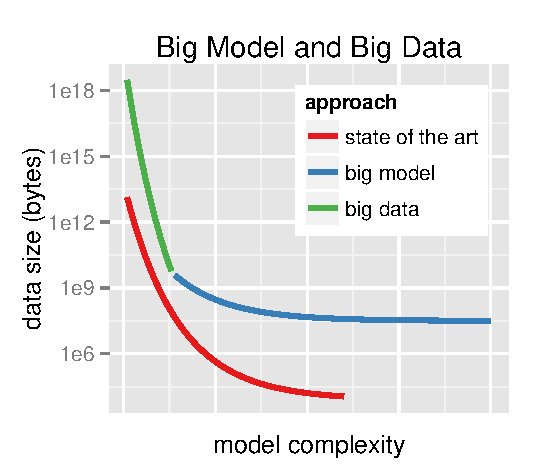
\includegraphics[width=0.4\textwidth]{img/big-model-big-data.pdf}
\vspace*{-6pt}
\end{center}
\begin{itemize}
\item Types of Scaling: data, parameters, \myemph{models}
\item Time to converge and per effective sample size: \\[2pt]
\mbox{ } \ \ \ {0.5--{\large$\infty$} times faster than BUGS \& JAGS}
\item Memory usage: \ {1--10\% of BUGS \& JAGS}
\end{itemize}


\sld{NUTS vs.\ Gibbs and Metropolis}

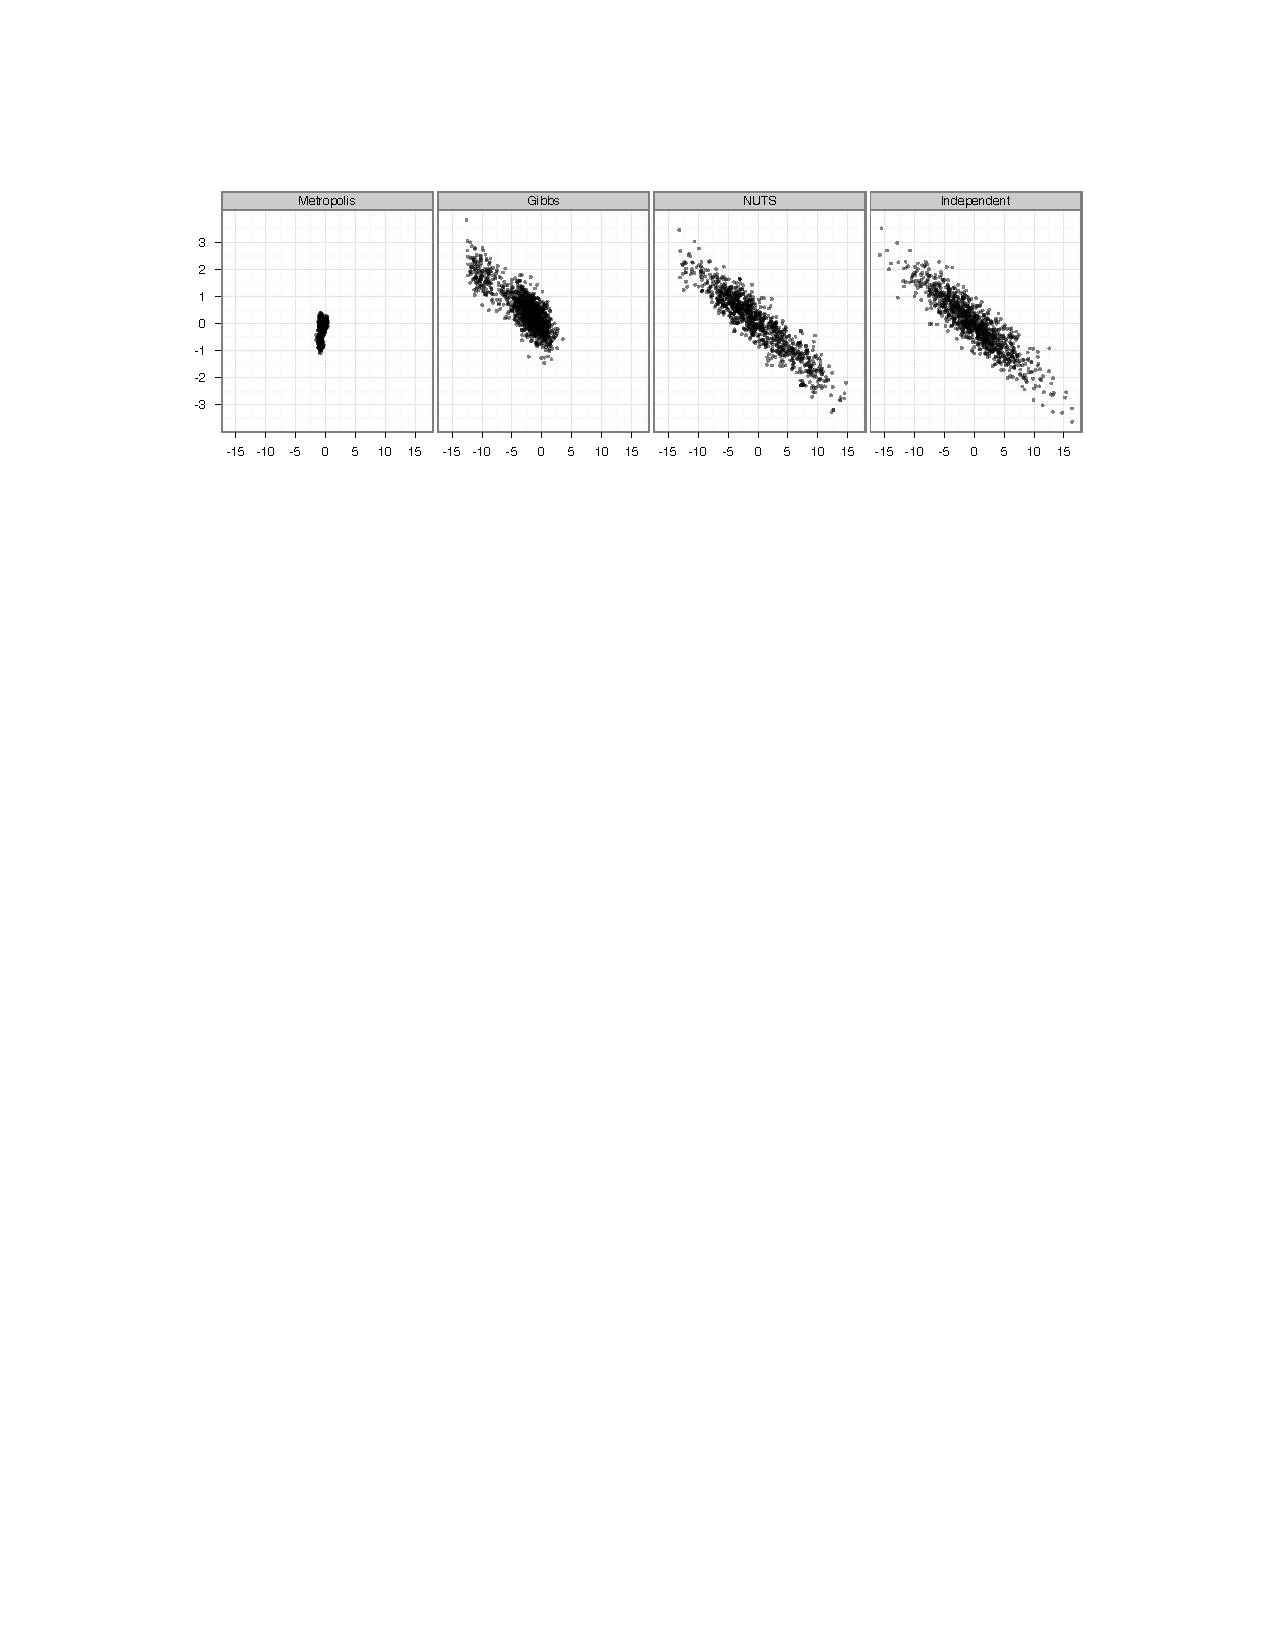
\includegraphics[width=0.9\textwidth]{img/nuts-vs.pdf}
\begin{subitemize}
\item Two dimensions of highly correlated 250-dim normal
\item \myemph{1,000,000 draws} from Metropolis and Gibbs (thin to 1000)
\item \myemph{1000 draws} from NUTS; 1000 independent draws
\end{subitemize}

\sld{Stan's Autodiff vs.\ Alternatives}

\begin{subitemize}
\item Among \myemph{C++ open-source} offerings: 
Stan is \myemph{fastest} (for gradients), 
\myemph{most general} (functions supported), 
and \myemph{most easily extensible} (simple OO)
\end{subitemize}
\vspace*{-8pt}
\hfill
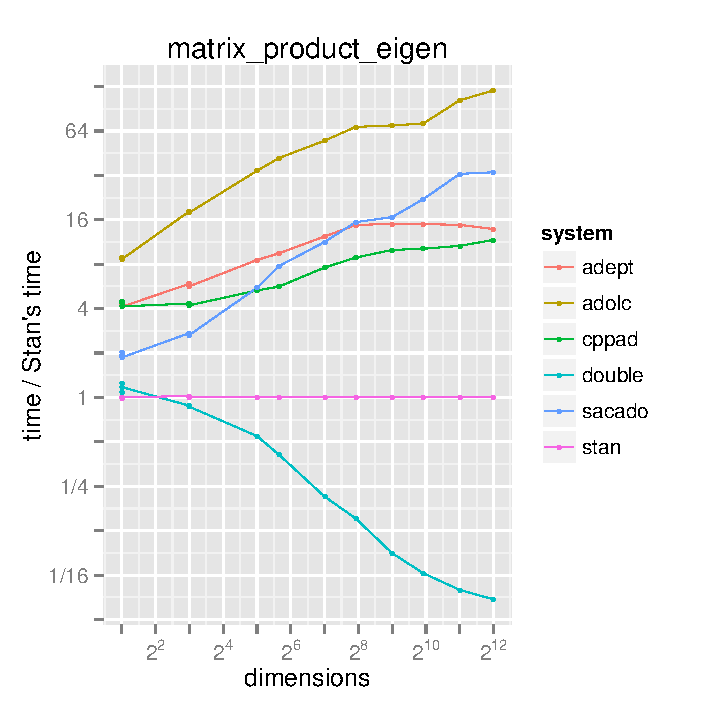
\includegraphics[width=0.45\textwidth]{img/autodiff-eval-matrix-product-eigen.pdf}
\hfill
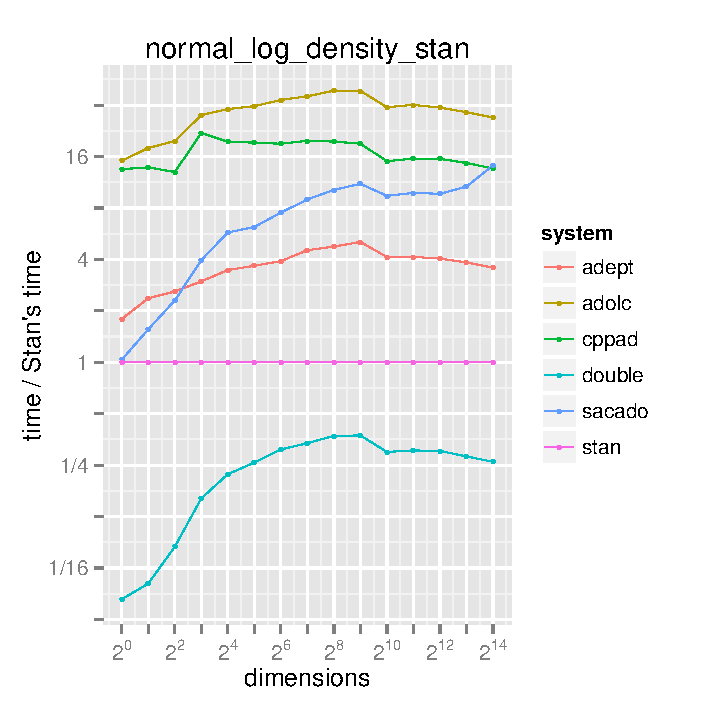
\includegraphics[width=0.45\textwidth]{img/autodiff-eval-normal-density.pdf}
\hfill


\mypart{Part I}{Stan Front End}


\sld{Estimating a Proportion}
\vspace*{3pt}
\begin{subitemize}
\item \myemph{Prior}: \ $\theta \sim \distro{Uniform}(0,1)$
\hfill $\theta \in (0,1)$
\item \myemph{Likelihood}: \ $y_n \sim \distro{Bernoulli}(\theta)$ for
  $n \in 1{:}N$
\hfill $y_n \in \setcomp{0,1}$
%
\item \myemph{Joint}:
\vspace*{-12pt}
\begin{eqnarray*}
\textstyle
\hspace*{24pt} p(y,\theta) & = & p(\theta) \times p(y \, | \, \theta)
\\[8pt]
& = & \textstyle p(\theta) \times \prod_{n=1}^N p(y_n \, | \, \theta)
\\[8pt]
& = &  \textstyle \distro{Uniform}(\theta \, | \, 0, 1)
                  \times \prod_{n=1}^N \distro{Bernoulli}(y_n | \theta)
\end{eqnarray*}
%
\vspace*{-8pt}
where
\vspace*{6pt}
\[
\distro{Bernoulli}(y_n \, | \, \theta) \ = \
\begin{cases}
\theta & \mbox{if } y_n = 1
\\
(1 - \theta) & \mbox{if } y_n = 0
\end{cases}
\]
and
\[
\distro{Uniform}(\theta \, | \, 0,1) \ = \ 1
\]
\end{subitemize}

\sld{Estimating a Proportion in Stan}
\vfill
\spc
\begin{minipage}[t]{0.8\textwidth}\small
\begin{Verbatim}
data {
  int<lower=0> N;
  int<lower=0, upper=1> y[N];
}
parameters {
  real<lower=0, upper=1> theta;
} 
model {
  y ~ bernoulli(theta);
}
\end{Verbatim}
\end{minipage}

\sld{Default Priors and Vectorization}
\begin{itemize}
\item All parameters are uniform on constrained values by default
\item Probability functions can be vectorized (more efficient)
\item Thus
{\small
\begin{Verbatim}
      y ~ bernoulli(theta);
\end{Verbatim}
}
\mbox{ }
\\
{\normalsize has the same behavior as}
\\
{\small
\begin{Verbatim}
      theta ~ uniform(0,1);
      for (n in 1:N) 
        y[n] ~ bernoulli(theta);
\end{Verbatim}
}
\end{itemize}


\sld{Maximum (Penalized) Likelihood}

\begin{center}
\begin{minipage}[t]{0.8\textwidth}\small
\begin{Verbatim}
> library(rstan);
> N <- 5;
> y <- c(0,1,1,0,0);
> model <- stan_model("bernoulli.stan");
> mle <- optimizing(model, data=c("N", "y"));
...
> print(mle, digits=2)
$par              $value  (log density)
theta             [1] -3.4
  0.4 
\end{Verbatim}
\begin{subitemize}
\item Posterior: $\distro{Beta}(1+2, 1+3)$;  mode $0.40$; mean $0.43$
\item Density: MLE w/o Jacobian;  MCMC with Jacobian
\end{subitemize}
\end{minipage}
\end{center}


\sld{Bayesian Posterior}

\begin{minipage}[t]{\textwidth}
\footnotesize
\begin{Verbatim}
> N <- 5;   y <- c(0,1,1,0,0);
> fit <- stan("bernoulli.stan", data = c("N", "y"));
> print(fit, digits=2)
\end{Verbatim}
%
\vspace*{1pt}
%
\begin{Verbatim}[fontshape=sl]
Inference for Stan model: bernoulli.
4 chains, each with iter=2000; warmup=1000; thin=1; 

        mean    se    sd   2.5%    50%  97.5%  n_eff  Rhat
theta  0.43  0.01  0.18   0.11   0.42   0.78   1229     1
lp__  -5.33  0.02  0.80  -7.46  -5.04  -4.78   1201     1
\end{Verbatim}
%
\vspace*{3pt}
%
\begin{Verbatim}
> hist( extract(fit)$theta )
\end{Verbatim}
\vspace*{-24pt}
\hfill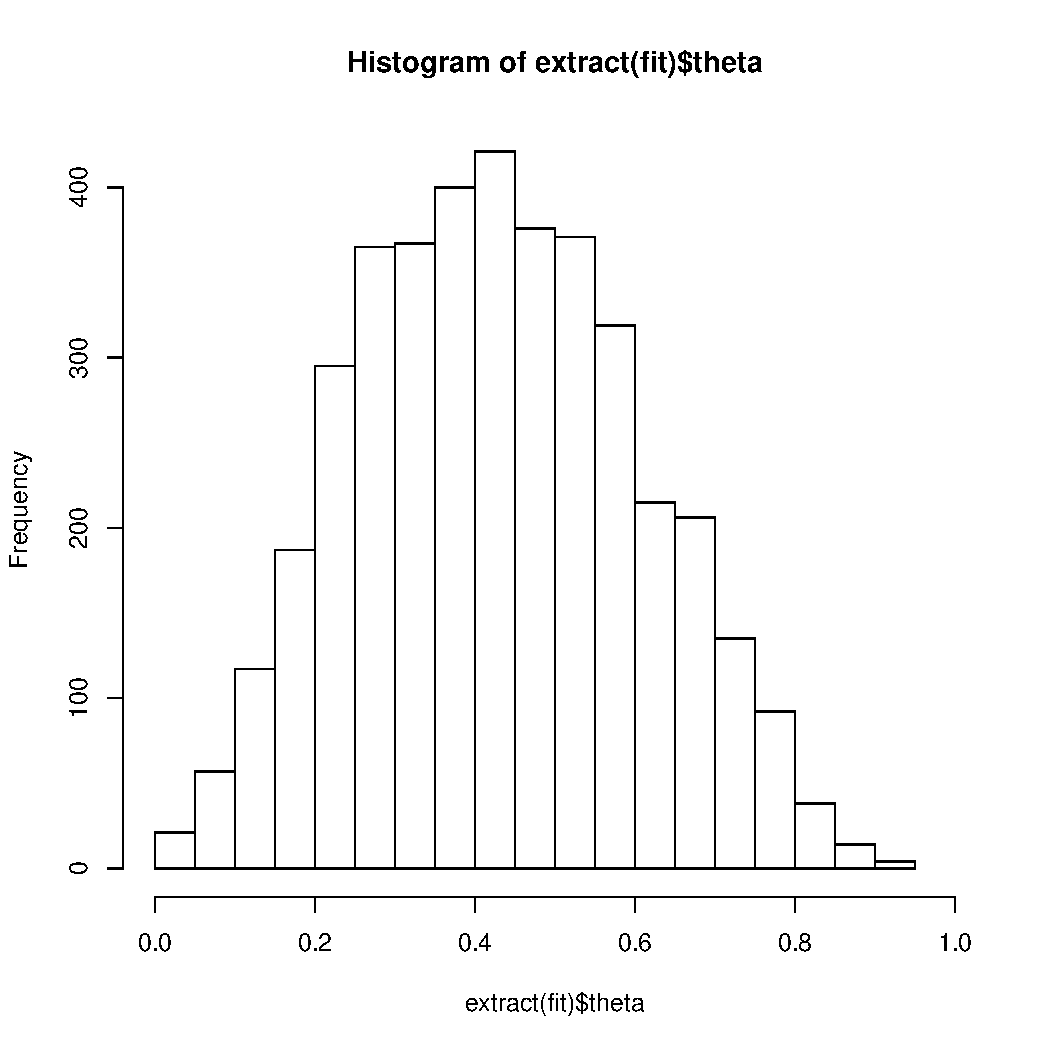
\includegraphics[height=0.9in]{img/bernoulli-posterior-histo.pdf}
\hspace*{24pt}
\end{minipage}


\sld{Linear Regression (Normal Noise)}
\begin{itemize}
\item \myemph{Likelihood}:
\begin{subitemize}
\item  $y_n = \alpha + \beta \, x_n + \epsilon_n$
\item  $\epsilon_n \sim \mbox{Normal}(0,\sigma)$ \hfill for $n \in 1{:}N$
\end{subitemize}
\item Equivalently,
\begin{subitemize}
\item  $y_n \sim \distro{Normal}(\alpha + \beta \, x_n, \, \sigma)$
\end{subitemize}
\item \myemph{Priors} (improper)
\begin{subitemize}
\item $\sigma \sim \distro{Uniform}(0,\infty)$
\item $\alpha, \beta \sim \distro{Uniform}(-\infty, \infty)$
\end{subitemize}
\item Stan allows \myemph{improper prior}; requires \myemph{proper posterior}.
\end{itemize}

\sld{Linear Regression in Stan}

{\footnotesize
\begin{Verbatim}
     data {
       int<lower=0> N;
       vector[N] x;
       vector[N] y;
     }
     parameters {
       real alpha;   
       real beta;
       real<lower=0> sigma;
     }
     model {
        y ~ normal(alpha + beta * x, sigma);
     }

     //  for (n in 1:N)
     //     y[n] ~ normal(alpha + beta * x[n], sigma);
\end{Verbatim}

}


\sld{Logistic Regression (w.\ Matrices)}
\vspace*{2pt}
{\footnotesize
\begin{Verbatim}
     data {
       int<lower=1> K;
       int<lower=0> N;
       matrix[N,K] x;
       int<lower=0,upper=1> y[N];
     }
     parameters {
       vector[K] beta;
     }
     model {
        beta ~ cauchy(0, 2.5);          // prior
        y ~ bernoulli_logit(x * beta);  // likelihood
     }
\end{Verbatim}
}
\vspace*{-2pt}
\begin{subitemize}
\item vectorized default prior for regression coefficients 
\item vectorized, logit-scale; \ {\footnotesize \Verb|y ~ bernoulli(inv_logit(x * beta))|}
\end{subitemize}

\sld{Time Series Autoregressive: AR(1)}
\vspace*{-6pt}
{\footnotesize
\begin{Verbatim}
      data {
        int<lower=0> N;   vector[N] y;
      }
      parameters {
        real alpha;  real beta;  real sigma;
      } 
      model {
        for (n in 2:N)
          y[n] ~ normal(alpha + beta * y[n-1], sigma);
      }
\end{Verbatim}
}
\vfill
\begin{subitemize}
\item Likelihood more efficiently coded with vectorization as
{\footnotesize
\begin{Verbatim}
   tail(y, N - 1) 
       ~ normal(alpha + beta * head(y, N - 1), sigma);
\end{Verbatim}
}
\end{subitemize}


\sld{Generalized Linear Models}
\begin{itemize}
\item Direct parameterizations more efficient and stable
\item \myemph{Logistic regression} (boolean/binary data)
\begin{subitemize}
\item \Verb|y ~ bernoulli(inv_logit(eta));|
\item \Verb|y ~ bernoulli_logit(eta);|
\item Probit via \code{Phi} (normal cdf)
\item Robit (robust) via Student-$t$ cdf
\end{subitemize}
\item \myemph{Poisson regression} (count data)
\begin{subitemize}
\item \Verb|y ~ poisson(exp(eta));|
\item \Verb|y ~ poisson_log(eta);|
\item Overdispersion with negative binomial
\end{subitemize}
\end{itemize}

\sld{GLMS, continued}
\begin{itemize}
\item \myemph{Multi-logit regression} (categorical data)
\begin{subitemize}
\item \Verb|y ~ categorical(softmax(eta));|
\item \Verb|y ~ categorical_logit(eta);|
\end{subitemize}
\item \myemph{Ordinal logistic regression} (ordered data)
\begin{subitemize}
\item Add cutpoints \code{c}
\item \Verb|y ~ ordered_logistic(eta, c);|
\end{subitemize}
\item \myemph{Robust linear regression} (overdispersed noise)
\begin{subitemize}
\item \Verb|y ~ student_t(nu, eta, sigma);|
\end{subitemize}
\end{itemize}

\sld{Posterior Predictive Inference}
\begin{itemize}
\item Parameters $\theta$, observed data $y$ and data to predict $\tilde{y}$
\[
p(\tilde{y}|y) = \int_{\Theta} p(\tilde{y}|\theta) \ p(\theta|y) \ d\theta
\]
\item 
{\small
\begin{Verbatim}
data {
  int<lower=0> N_tilde;
  matrix[N_tilde,K] x_tilde;
  ...
parameters {
  vector[N_tilde] y_tilde;
  ...
model {
  y_tilde ~ normal(x_tilde * beta, sigma);
\end{Verbatim}
}
\end{itemize}

\sld{Predict w.\ Generated Quantities}
\begin{itemize}
\item Replace sampling with pseudo-random number generation
{\footnotesize
\begin{Verbatim}
   generated quantities {
     vector[N_tilde] y_tilde;

     for (n in 1:N_tilde) 
       y_tilde[n] <- normal_rng(x_tilde[n] * beta, sigma);
   }
\end{Verbatim}
}
\item Must include noise for predictive uncertainty
\item PRNGs only allowed in generated quantities block
\begin{subitemize}
\item more computationally efficient per iteration
\item more statistically efficient with i.i.d.\ samples \\
(i.e., MC, not MCMC)
\end{subitemize}
\end{itemize}

\sld{\large Example: Gaussian Process Estimation}
\vspace*{-2pt}
{\footnotesize
\begin{Verbatim}
   data {
     int<lower=1> N;  vector[N] x; vector[N] y;
   } parameters {
     real<lower=0> eta_sq, inv_rho_sq, sigma_sq;
   } transformed parameters {
     real<lower=0> rho_sq; rho_sq <- inv(inv_rho_sq);
   } model {
     matrix[N,N] Sigma;
     for (i in 1:(N-1)) { 
       for (j in (i+1):N) {
         Sigma[i,j] <- eta_sq * exp(-rho_sq * square(x[i] - x[j]));
         Sigma[j,i] <- Sigma[i,j];
     }}
     for (k in 1:N) Sigma[k,k] <- eta_sq + sigma_sq;
     eta_sq, inv_rho_sq, sigma_sq ~ cauchy(0,5);
     y ~ multi_normal(rep_vector(0,N), Sigma);
   }
\end{Verbatim}
}

\sld{\large Gaussian Process Predictions}
\begin{itemize}
\item Add predictors \code{x\_tilde[M]} for points to predict
\item Declare predicted values \code{y\_tilde[M]} as unconstrained parameters
\item Define \code{Sigma[M+N,M+N]} in terms of full \code{append\_row(x, x\_tilde)}
\item Model remains the same
{\small
\begin{Verbatim}
 append_row(y,y_tilde)
   ~ multi_normal(rep(0,N+M),Sigma);
\end{Verbatim}
}
\end{itemize}

\sld{Mixture: Congressional Vote}
\begin{center}
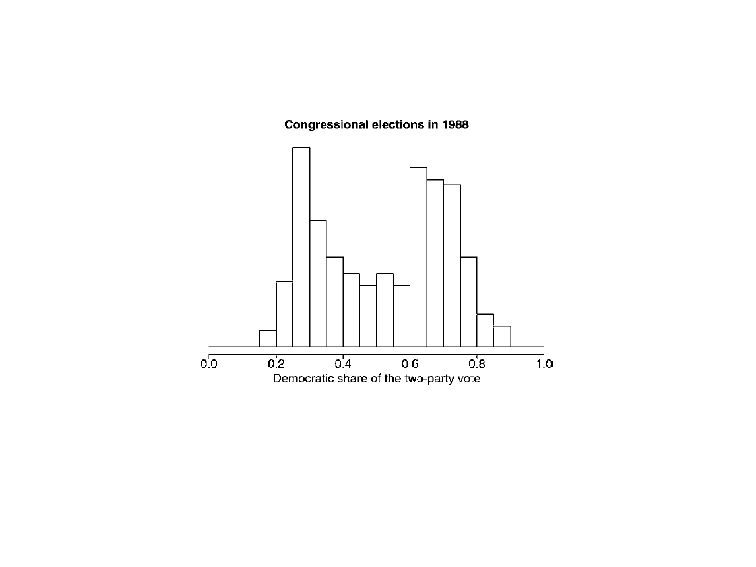
\includegraphics[width=0.5\textwidth]{img/bimodal-vote-88.pdf}
\end{center}
\begin{itemize}
\item
Histogram of Democratic share of the two-party vote in congressional
elections in 1988.
\\[8pt]
{\footnotesize Only districts contested by boty major parties shown.}
\end{itemize}

\sld{Mixture Components}
\begin{center}
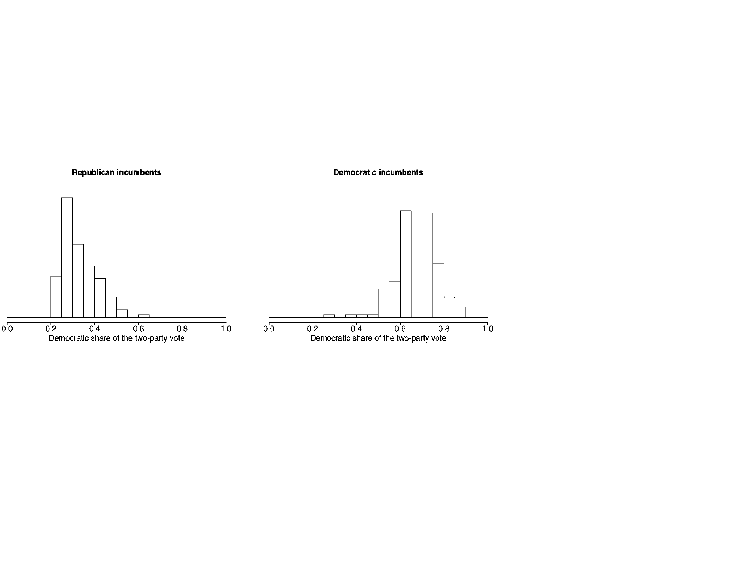
\includegraphics[width=0.85\textwidth]{img/bimodal-rep-dem.pdf}
\end{center}
\begin{itemize}
\item Incumbent in district: (left) Republican; (right) Democratic
\end{itemize}

\sld{And One More}
\begin{center}
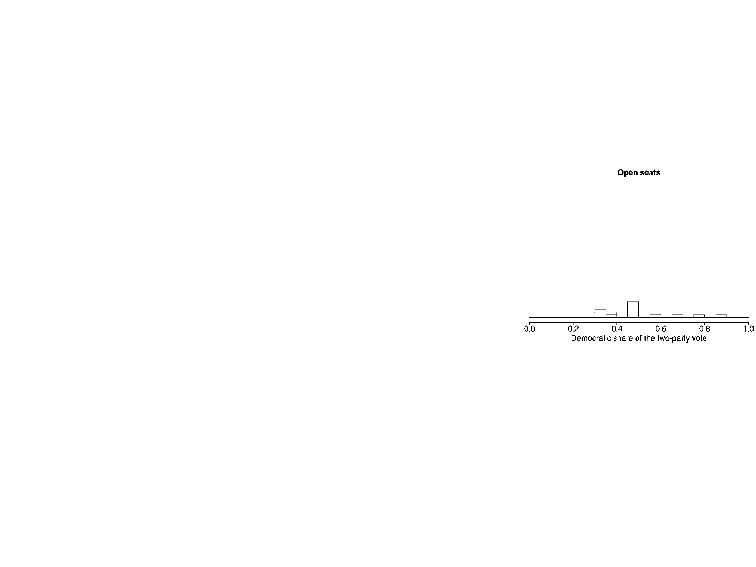
\includegraphics[width=0.3\textwidth]{img/bimodal-indy.pdf}
\end{center}
\begin{itemize}
\item Open seats
\item All three together produce a bimodal distribution
\item Number of modes is tricky to assess
\end{itemize}

\sld{Mixture of Two Normals}
\begin{itemize}
\item Assume obs.\ $y_n$ generated by one of two distributions
\begin{subitemize}
\item with some mixing proportion
\item e.g., adult height mixture of male and
  female distributions
\end{subitemize}
\item Assume i.i.d. observations
\begin{subitemize}
\item $z_n \sim \distro{Bernoulli}(\lambda)$  \hfill
    (``responsibility'' for $y_n$)
\item $y_n \sim \distro{Normal}(\mu_{z[n]}, \ \sigma_{z[n]})$
\end{subitemize}
\item Assume independent priors
\begin{subsubitemize}
\item $\lambda \sim \ldots$ \hfill $\sigma \sim \ldots$ \hfill $\mu
  \sim \ldots$ \hfill \mbox{ }
\end{subsubitemize}
\item Natural generalization to $K$ mixture components
\end{itemize}

\sld{Mixture Likelihood}
\begin{itemize}
\item Joint likelihood and responsibility
{\small
\[
\begin{array}{l}
p(y,z|\lambda,\mu,\sigma) 
\\[6pt]
\mbox{ } \ \ = \ \prod_{n=1}^N \left( 
                 \distro{Bernoulli}(z_n \, | \, \lambda) 
                 \times \distro{Normal}(y_n \, | \, \mu_{z_n}, \, \sigma_{z_n})
               \right)
\end{array}
\]
}
\item Likelihood marginalizes out responsibility
\begin{subitemize}
\item use law of total probability
\item rough notation: $p(a) = p(a,b=1) + p(a,b=0)$
\end{subitemize}
{\small
\[
\begin{array}{l}
p(y_n \, | \mu, \sigma, \lambda) 
\\[6pt]
\mbox{ } \ \ = \ \distro{Bern}(1|\lambda) \times \distro{Normal}(y|\mu_1, \sigma_1)
\\[4pt]
\mbox{ } \ \ \ \ \ \ \ \ + \ \distro{Bern}(0|\lambda) \times \distro{Normal}(y|\mu_2, \sigma_2)
\\[10pt]
\mbox{ } \ \ = \ \lambda \times \distro{Normal}(y|\mu_1, \sigma_1)
\ + \ (1 - \lambda) \times \distro{Normal}(y|\mu_2, \sigma_2)
\end{array}
\]
}
\end{itemize}

\sld{Prereq: {\Large \code{\bfseries increment\_log\_prob}}}
\begin{itemize}
\item Increment log density with expression \code{lp}
\begin{subitemize}
\item \Verb|increment_log_prob(lp);|
\end{subitemize} 
\item Following two statement same modulo constants
\begin{subitemize}
\item \Verb|y ~ normal(mu, sigma);|
\vspace*{4pt}
\item \Verb|increment_log_prob(normal_log(y, mu, sigma));| \hfill
\end{subitemize}
\item Sampling notation drops constant terms 
\begin{subitemize}
\item i.e., those depending only on data (not parameters)
\item constants not necessary for sampling or optimization
\end{subitemize}
\end{itemize}

\sld{Prereq: {\Large \code{\bfseries log\_sum\_exp}}}
\begin{itemize}
\item Goal is stable evaluation of log mixture
\begin{subitemize}
\item i.e., $\log (\alpha_1 + \alpha_2)$
\item work on log scale to prvent underflow or overflow, so
\item $\beta_k = \log \alpha_k$
\item  
$\log (\alpha_1 + \alpha_2) 
\begin{array}[t]{l} 
  \mbox{} = \ \log (\exp(\beta_1) + \exp(\beta_2))
  \\[4pt]
  \mbox{} = \ \gamma 
            + \log (\exp(\beta_1 - \gamma) + \exp(\beta_2 - \gamma))
\end{array}
$
\end{subitemize}
\item Following two expressions equal:
\begin{subitemize}
\item \Verb|log_sum_exp(lp1,lp2)|
\vspace*{3pt}
\item \Verb|log(exp(lp1) + exp(lp2))|
\end{subitemize}
\item First is more efficient and won't underflow or overflow
\end{itemize}

\sld{Mixture of Two Normals}
{\footnotesize
\begin{Verbatim}
        for (n in 1:N) {
          real lp1;  real lp2;

          lp1 <- bernoulli_log(0, lambda)               
                   + normal_log(y[n], mu[1], sigma[1]); 

          lp2 <- bernoulli_log(1, lambda)
                   + normal_log(y[n], mu[2], sigma[2]);

          increment_log_prob(log_sum_exp(lp1,lp2));  
\end{Verbatim}
}
\vspace*{2pt}
\begin{subitemize}
\item local variables reassigned
\item directly increments log posterior
\item $\mbox{log\_sum\_exp}(\alpha,\beta) = \log (\exp(\alpha) + \exp(\beta))$
\vspace*{10pt}
\end{subitemize}

\sld{Other Mixture Applications}
\begin{itemize}
\item Other multimodal data
\item Zero-inflated Poisson or hurdle models
\item Model comparison or mixture
\item Discrete change-point model
\item Hidden Markov model, Kalman filter
\item Basically, anything with latent discrete parameters, \ldots
\hfill
\item \ldots other than ones that blow up
\begin{subitemize}
\item combinatorial (e.g., regression predictor selection)
\item unbounded (e.g., Poisson model of count data)
\end{subitemize}
\end{itemize}

\sld{Hierarchical Random Effects}
\begin{itemize}
\item End with something more like what we really fit
\item Items nested in groups of similar, but differing behavior
  (e.g., purchases at different store branches)
\item Random effects logistic regression 
\begin{subitemize}
\item assumes varying intercept and slope by group
\end{subitemize}
\item (Multivariate) hiearchical prior on regression coefficients
\item Can nest hierarchies (students in classrooms in schools in
  districts)
\item Using non-nested groups creates a multilevel model
\end{itemize}

\sld{Red-State, Blue-State (simplified)}
\begin{itemize}
\item $y_n \in \setcomp{0,1}$ indicates (reported) vote
  (Rep/Dem) for voter $n$
\item $x_n \in (0,\infty)$ denotes income for voter $n$
\item $z_n \in 1{:}50$ indicates group for voter $n$
\item Logistic regression: intercept $\alpha_k$, slope $\beta_k$ vary by state
\item Likelihood
\begin{subitemize}
\item 
{\normalsize
$y_n 
\sim \distro{Bernoulli}(\mbox{logit}^{-1}(
                          \alpha_{z[n]} + \beta_{z[n]} x_n))$
}
\end{subitemize}
\item Hierarchical prior:
\begin{subitemize}
\item $\normalsize (\alpha_k, \beta_k) \sim \distro{MultiNormal}(\eta, \Sigma)$
\item hyperpriors: $\eta \sim \cdots$; \ \ \ $\Sigma \sim \cdots$ 
\end{subitemize}
\end{itemize}

\sld{Priors on Covariance Matrices}
\begin{itemize}
\item Decompose into prior on correlation matrix $\Omega$ and scale $\tau$
\item $\tau \sim \distro{Cauchy}(0, 2.5)$
\item $\Omega \sim \distro{LKJCorr}(4)$
\item $\distro{LKJCorr}(\Omega \, | \nu) \propto
  \mbox{det}(\Omega)^{\nu - 1}$
\begin{subitemize}
\item $\nu = 1$ uniform; $\nu > 1$ concentrates around unit matrix
\\ (i.e., less correlation has higher prior density)
\end{subitemize}
\item Then scale $\Omega$ by $\tau$ 
\[
\Sigma = \mbox{diag}(\tau) \, \Omega \, \mbox{diag}(\tau)
\]
where $\mbox{diag}(\tau)$ is a diagonal matrix with diagoal $\tau$
\end{itemize}

\sld{Cholesky-based Parmaterization}
\begin{itemize}
\item Parameterize more efficiently in terms of Cholesky factors
\[
\Omega = L_{\Omega} \, L_{\Omega}^{\top}
\]
\item And then take the prior to be 
\[
L_{\Omega} \sim \distro{LKJCorrCholesky}(4)
\]
and reconstruct Cholesky factor of covariance matrix by scaling
\[
L_{\Sigma} = \mbox{diag}(\tau) \, L_{\Omega}
\]
\end{itemize}

\sld{LKJ Density and Cholesky Factors}
\begin{itemize}
\item Density on \emph{correlation} \ matrices $\Omega$
%
\item $\distro{LKJCorr}(\Omega \, | \, \nu) 
       \propto \mbox{det}(\Omega)^{(\nu - 1)}$
\begin{subitemize}
\item $\nu = 1$ uniform
\item $\nu > 1$ concentrates around unit matrix
\end{subitemize}
%
\item Work with Cholesky factor $L_{\Omega}$ s.t. $\Omega = L_{\Omega} \, L_{\Omega}^{\top}$
\begin{subitemize}
\item Density: $\distro{LKJCorrCholesky}(L_{\Omega} \, | \, \nu)
\propto |J| \, \mbox{det}(L_{\Omega} \, L_{\Omega}^{\top})^{(\nu - 1)}$ 
\item Jacobian adjustment for Cholesky factorization
\end{subitemize}
%
\end{itemize}
\vfill
\hfill {\footnotesize Lewandowski, Kurowicka, and Joe (2009)}

\sld{Random Effects Priors in Stan}
\vspace*{-4pt}
{\footnotesize
\begin{Verbatim}
    parameters {
      vector[2] beta[G];  
      cholesky_factor_corr[2] L_Omega;
      vector<lower=0>[2] sigma;

    model {
      sigma ~ cauchy(0, 2.5);
      L_Omega ~ lkj_cholesky(4);
      beta ~ multi_normal_cholesky(rep_vector(0, 2),
                             diag_pre_multiply(sigma, L_Omega));
      for (n in 1:N)
        y[n] ~ bernoulli_logit(alpha[gg[n]] + x[n] * beta[gg[n]]);
\end{Verbatim}
}
\vspace*{6pt}
\begin{subitemize}
\item \code{gg[n]} indicates group for item \code{n}
\end{subitemize}


\sld{Dynamic Systems with Diff Eqs}

\begin{itemize}
\item Simple harmonic oscillator
{\small
\begin{equation*}
\frac{d}{dt} y_1 = -y_2 
\hspace*{0.5in}
\frac{d}{dt} y_2 = -y_1 - \theta y_2
\end{equation*}
}
\item Code as a function in Stan
\end{itemize}
{\footnotesize
\begin{Verbatim}
        functions {
          real[] sho(real t, real[] y, real[] theta,
                     real[] x_r, int[] x_i) {
            real dydt[2];
            dydt[1] <- y[2];
            dydt[2] <- -y[1] - theta[1] * y[2];
            return dydt;
          }
        }
\end{Verbatim}
}

\sld{Fit Noisy State Measurements}

{\footnotesize
\begin{Verbatim}
    data {
      int<lower=1> T;      real y[T,2];
      real t0;             real ts[T];
    }
    parameters {
      real y0[2];                // unknown initial state
      real theta[1];             // rates for equation
      vector<lower=0>[2] sigma;  // measurement error
    }
    model {
      real y_hat[T,2];
      ...priors...
      y_hat <- integrate_ode(sho, y0, t0, ts, theta, x_r, x_i);
      for (t in 1:T)
        y[t] ~ normal(y_hat[t], sigma);
    }
\end{Verbatim}
}

\mypart{Part II}{What Stan Does}

\sld{Full Bayes: No-U-Turn Sampler}

\begin{itemize}
\item Adaptive \myemph{Hamiltonian Monte Carlo} (HMC)
\begin{subitemize}
\item \myemph{Potential Energy}: negative log posterior
\item \myemph{Kinetic Energy}: random standard normal per iteration
\end{subitemize}
  % 
\item Adaptation \myemph{during warmup}
  \vspace*{-4pt}
  \begin{itemize}\small
  \item step size adapted to target total acceptance rate
  \item mass matrix estimated with regularization
  \end{itemize}
  % 
\item Adaptation \myemph{during sampling}
  \begin{subitemize}
  \item simulate forward and backward in time until U-turn
  \end{subitemize}
  % 
\item \myemph{Slice sample} along path
% \item \myemph{Initialization} user-specified or random unconstrained
\vfill
\hfill 
{\footnotesize (Hoffman and Gelman 2011, 2014)}
\end{itemize}


\sld{Posterior Inference}

\begin{itemize}
\item Generated quantities block for \myemph{inference}
  \\ {\footnotesize (predictions, decisions, and event probabilities)}
\item \myemph{Extractors} for samples in RStan and PyStan
\item Coda-like \myemph{posterior summary}
  \vspace*{-4pt}
  \begin{itemize}\small
  \item posterior mean w.\ MCMC std.\ error, std.\ dev., quantiles
  \item split-$\hat{R}$ multi-chain convergence diagnostic (Gelman/Rubin)
  \item multi-chain effective sample size estimation (FFT algorithm)
  \end{itemize}
\item Model comparison with \myemph{WAIC}
\begin{subitemize}
\item in-sample approximation to cross-validation
\end{subitemize}
\end{itemize}

\sld{Penalized MLE}

\begin{itemize}
\item Posterior \myemph{mode finding} via L-BFGS optimization
  \\ {\footnotesize (uses model gradient, efficiently approximates Hessian)}
\item \myemph{Disables Jacobians} for parameter inverse transforms
  \item  \myemph{Standard errors} on unconstrained scale
    \\
    {\footnotesize  (estimated using curvature of penalized log likelihood function}
\item Models, data, initialization as in MCMC
  \vfill
\item \myemph{Very Near Future}
  \vspace*{-4pt}
  \begin{itemize}\small
  \item Standard errors \myemph{on constrained scale}
    \\
    {\footnotesize  (sample unconstrained approximation and inverse transform)}
  \end{itemize}      
\end{itemize}

\sld{``Black Box'' Variational Inference}
\begin{itemize}
%
\item \myemph{Black box} so can fit any Stan model
%
\item Multivariate \myemph{normal approx to unconstrained} posterior
\begin{subitemize}
\item covariance: diagonal mean-field or full rank
\item not Laplace approx --- around posterior mean, not mode
\item transformed back to constrained space (built-in Jacobians)
\end{subitemize}
%
\item Stochastic \myemph{gradient-descent} optimization
\begin{subitemize}
\item ELBO gradient estimated via Monte Carlo + autdiff
\end{subitemize}
%
\item Returns \myemph{approximate posterior} mean / covariance
\item Returns \myemph{sample} transformed to constrained space
\end{itemize}


\sld{Stan as a Research Tool}

\begin{itemize}
\item Stan can be used to \myemph{explore algorithms}
\item Models transformed to \myemph{unconstrained support} on $\mathbb{R}^n$
\item Once a model is compiled, have
  \vspace*{-4pt}
  \begin{itemize}\small
  \item \myemph{log probability, gradient, and Hessian}
  \item data I/O and parameter initialization
  \item model provides variable names and dimensionalities
  \item transforms to and from constrained representation 
    \\ {\footnotesize (with or without Jacobian)}
  \end{itemize}
\end{itemize}


\mypart{Part III}{How Stan Works}

\sld{Model: Read and Transform Data}
\begin{itemize}
\item Only done once for optimization or sampling (per chain)
\item Read data
\begin{subitemize}
\item read data variables from memory or file stream
\item validate data
\end{subitemize}
\item Generate transformed data
\begin{subitemize}
\item execute transformed data statements
\item validate variable constraints when done
\end{subitemize}
\end{itemize}

\sld{Model: Log Density}
\begin{itemize}
\item \emph{Given} parameter values on unconstrained scale
\item Builds expression graph for log density (start at 0)
\item Inverse transform parameters to constrained scale
\begin{subitemize}
\item constraints involve non-linear transforms
\item e.g.,  positive constrained $x$ to unconstrained $y = \log x$
\end{subitemize}
\item account for curvature in change of variables
\begin{subitemize}
\item e.g., unconstrained $y$ to positive $x = \log^{-1}(y) =
  \exp(y)$
\item e.g., add log Jacobian determinant, $\log |\frac{d}{dy} \exp(y)| = y$
\end{subitemize}
\item Execute model block statements to increment log density
\end{itemize}

\sld{Model: Log Density Gradient}
\begin{itemize}
\item Log density evaluation builds up expression graph
\begin{subitemize}
\item templated overloads of functions and operators
\item efficient arena-based memory management
\end{subitemize}
\item Compute gradient in backward pass on expression graph 
\begin{subitemize}
\item propagate partial derivatives via chain rule
\item work backwards from final log density to parameters
\item dynamic programming for shared subexpressions
\end{subitemize}
\item Linear multiple of time to evalue log density
\end{itemize}

\sld{Model: Generated Quantities}
\begin{itemize}
\item \myemph{Given} parameter values
\item Once per iteration (not once per leapfrog step)
\item May involve (pseudo) random-number generation
\begin{subitemize}
\item Executed generated quantity statements
\item Validate values satisfy constraints
\end{subitemize}
\item Typically used for 
\begin{subitemize}
\item Event probability estimation
\item Predictive posterior estimation
\end{subitemize}
\item Efficient because evaluated with \code{double} types (no autodiff)
\end{itemize}

\sld{Optimize: \ L-BFGS}
\begin{itemize}
\item Initialize unconstrained parameers
\begin{subitemize}
\item Random values on unconstrained scale uniform in $(-2,2)$
\item User specified on constrained scale, transformed
\end{subitemize}
\item While not converged
\begin{subitemize}
\item Move unconstrained parameters toward optimum based on Hessian approximation and
  step size (Newton step)
\item If diverged (arithmetic error or out of support), reduce step size, continue
\item else if converged (parameter change, log density change, gradient
  value), return value
\item else update Hessian approx. based on calculated gradient
\end{subitemize}
\end{itemize}

\sld{Sample: Hamiltonian Flow}
\vspace*{-4pt}
\begin{itemize}
\item Generate random \myemph{kinetic energy} 
\vspace*{-2pt}
\begin{subitemize}
\item random $\distro{Normal}(0,1)$ in each parameter
\end{subitemize}
\item Use negative log posterior as \myemph{potential energy}
\item Hamiltonian is kinetic plus potential energy
\item \myemph{Leapfrog Integration}: for \emph{fixed} stepsize (time discretization), number of
  steps (total time), and mass matrix,
\begin{subitemize}
\item update momentum half-step based on potential (gradient)
\item update position full step based on momentum
\item update momentum half-step based on potential
\end{subitemize}
\footnotesize
\item Numerical solution of Hamilton's first-order version of
  Newton's second-order diff-eqs of motion ($\mbox{force} =
  \mbox{mass} \times \mbox{acceleration}$)
\end{itemize}

\sld{Sample: Leapfrog Example}
\begin{center}
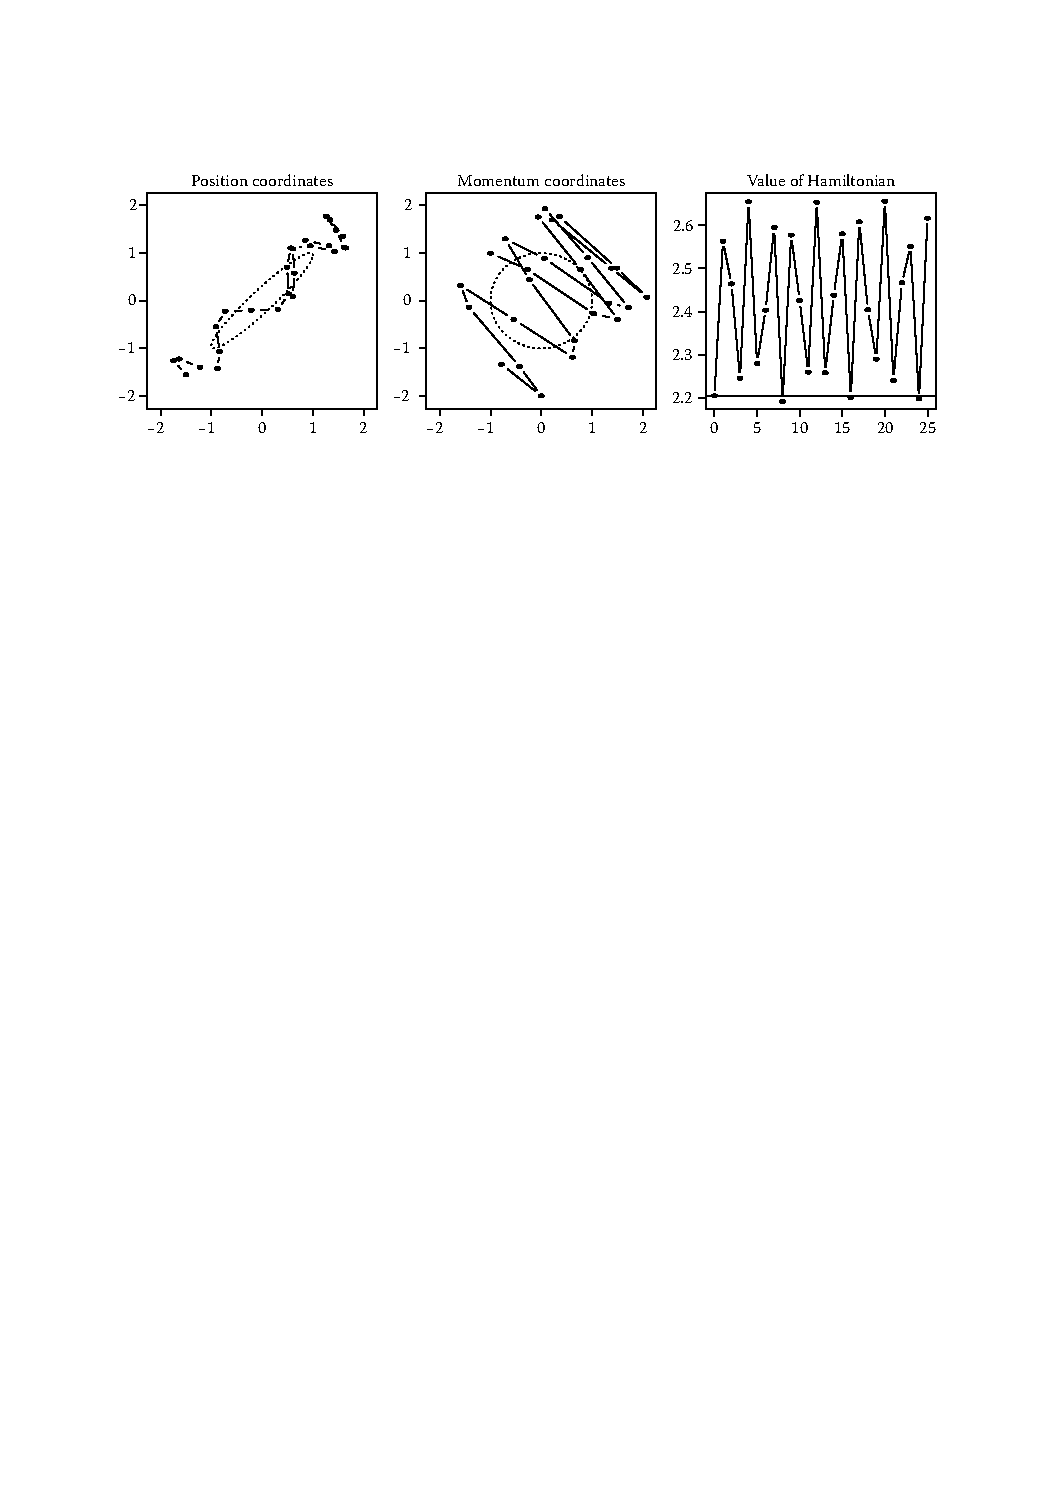
\includegraphics[width=0.9\textwidth]{img/neal-leapfrog.pdf}
\end{center}
\vspace*{-8pt}
\begin{subitemize}
\item \small Trajectory of 25 leapfrog steps for correlated 2D normal (ellipses at 1 sd
  from mean), stepsize of 0.25, initial state of $(-1,1)$, and initial
  momentum of $(-1.5,-1.55)$.  
\\[12pt]
\footnotesize Radford Neal (2013) MCMC using Hamiltonian Dynamics. In {\slshape Handbook
of MCMC}. (free online at \url{http://www.mcmchandbook.net/index.html})
\end{subitemize}


\sld{Sample: No-U-Turn Sampler (NUTS)}
\begin{itemize}
\item Adapts Hamiltonian simulation time
\begin{subitemize}
\item goal to maximize mixing, maintaining detailed balance
\item too short devolves to random walk
\item too long does extra work (i.e., orbits)
\end{subitemize}
\item For exponentially increasing number of steps up to max
\begin{subitemize}
\item Randomly choose to extend forward or backward in time
\item Move forward or backward in time number of steps
\begin{subsubitemize}
\item stop if any subtree (size 2, 4, 8, ...) makes U-turn
\item remove all current steps if subtree U-turns (not ends)
\end{subsubitemize}
\end{subitemize}
\item Randomly select param with density above slice (or reject)
\end{itemize}

\sld{Sample: NUTS Binary Tree}
\vspace*{-6pt}
\begin{center}
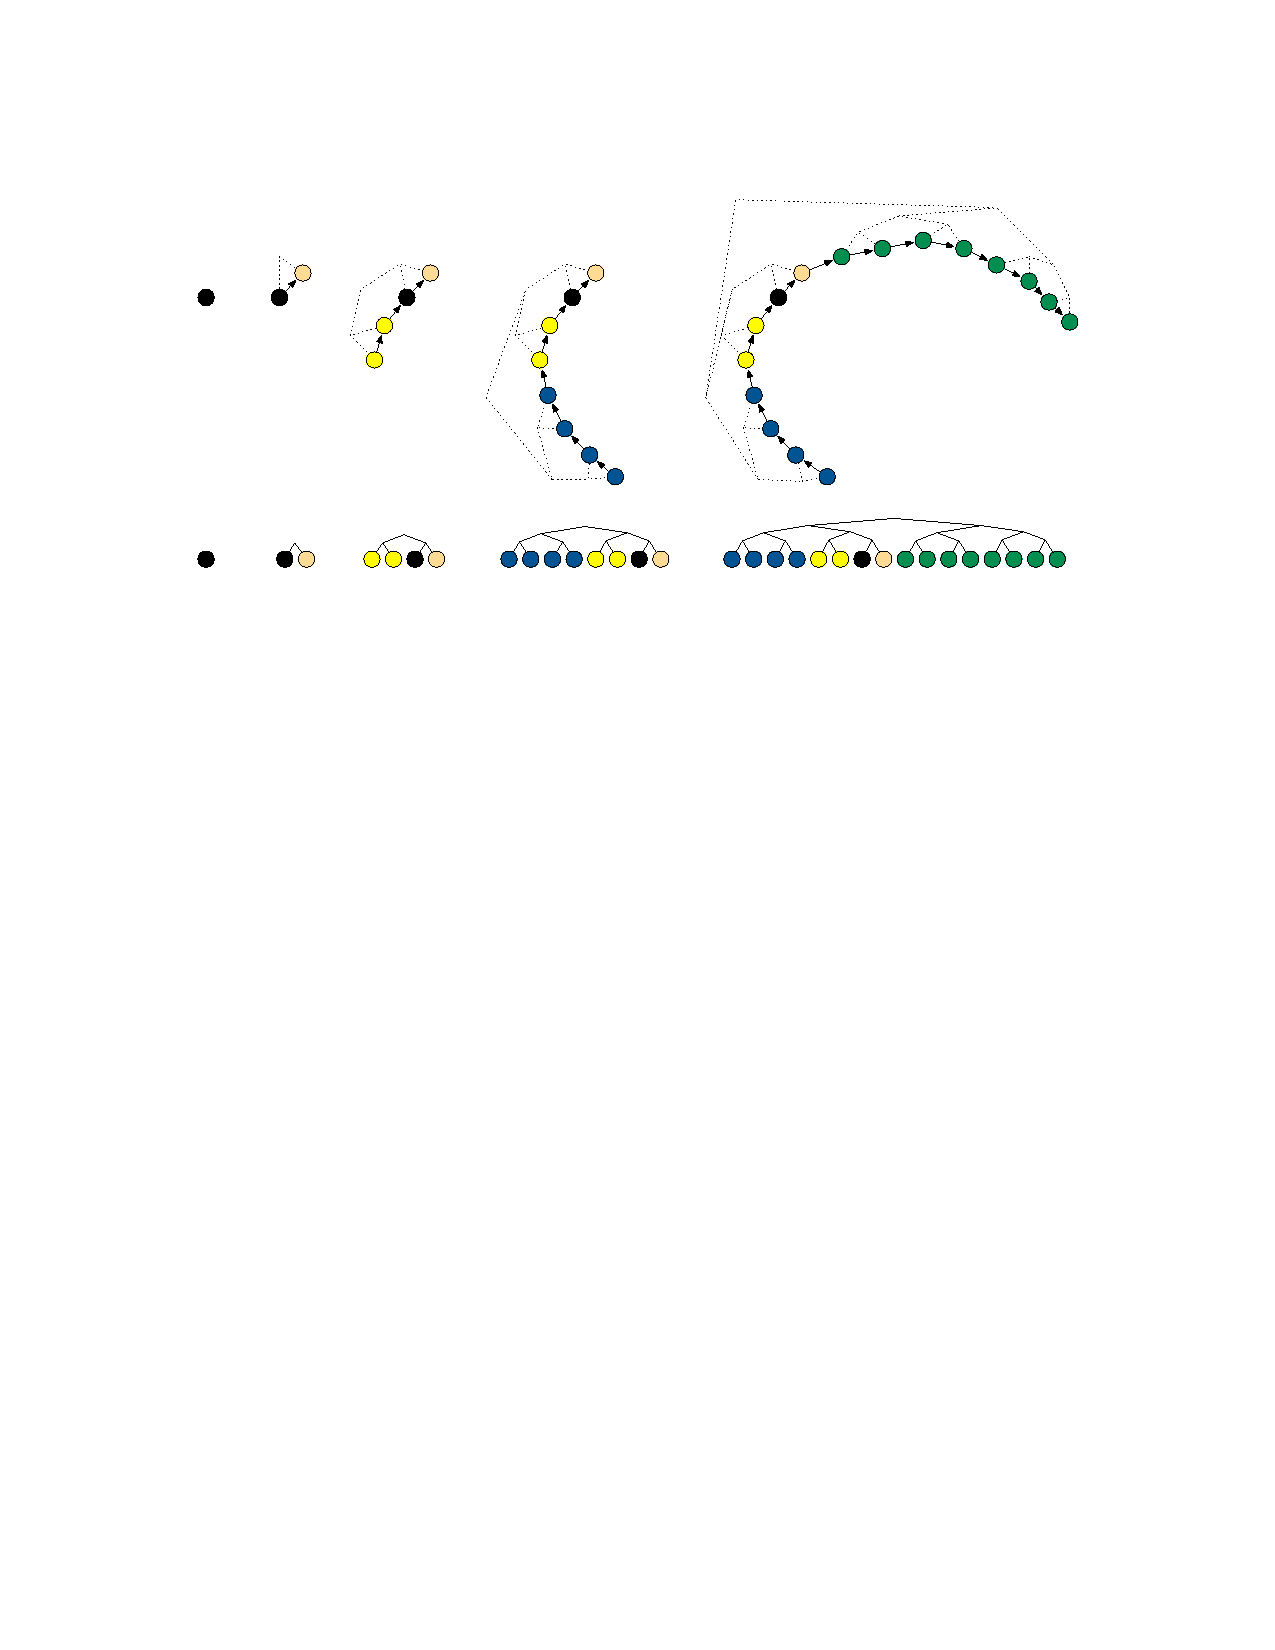
\includegraphics[width=0.9\textwidth]{img/NUTS-tree-evolution.pdf}
\end{center}
\begin{subitemize}
\item Example of repeated doubling building binary tree forward and
  backward in time until U-turn.  
\\[3pt]
\footnotesize
Hoffman and Gelman. 2014. The No-U-Turn Sampler. {\slshape JMLR}.
(free online at \url{http://jmlr.org/papers/v15/hoffman14a.html})
\end{subitemize}

\sld{Sample: NUTS U-Turn}
\\[4pt]
\hspace*{8pt}
\begin{minipage}{0.65\textwidth}
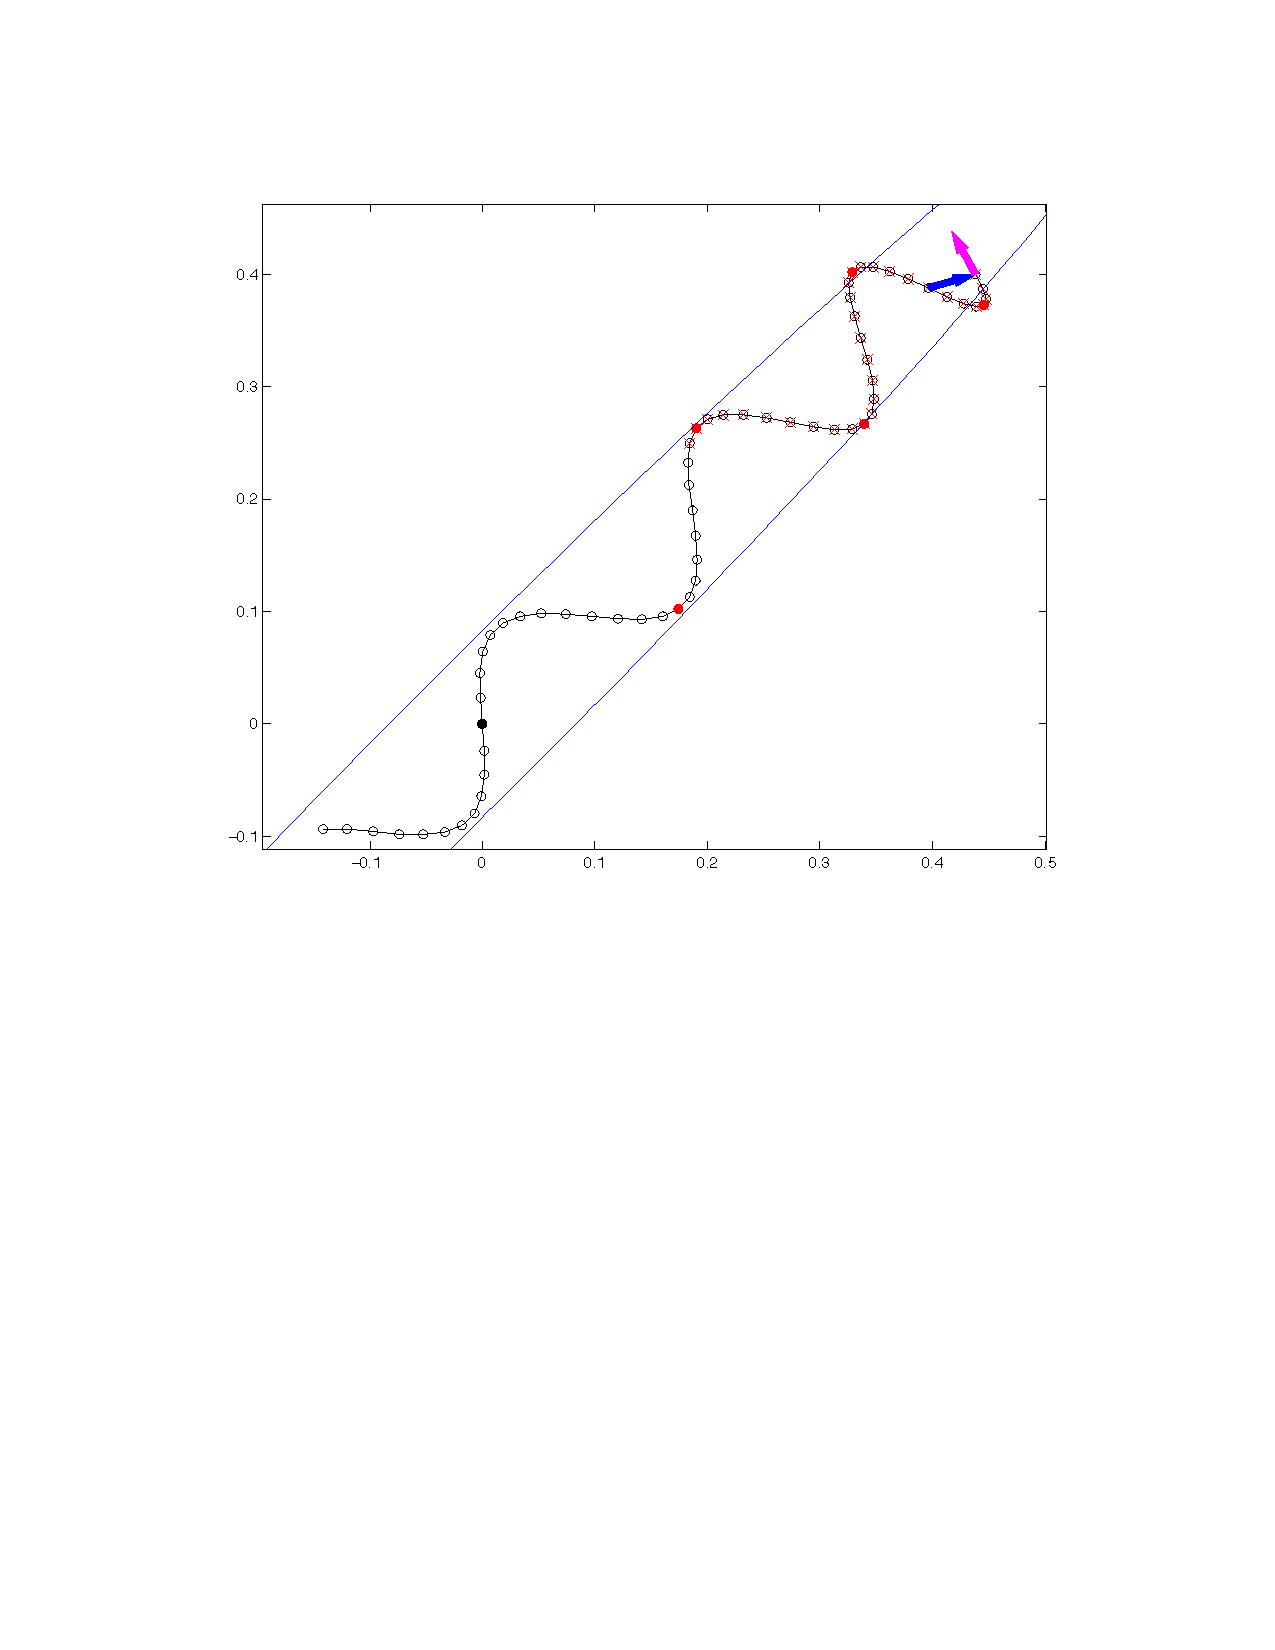
\includegraphics[width=\textwidth]{img/NUTS-trajectory.pdf}
\end{minipage}
\hspace*{-24pt}
\begin{minipage}{0.35\textwidth}
\footnotesize
\begin{subsubitemize}
\item Example of trajectory from one iteration of NUTS.
\item Blue ellipse
  is contour of 2D normal.  
\item Black circles are leapfrog steps.
\item Solid red circles excluded below slice
\item U-turn made with blue and magenta
  arrows
\item  Red crossed circles excluded for detailed balance
\end{subsubitemize}
\end{minipage}

\sld{Sample: HMC/NUTS Warmup}
\begin{itemize}
\item Estimate stepsize 
\begin{subitemize}
\item too small requires too many leapfrog steps
\item too large induces numerical inaccuracy
\item need to balance
\end{subitemize}
\item Estimate mass matrix
\begin{subitemize}
\item Diagonal accounts for parameter scales
\item Dense optionally accounts for rotation
\end{subitemize}
\end{itemize}


\sld{Sample: Warmup (cont.)}
\begin{itemize}
\item Initialize unconstrained parameters as for optimization
\item For exponentially increasing block sizes
\begin{subitemize}
\item for each iteration in block
%
\begin{subsubitemize}
\item generate random kinetic energy
\item simulate Hamiltonian flow (HMC fixed time, NUTS adapts)
\item choose next state (Metroplis for HMC, slice for NUTS)
\end{subsubitemize}
%
\item update regularized point estimate of mass matrix
\begin{subsubitemize}
\item use parameter draws from current block
\item shrink diagonal toward unit; dense toward diagonal
\end{subsubitemize}
\item tune stepsize (line search) for target acceptance rate
\end{subitemize}
\end{itemize}

\sld{Sample: HMC/NUTS Sampling}
\begin{itemize}
\item Fix stepsize and and mass matrix
\item For sampling iterations
\begin{subitemize}
\item generate random kinetic energy
\item simulate Hamiltonian flow
\item apply Metropolis accept/reject (HMC) or slice (NUTS)
\end{subitemize}
\end{itemize}

\sld{NUTS vs.\ Gibbs and Metropolis}

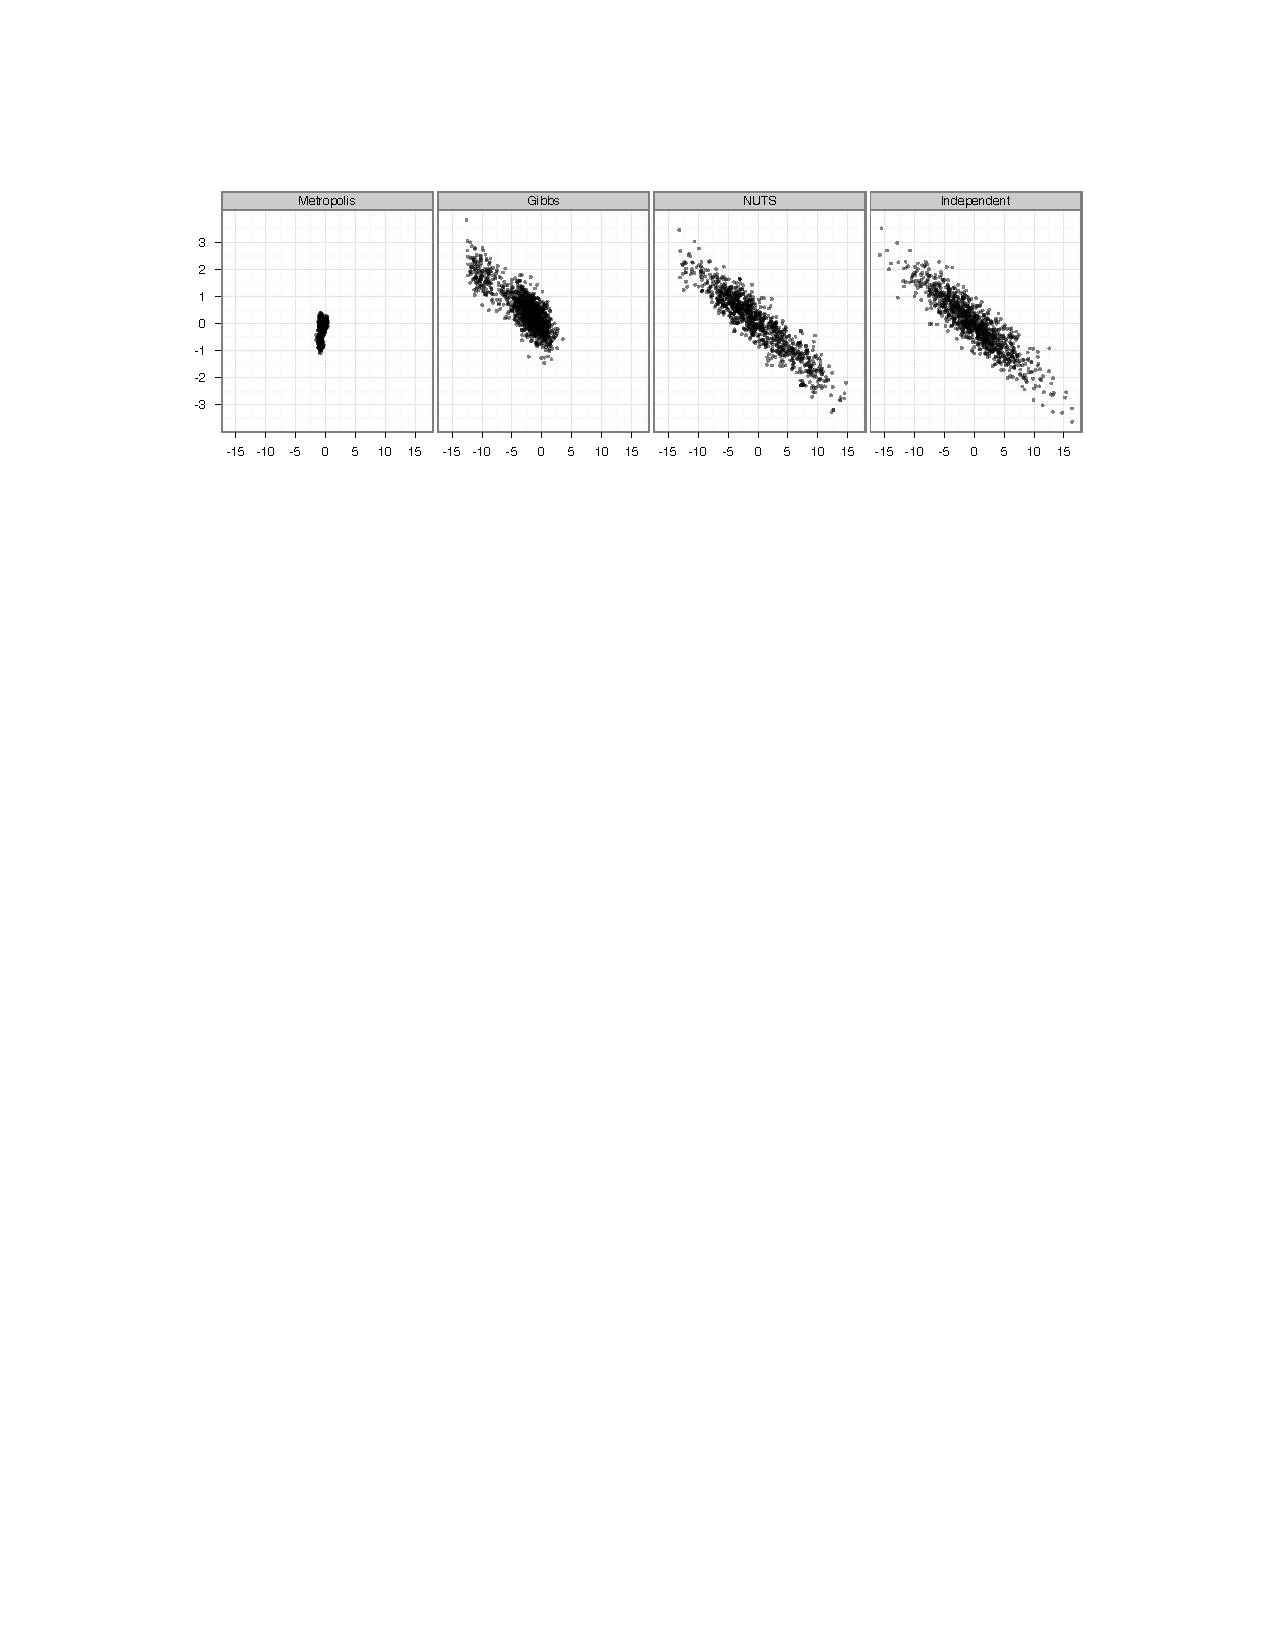
\includegraphics[width=0.9\textwidth]{img/nuts-vs.pdf}
\begin{subitemize}
\item Two dimensions of highly correlated 250-dim normal
\item \myemph{1,000,000 draws} from Metropolis and Gibbs (thin to 1000)
\item \myemph{1000 draws} from NUTS; 1000 independent draws
\end{subitemize}

\sld{NUTS vs.\ Basic HMC}

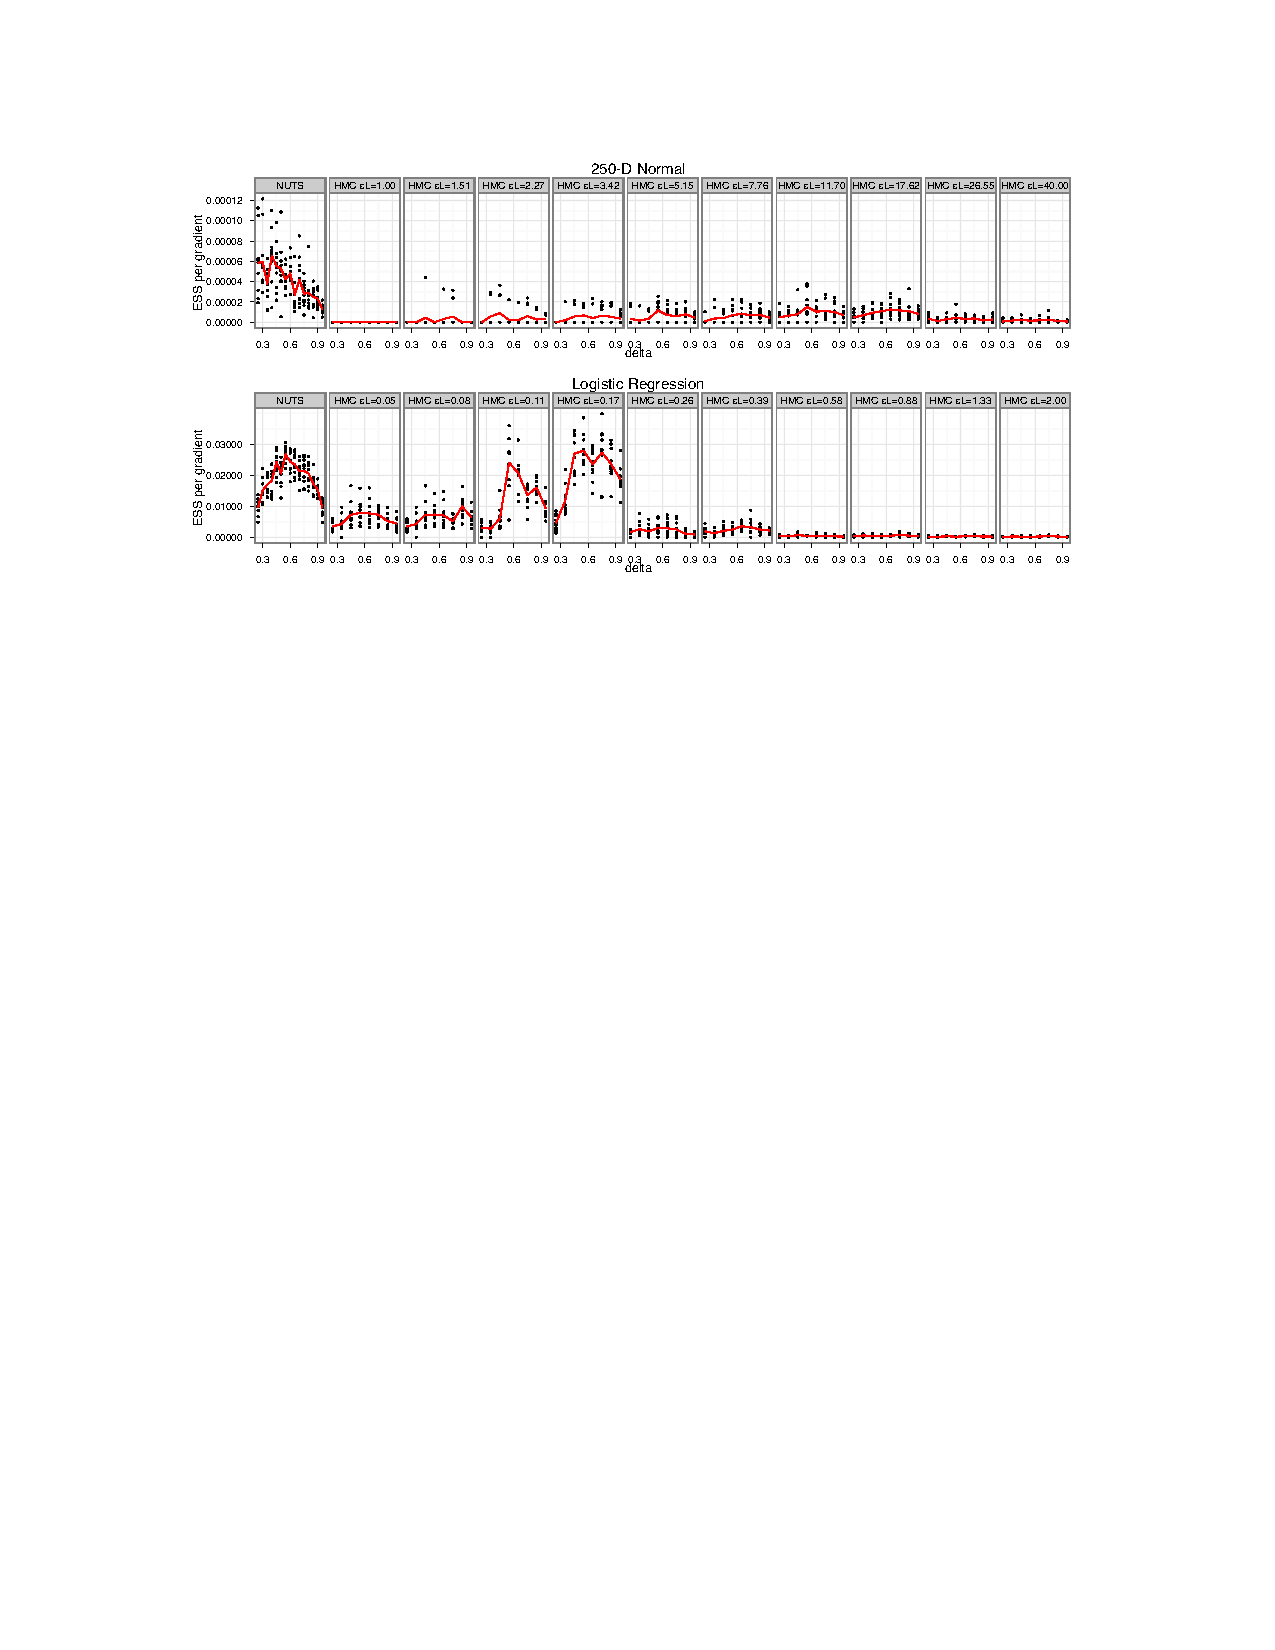
\includegraphics[width=0.9\textwidth]{img/nuts-ess-1.pdf}
{\small
  \begin{itemize}
  \item 250-D normal and logistic regression models
  \item Vertical axis is effective sample size per sample (bigger better)
  \item Left) NUTS; \ \ Right) HMC with increasing $t = \epsilon L$
  \end{itemize}
}

\sld{NUTS vs.\ Basic HMC II}

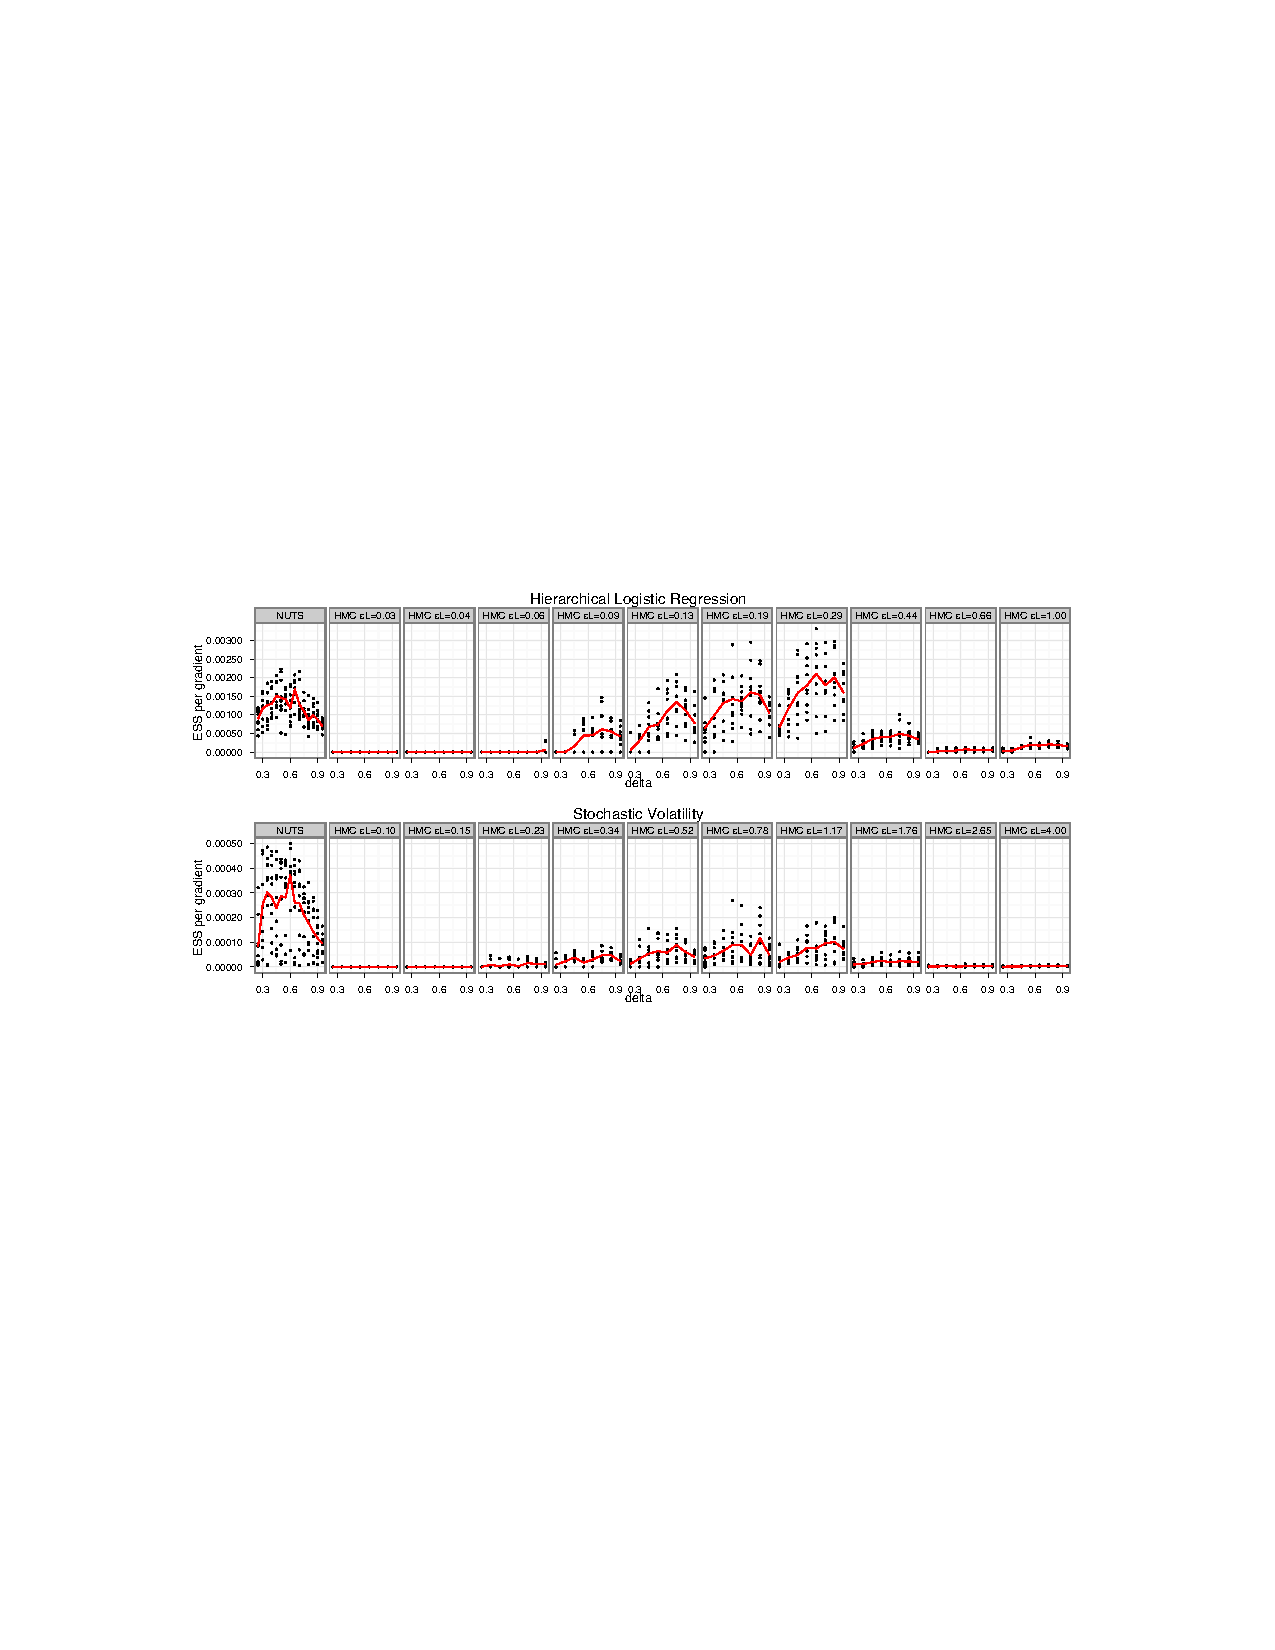
\includegraphics[width=0.9\textwidth]{img/nuts-ess-2.pdf}

{\small
  \begin{itemize}
  \item Hierarchical logistic regression and stochastic volatility
  \item Simulation time $t$ is $\epsilon \ L$, step size ($\epsilon$)
    times number of steps ($L$)
  \item NUTS can beat optimally tuned HMC (latter very expensive)
  \end{itemize}
}



\mypart{Part IV}{Stan Language}

\sld{Basic Program Blocks}

\begin{itemize}
\item \myemph{\tt\bfseries data} \ (once) 
  \vspace*{-4pt}
  \begin{itemize}\small
  \item {\slshape content}: declare data types, sizes, and constraints
  \item {\slshape execute}: read from data source, validate constraints
  \end{itemize}
  % 
\item \myemph{\tt\bfseries parameters} \ (every log prob eval)
  \vspace*{-4pt}
  \begin{itemize}\small
  \item {\slshape content}: declare parameter types, sizes, and constraints
  \item {\slshape execute}: transform to constrained, Jacobian
  \end{itemize}
  % 
\item \myemph{\tt\bfseries model} \ (every log prob eval) 
  \vspace*{-4pt}
  \begin{itemize}\small
  \item {\slshape content}: statements definining posterior density
  \item {\slshape execute}: execute statements
  \end{itemize}
\end{itemize}

\sld{Derived Variable Blocks}

\begin{itemize}
\item \myemph{\tt\bfseries transformed data} (once after data)
  \vspace*{-4pt}
  \begin{itemize}\small
  \item {\slshape content}: declare and define transformed data variables
  \item {\slshape execute}: execute definition statements, validate constraints
  \end{itemize}
  % 
\item \myemph{\tt\bfseries transformed parameters} (every log prob eval)
  \vspace*{-4pt}
  \begin{itemize}\small
  \item {\slshape content}: declare and define transformed parameter vars
  \item {\slshape execute}: execute definition statements, validate constraints
  \end{itemize}
  % 
\item \myemph{\tt\bfseries generated quantities} (once per draw, 
  \code{double} type)
  \vspace*{-4pt}
  \begin{itemize}\small
  \item {\slshape content}: declare and define generated quantity
    variables; \\
    includes pseudo-random number generators
    \\
    {\footnotesize (for posterior predictions, event probabilities,
      decision making)}
  \item {\slshape execute}: execute definition statements, validate constraints
  \end{itemize}
  % 
\end{itemize}


\sld{Variable and Expression Types}
\\[3pt]
\hspace*{17pt}Variables and expressions are \myemph{strongly, statically typed}.
\begin{itemize}
\item \myemph{Primitive}: {\tt\small int}, \ {\tt\small real}
\item \myemph{Matrix}: {\tt\small matrix[M,N]}, \ {\tt\small vector[M]}, \ {\tt\small row\_vector[N]}
\item \myemph{Bounded}: primitive or matrix, with 
  \\ {\tt\small <lower=L>}, \ {\tt\small <upper=U>}, \ {\tt\small <lower=L,upper=U>}
\item \myemph{Constrained Vectors}: {\tt\small simplex[K]}, \ {\tt\small
    ordered[N]},
  \\ {\tt\small positive\_ordered[N]}, \ {\tt\small unit\_length[N]}
\item \myemph{Constrained Matrices}: {\tt\small cov\_matrix[K]}, \ {\tt\small
    corr\_matrix[K]}, \ {\tt\small cholesky\_factor\_cov[M,N]}, \
  {\tt\small cholesky\_factor\_corr[K]}
\item \myemph{Arrays:}  of any type (and dimensionality)
\end{itemize}

\sld{Logical Operators}
\vfill
\noindent\spc
{\footnotesize
  \begin{tabular}{c|ccl|l}
    {\it Op.} & {\it Prec.} & {\it Assoc.} & {\it
      Placement} & {\it Description}
    \\ \hline \hline
    \code{||} & 9 & left & binary infix & logical or
    \\ \hline
    \Verb|&&| & 8 & left & binary infix & logical and
    \\ \hline
    \Verb|==| & 7 & left & binary infix & equality
    \\
    \Verb|!=| & 7 & left & binary infix & inequality
    \\ \hline
    \Verb|<| & 6 & left & binary infix & less than
    \\
    \Verb|<=| & 6 & left & binary infix & less than or equal
    \\
    \Verb|>| & 6 & left & binary infix & greater than 
    \\
    \Verb|>=| & 6 & left & binary infix & greater than or equal
  \end{tabular}
}
\vfill
\vfill

\sld{Arithmetic and Matrix Operators}
\vfill
\noindent\spc
{\footnotesize
  \begin{tabular}{c|ccl|l}
    {\it Op.} & {\it Prec.} & {\it Assoc.} & {\it
      Placement} & {\it Description}
    \\ \hline \hline

    \code{+} & 5 & left & binary infix & addition
    \\
    \code{-} & 5 & left & binary infix & subtraction
    \\ \hline
    \code{*} & 4 & left & binary infix & multiplication
    \\
    \code{/} & 4 & left & binary infix & (right) division
    \\ \hline
    \Verb|\| & 3 & left & binary infix & left division
    \\ \hline
    \code{.*} & 2 & left & binary infix & elementwise multiplication
    \\
    \code{./} & 2 & left & binary infix & elementwise division
    \\ \hline
    \code{!} & 1 & n/a & unary prefix & logical negation
    \\
    \code{-} & 1 & n/a & unary prefix & negation
    \\ 
    \code{+} & 1 & n/a & unary prefix & promotion (no-op in Stan)
    \\ \hline
    \Verb|^| & 2 & right & binary infix & exponentiation
    \\ \hline
    \code{'} & 0 & n/a & unary postfix & transposition
    \\ \hline \hline
    \code{()} & 0 & n/a & prefix, wrap & function application
    \\
    \code{[]} & 0 & left & prefix, wrap & array, matrix indexing
  \end{tabular}
}
\vfill

\sld{Built-in Math Functions}

\begin{itemize}
\item All built-in \myemph{C++ functions and operators}
  \\
  {\footnotesize C math, TR1, C++11, including all trig, pow, and
    special log1m, erf, erfc, fma, atan2, etc.}
\item Extensive library of \myemph{statistical functions}
  \\
  {\footnotesize e.g., softmax,
    log gamma and digamma functions, beta functions, Bessel functions of
    first and second kind, etc.}
  % 
\item Efficient, arithmetically stable \myemph{compound functions}
  \\
  {\footnotesize e.g., multiply log, log sum of
    exponentials, log inverse logit}
\end{itemize}

\sld{Built-in Matrix Functions}

\begin{itemize}\small
\item \myemph{Basic arithmetic}: all arithmetic operators
\item \myemph{Elementwise arithmetic}: vectorized operations
\item \myemph{Solvers}: matrix division, (log) determinant,
  inverse 
\item \myemph{Decompositions}: QR, Eigenvalues and Eigenvectors, 
  \\
  Cholesky factorization, singular value decomposition
\item \myemph{Compound Operations}: quadratic forms, variance scaling, etc.
\item \myemph{Ordering, Slicing, Broadcasting}: sort, rank, block, rep
\item \myemph{Reductions}: sum, product, norms
\item \myemph{Specializations}: triangular, positive-definite,
\end{itemize}

\sld{User-Defined Functions}

\begin{itemize}
\item \myemph{\tt\bfseries functions} \ (compiled with model)
  \vspace*{-4pt}
  \begin{itemize}\small
  \item {\slshape content}: declare and define general (recursive) functions
    \\
    {\small (use them elsewhere in program)}
  \item {\slshape execute}: compile with model
  \end{itemize}
  \vspace*{6pt}
\item Example
  \\[6pt]
  \begin{minipage}[t]{0.8\textwidth}
    \footnotesize
    \begin{Verbatim}
      functions {

        real relative_difference(real u, real v) {
          return 2 * fabs(u - v) / (fabs(u) + fabs(v));
        }

      }
    \end{Verbatim}
  \end{minipage}
\end{itemize}

\sld{Differential Equation Solver}
\begin{itemize}
\item System expressed as function
\begin{subitemize}
\item given state ($y$) time ($t$), parameters ($\theta$), and data ($x$)
\item return derivatives ($\partial y / \partial t$) of state w.r.t. time
\end{subitemize}
\item Simple harmonic oscillator diff eq
{\footnotesize
\begin{Verbatim}
    real[] sho(real t,         // time
               real[] y,       // system state
               real[] theta,   // params
               real[] x_r,     // real data
               int[] x_i) {    // int data
      real dydt[2];
      dydt[1] <- y[2];
      dydt[2] <- -y[1] - theta[1] * y[2];
      return dydt;
   }
\end{Verbatim}
}
\end{itemize}

\sld{Differential Equation Solver}
\begin{itemize}
\item Solution via functional, given initial state (\code{y0}), 
initial time (\code{t0}), desired solution times (\code{ts})
{\footnotesize
\begin{Verbatim}
  mu_y <- integrate_ode(sho, y0, t0, ts, theta, x_r, x_i);
\end{Verbatim}
}
\item Use noisy measurements of $y$ to estimate $\theta$
\begin{Verbatim}
y ~ normal(mu_y, sigma);
\end{Verbatim}
\begin{subitemize}
\item Pharmacokinetics/pharmacodynamics (PK/PD),
\item soil carbon respiration with biomass input and breakdown
\end{subitemize}
\end{itemize}

\sld{Diff Eq Derivatives}
\begin{itemize}
\item Need derivatives of solution w.r.t.\ parameters
\item Couple derivatives of system  w.r.t. parameters
\[
\left( 
\frac{\partial}{\partial t} \, y, \ \
\frac{\partial}{\partial t} \, \frac{\partial y}{\partial \theta}
\right)
\]
\item Calculate coupled system via nested autodiff of second term
\[
\frac{\partial}{\partial \theta}
\,
\frac{\partial y}{\partial t}
\]
\end{itemize}

\sld{Distribution Library}

\begin{itemize}
\item Each distribution has
  \vspace*{-4pt}
  \begin{itemize}\small
  \item log density or mass function
  \item cumulative distribution functions, plus complementary versions,
    plus log scale
  \item Pseudo-random number generators
  \end{itemize}
\item Alternative parameterizations
  \\
  {\footnotesize (e.g., Cholesky-based multi-normal,
    log-scale Poisson, logit-scale Bernoulli)}
\item New multivariate correlation matrix density: LKJ
  \\
  {\footnotesize degrees of freedom controls 
    shrinkage to (expansion from) unit matrix}
\end{itemize}

\sld{Statements}
\vspace*{-4pt}
\begin{itemize}
\item \myemph{Sampling}: \ {\footnotesize \Verb|y ~ normal(mu,sigma)|}
  \ \ \ {\footnotesize (increments log probability)}
  % 
\item \myemph{Log probability}: \ {\footnotesize increment\_log\_prob(lp);}
\item \myemph{Assignment}: \  {\footnotesize \code{y\_hat <- x * beta};}
  % 
\item \myemph{For loop}: \ {\footnotesize \code{for (n in 1:N) ...}}
  % 
\item \myemph{While loop}: \ {\footnotesize \code{while (cond) ...}}
  % 
\item \myemph{Conditional}: \ {\footnotesize
    \code{if (cond) ...; else if (cond) ...;  else ...;}}
\item \myemph{Block}: \ {\footnotesize \Verb|{ ... }|}  \ \ \ {\footnotesize
    (allows local variables)}
\item \myemph{Print}: \ {\footnotesize \code{print("theta=",theta);}}
\item \myemph{Reject}: 
\ {\footnotesize 
    \code{reject("arg to foo must be positive, found y=", y);}}
\end{itemize}


\mypart{Part V}{Challenges for Stan}

\sld{Models with Discrete Parameters}
\begin{itemize}
\item e.g., simple mixture models, survival models, HMMs,
  discrete measurement error models, missing data
\item \myemph{Marginalize out} discrete parameters
\item Efficient sampling due to \myemph{Rao-Blackwellization}
\item Inference straightforward with expectations
  \vspace*{12pt}
\item Probability-programming combo too \myemph{difficult} for many of our target users
  \\
  {\small (exploring encapsulation options)}
\end{itemize}

\sld{Models with Missing Data}
\begin{itemize}
\item In principle, missing data just \myemph{additional parameters}
\item In practice, how to declare? 
  \begin{itemize}
  \item \myemph{observed} data as data variables
  \item \myemph{missing} data as parameters
  \item combine into single vector 
    \\ {\footnotesize (in transformed parameters or local in model)}
  \end{itemize}
\end{itemize}

\sld{Global Mass Matrix Adaptation}
\vspace*{-4pt}
\begin{itemize}
\item Mass matrix provides \myemph{global} adaptation for
\begin{subitemize}
\item parameter scale (diagonal)
\item rotation (dense)
\end{subitemize}
%
\item Scaling necessary, but breaks rotation invariance of HMC
%
\item Dense mass matrices (rotation) challenging to estimate
\begin{subitemize}
\item $\bigoh{N^2}$ estimands
\item dimensionality defeats exploring all directions
\item chicken-and-egg problem
\item hard to regularize point estimates
\item why adaptive Metropolis-Hastings so difficult
\end{subitemize}
\end{itemize}

\sld{Position-Dependent Curvature}
\begin{itemize}
\item \myemph{Problem}: Position-dependent curvature
\begin{subitemize}
\item Example: banana-shaped densities
\begin{subsubitemize}
\item arise when parameter is product of other parameters
\end{subsubitemize}
\item Example: hierarchical models
\begin{subsubitemize}
\item hierarhcical variance controls lower-level parameters
\end{subsubitemize}
\end{subitemize}
\item Mitigate problem by reducing step size
\begin{subsubitemize}
\item Stan: initial (\code{stepsize}) and target acceptance (\code{adapt\_delta})
\end{subsubitemize}
\end{itemize}


\sld{Hierarchical Model: Funnel}
\vspace*{-8pt}
\[
p(y,x) = \distro{Normal}(y \, | \, 0,3) \times \prod_{n=1}^9
\distro{Normal}(x_n \, | \, 0,\ \exp(y/2)).
\]
\begin{center}
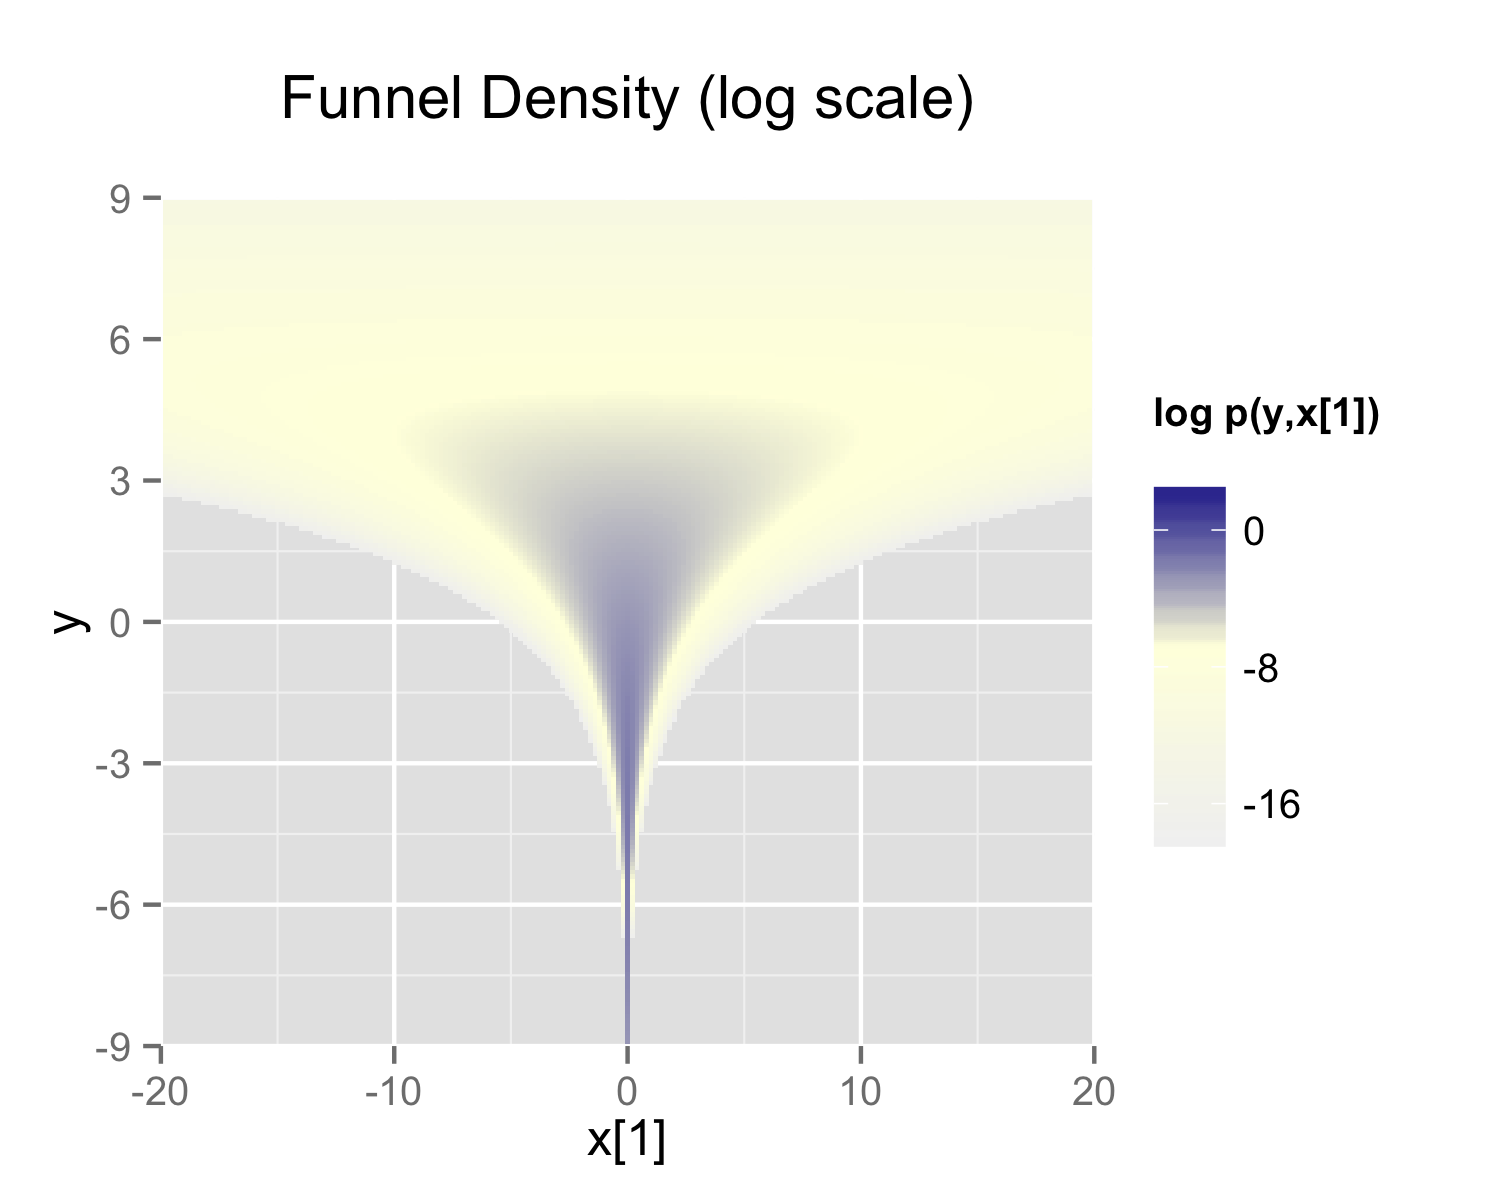
\includegraphics[width=0.52\textwidth]{img/funnel.png}
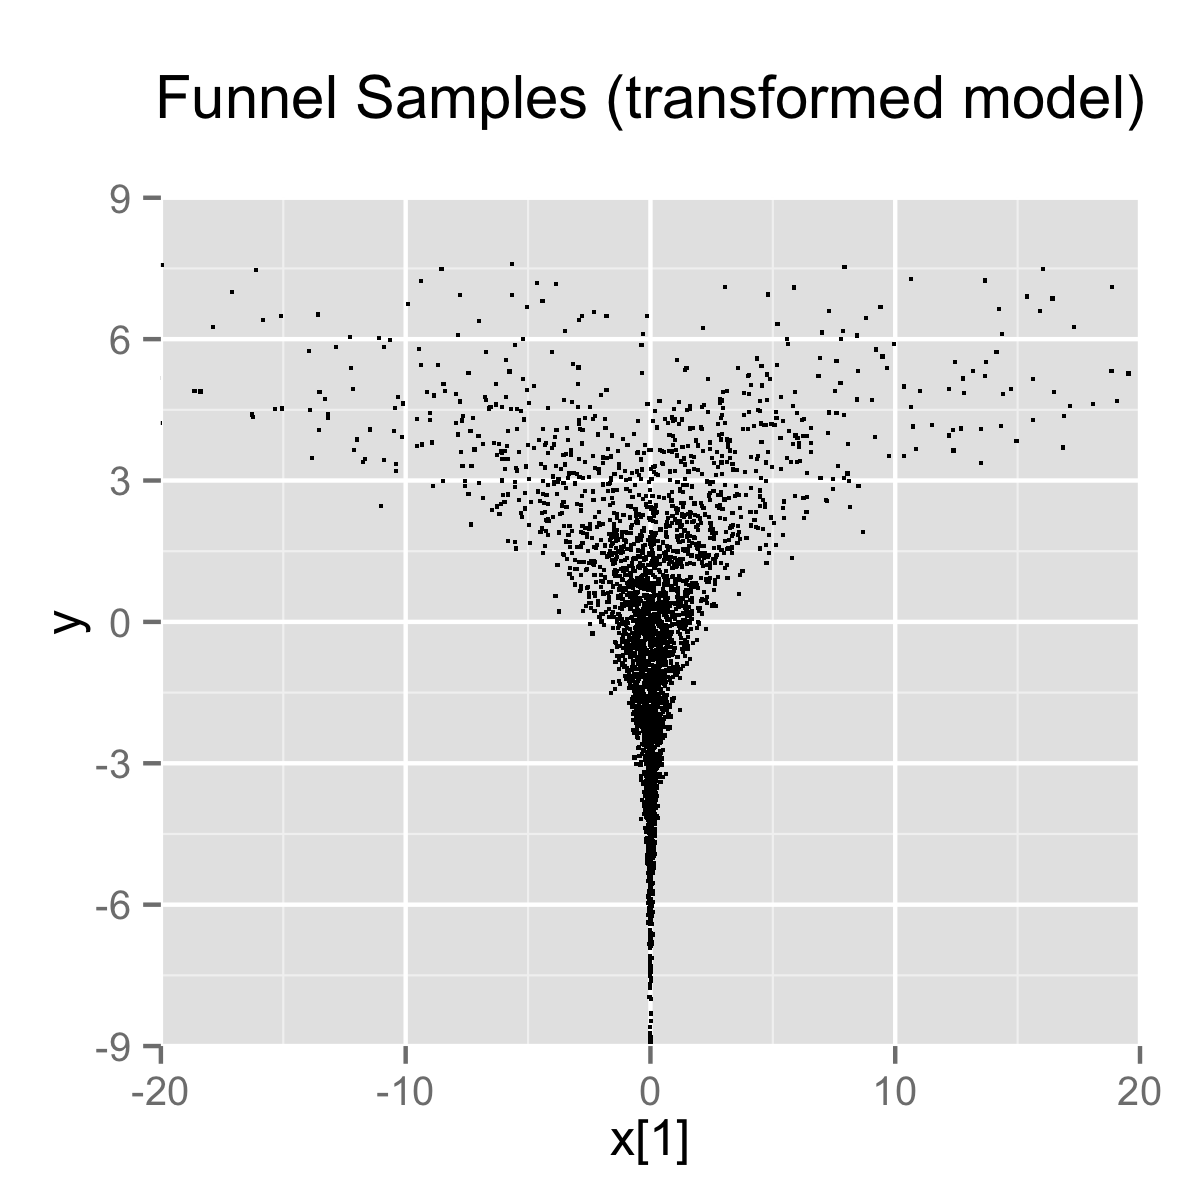
\includegraphics[width=0.4\textwidth]{img/funnel-fit.png}
\end{center}

\sld{Transformed Funnel}
\begin{subitemize}
\item
if $y \sim \distro{Normal}(0,1)$ then
$(\mu + \sigma y) \sim \distro{Normal}(\mu,\sigma)$
\end{subitemize}
\begin{quote}
{\footnotesize
\begin{Verbatim}
parameters {  
  real y_raw;
  vector[9] x_raw;
}
transformed parameters {
  real y;
  vector[9] x;
  y <- 3.0 * y_raw;  
  x <- exp(y/2) * x_raw;
}
model {
  y_raw ~ normal(0,1); // implies y ~ normal(0,3) 
  x_raw ~ normal(0,1); // implies x ~ normal(0,exp(y/2))  
}
\end{Verbatim}
}
\end{quote}


\mypart{Part VI}{Next for Stan}

\sld{Higher-Order Auto-diff}
\begin{itemize}
\item Finish higher-order auto-diff for probability functions
\item May punt some cumulative distribution functions
  \\
  {\footnotesize (Black art iterative algorithms required)}
  \vfill
\item Code complete; under testing
\end{itemize}

\sld{Riemannian Manifold HMC}
\begin{itemize}
\item Best mixing MCMC method (fixed \# of continuous params)
\item Moves on Riemannian manifold rather than Euclidean
\begin{subitemize}
\item adapts to position-dependent curvature
\end{subitemize}
\item \myemph{geoNUTS} generalizes NUTS to RHMC (Betancourt {\slshape arXiv})
\item \myemph{SoftAbs} metric (Betancourt {\slshape arXiv})
\begin{subsubitemize}
\vspace*{-4pt}
\item eigendecompose Hessian and condition
\item computationally feasible alternative to original Fisher info metric
   of Girolami and Calderhead ({\slshape JRSS, Series B})
\item requires third-order derivatives and implicit integrator
\end{subsubitemize}
\vfill
\item Code complete; awaiting higher-order auto-diff
\end{itemize}

\sld{Adiabatic Sampling}
\begin{itemize}
\item Physically motivated alternative to ``simulated''
  \myemph{annealing and tempering} (not really simulated!)
\item Supplies external \myemph{heat bath}
\item Operates through \myemph{contact manifold}
\item System relaxes more naturally between energy levels
\item Betancourt paper on {\slshape arXiv}
  \vfill
\item Prototype complete
\end{itemize}

\sld{Maximum Marginal Likelihood}
\begin{itemize}
\item Fast, Approximate Inference
\item Marginalize out lower-level parameters
\item Optimize higher-level parameters and fix
\item Optimize lower-level parameters given higher-level
\item Errors estimated as in MLE
  \vfill
\item Design complete; awaiting parameter tagging
\end{itemize}

\sld{``Black Box'' EP}
\begin{itemize}
\item Fast, approximate inference (like VB)
\begin{subitemize}
\item VB and EP minimize divergence in opposite directions
\item especially useful for Gaussian processes
\end{subitemize}
%
\item Asynchronous, data-parallel \myemph{expectation propagation}
  (EP)
\item Cavity distributions control subsample variance
%
\vfill
%
\item Prototypte stage
\item {\small collaborating with Seth Flaxman, Aki Vehtari, Pasi
    Jyl\"anki, John Cunningham, Nicholas Chopin, Christian Robert}
\end{itemize}


\mypart{Part VII}{Under Stan's Hood}

\sld{Euclidean Hamiltonian}

\begin{itemize}
\item \myemph{Phase space}: $q$ position (parameters); \ $p$ momentum
\item \myemph{Posterior density}: $\pi(q)$
\item \myemph{Mass matrix}: $M$
\item \myemph{Potential energy}: $V(q) = -\log \pi(q)$
\item \myemph{Kinetic energy}: $T(p) = \frac{1}{2} p^{\top} M^{-1} p$
\item \myemph{Hamiltonian}:  $H(p,q) = V(q) + T(p)$
\item \myemph{Diff eqs}:
  \[
  \frac{dq}{dt} \ = \  + \frac{\partial H}{\partial p}
  \hspace*{48pt}
  \frac{dp}{dt} \ = \ - \frac{\partial H}{\partial q}
  \]
\end{itemize}

\sld{Leapfrog Integrator Steps}
\begin{itemize}
\item Solves Hamilton's equations by \myemph{simulating dynamics}
  \\
  {\footnotesize (symplectic [volume preserving]; $\epsilon^3$ error per step, $\epsilon^2$ total error)}
\item Given: \myemph{step size} $\epsilon$, \myemph{mass matrix} $M$, \myemph{parameters} $q$
\item \myemph{Initialize kinetic} energy, $p \sim {\sf
    Normal}(0,\mbox{\bf I})$
\item \myemph{Repeat} for $L$ leapfrog steps:
  \begin{eqnarray*}
    p & \leftarrow &
    p - \frac{\epsilon}{2} \, \frac{\partial V(q)}{\partial q}
    \ \ \ \ \ \ \mbox{[half step in momentum]}
    \\[6pt]
    q & \leftarrow &
    q + \epsilon \, M^{-1} \, p
    \ \ \ \ \ \ \ \  \mbox{[full step in position]}
    \\[6pt]
    p & \leftarrow &
    p - \frac{\epsilon}{2} \, \frac{\partial V(q)}{\partial q}
    \ \ \ \ \ \ \mbox{[half step in momentum]}
  \end{eqnarray*}
\end{itemize}


\sld{Reverse-Mode Auto Diff}
\begin{itemize}
\item Eval gradient in small multiple of function eval time
  \\
  {\footnotesize (independent of dimensionality)}
\item Templated \myemph{C++ overload} for all functions
\item Code \myemph{partial derivatives} for basic operations
\item Function evaluation builds up \myemph{expression tree}
\item Dynamic program propagates \myemph{chain rule} in reverse pass
\item Extensible w.\ \myemph{object-oriented} custom partial propagation
\item Arena-based \myemph{memory management}
  \\ {\footnotesize (customize \code{operator new})}
\end{itemize}


\sld{Autodiff Expression Graph}
\\
\hspace*{6pt}
\begin{minipage}{0.56\textwidth}
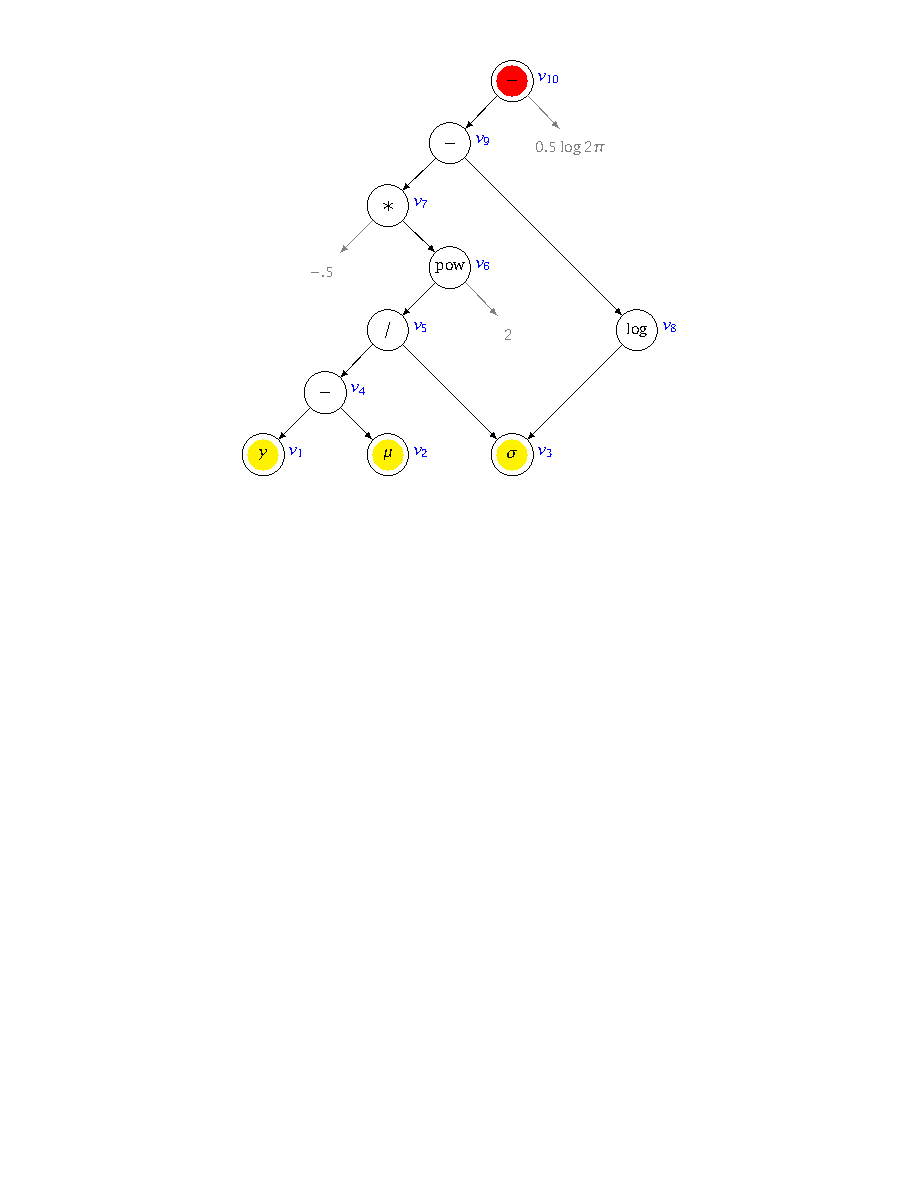
\includegraphics[width=\textwidth]{img/agrad-expression-graph.pdf}
\end{minipage}
\hspace*{-24pt}
\begin{minipage}{0.44\textwidth}
%
\footnotesize
\[
\begin{array}{l}
f(y, \mu, \sigma) 
\\[4pt]
\mbox{ } \ = \ \log \left( \distro{Normal}(y|\mu,\sigma) \right)
\\[4pt]
\mbox{ } \ = \ -\frac{1}{2} \left( \frac{y - \mu}{\sigma} \right)^2
    - \log \sigma
    - \frac{1}{2} \log (2 \pi)
\end{array}
\]
\\
%
\[
\begin{array}{l}
\mbox{ } \hspace*{24pt}
\frac{\partial}{\partial y} f(y,\mu,\sigma)
\\[2pt]
\mbox{ } \hspace*{48pt} = \  -(y - \mu) \sigma^{-2}
\\[8pt]
\mbox{ } \hspace*{24pt} \frac{\partial}{\partial \mu} f(y,\mu,\sigma)
\\[2pt]
\mbox{ } \hspace*{48pt} = \ (y - \mu) \sigma^{-2}
\\[8pt]
\mbox{ } \hspace*{24pt} \frac{\partial}{\partial \sigma} f(y,\mu,\sigma)
\\[2pt]
\mbox{ } \hspace*{48pt} = \ (y - \mu)^2 \sigma^{-3} - \sigma^{-1}
\end{array}
\]
\end{minipage}

\sld{Autodiff Partials}
\begin{center}\footnotesize
\begin{tabular}{c||c|cc}
{\it var} & {\it value} & \multicolumn{2}{|c}{\it partials}
\\ \hline \hline
$v_1$ & $y$ 
\\[2pt]
$v_2$ & $\mu$
\\[2pt]
$v_3$ & $\sigma$
\\[2pt]
$v_4$ & $v_1 - v_2$ & $\partial v_4 / \partial v_1 = 1$ 
                   & $\partial v_4 / \partial v_2 = -1$
\\[4pt]
$v_5$ & $v_4 / v_3$ & $\partial v_5 / \partial v_4 = 1/v_3$
                    & $\partial v_5 / \partial v_3 = -v_4 v_3^{-2}$
\\[4pt]
$v_6$ & $\left(v_5\right)^2$
      & \multicolumn{2}{c}{$\partial v_6 / \partial v_5 = 2 v_5$}
\\[4pt]
$v_7$ & $(-0.5) v_6$ & \multicolumn{2}{c}{$\partial v_7 / \partial v_6
                                          = -0.5$}
\\[4pt]
$v_8$ & $\log v_3$ & \multicolumn{2}{c}{$\partial v_8 / \partial v_3 = 1/v_3$}
\\[4pt]
$v_9$ & $v_7 - v_8$ & $\partial v_9 / \partial v_7 = 1$
                    & $\partial v_9 / \partial v_8 = -1$
\\[4pt]
$v_{10}$ & $v_9 - (0.5 \log 2\pi)$ 
         & \multicolumn{2}{c}{$\partial v_{10} / \partial v_9 = 1$}
\end{tabular}
\end{center}

\sld{Autodiff: Reverse Pass}
{\small
\[
\begin{array}{rcl|l}
{\it var} & {\it operation} & {\it adjoint} & {\it result}
\\ \hline \hline
a_{1:9} & = & 0 & a_{1:9} = 0
\\
a_{10} & = & 1 & a_{10} = 1
\\ \hline
a_{9} & {+}{=} & a_{10} \times (1) & a_9 = 1
\\
a_{7} & {+}{=} & a_9 \times (1) & a_7 = 1
\\
a_{8} & {+}{=} & a_9 \times (-1) & a_8 = -1
\\
a_{3} & {+}{=} & a_8 \times (1 / v_3) & a_3 = -1 / v_3
\\
a_{6} & {+}{=} & a_7 \times (-0.5) & a_6 = -0.5
\\
a_{5} & {+}{=} & a_6 \times (2 v_5) & a_5 = -v_5
\\
a_{4} & {+}{=} & a_5 \times (1 / v_3) & a_4 = -v_5 / v_3
\\
a_{3} & {+}{=} & a_5 \times (-v_4 v_3^{-2}) & a_3 = -1 / v_3 + v_5 v_4 v_3^{-2}
\\
a_{1} & {+}{=} & a_4 \times (1) & a_1 = -v_5 / v_3
\\
a_{2} & {+}{=} & a_4 \times (-1) & a_2 = v_5 / v_3
\end{array}
\]
}

\sld{Forward-Mode Auto Diff}
\begin{itemize}
\item Templated \myemph{C++ overload} for all functions
\item Code \myemph{partial derivatives} for basic operations
\item Function evaluation propagates \myemph{chain rule} forward
\item Nest reverse-mode in forward for \myemph{higher-order}
\item \myemph{Jacobians}
  \vspace*{-4pt}
  \begin{itemize}\small
  \item Rerun propagation pass in reverse mode
  \item Rerun forward construction with forward mode
  \end{itemize}
  \vfill
\item Faster autodiff rewrite coming in six months to one year
\end{itemize}

\sld{Autodiff Functionals}

\begin{itemize}
\item Fully encapsulates autodiff in C++
\item Autodiff operations are functionals {\footnotesize (higher-order functions)}
  \begin{itemize}\small
  \item gradients, Jacobians, gradient-vector product
  \item directional derivative
  \item Hessian-vector product
  \item Hessian
  \item gradient of trace of matrix-Hessian product
    \\ {\footnotesize (for SoftAbs RHMC)}
  \end{itemize}
\item Functions to differentiate coded as functors (or pointers)
  \\ {\footnotesize (enables dynamic C++ bind or lambda)}
\end{itemize}

\sld{Variable Transforms}
\begin{itemize}
\item Code HMC and optimization with $\mathbb{R}^n$ \myemph{support}
\item Transform constrained parameters to unconstrained
  \vspace*{-2pt}
  {\small
    \begin{itemize}
    \item lower (upper) bound: offset (negated) log transform
    \item lower and upper bound: scaled, offset logit transform
    \item simplex: centered, stick-breaking logit transform
    \item ordered: free first element, log transform offsets
    \item unit length: spherical coordinates
    \item covariance matrix: Cholesky factor positive diagonal 
    \item correlation matrix: rows unit length via quadratic stick-breaking
    \end{itemize}
  }
\end{itemize}


\sld{Variable Transforms (cont.)}
\begin{itemize}
\item Inverse transform from unconstrained $\mathbb{R}^n$
\item Evaluate log probability in model block on natural scale
\item Optionally adjust log probability for change of variables
  \\ {\footnotesize (add log determinant of inverse transform Jacobian)}
\end{itemize}

\sld{Parsing and Compilation}
\begin{itemize}
\item Stan code \myemph{parsed} to abstract syntax tree (AST)
  \\ {\footnotesize (Boost Spirit Qi, recursive descent, lazy semantic
    actions)}
\item C++ model class \myemph{code generation} from AST
  \\ {\footnotesize (Boost Variant)}
\item C++ code \myemph{compilation}
\item \myemph{Dynamic linking} for RStan, PyStan
\end{itemize}

\sld{Coding Probability Functions}
\begin{itemize}
\item \myemph{Vectorized} to allow scalar or container arguments
  \\ {\footnotesize (containers all same shape; scalars broadcast as necessary)}
\item Avoid \myemph{repeated computations}, e.g. $\log \sigma$ in
  \hspace*{-18pt}
  {\small
    \begin{eqnarray*}
      \textstyle \log \, \mbox{\sf Normal}(y | \mu, \sigma)
      & = & \textstyle \sum_{n=1}^N \log \, \mbox{\sf Normal}(y_n | \mu,\sigma)
      \\[4pt]
      & = & \textstyle \sum_{n=1}^N  - \log \sqrt{2\pi} \ - \log \sigma \ -
      \frac{\textstyle y_n - \mu}{\textstyle 2\sigma^2}
    \end{eqnarray*}
  }
\item recursive \myemph{expression templates} to broadcast and cache scalars,
  generalize containers (arrays, matrices, vectors)
\item \myemph{traits} metaprogram to \myemph{drop constants} (e.g., $-\log
  \sqrt{2 \pi}$ or $\log \sigma$ if constant) 
  and calculate intermediate and return types
\end{itemize}


\mypart{}{The End}

\sld{Stan's Namesake}
\begin{itemize}
\item Stanislaw Ulam (1909--1984)
\item Co-inventor of Monte Carlo method (and hydrogen bomb)
\item[]
  \begin{center}
    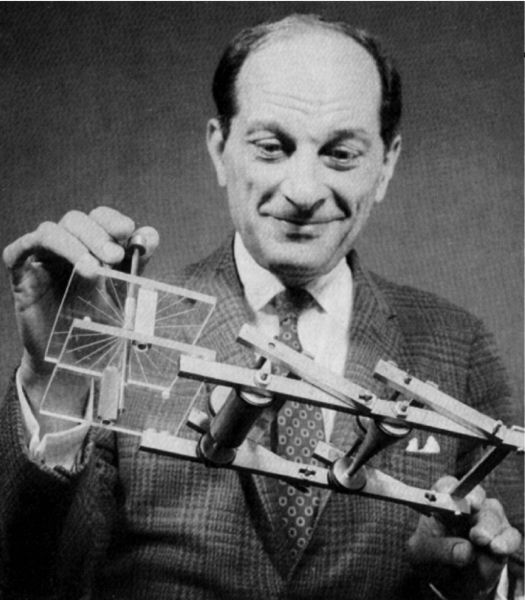
\includegraphics[width=0.25\textwidth]{img/ulam-fermiac.jpg}
  \end{center}
  {\small
  \item Ulam holding the Fermiac, Enrico Fermi's physical Monte Carlo simulator
    for random neutron diffusion}
\end{itemize}



\end{document}